\documentclass[a4paper, fontsize = 8pt, landscape]{scrartcl}
\usepackage{../../../misc_files/LateX/layout_and_colours}
\makeatletter
\def\input@path{{content/lecture_summary/}{content/examples/}{content/recap/analysis/}{content/recap/linalg/}{content/recap/hm1/}}
\makeatother
\graphicspath{{content/images/}{content/lecture_summary/images/}{content/examples/images/}{content/recap/analysis/images/}{content/recap/linalg/images/}{content/recap/hm1/images/}}

\title{HM2 recap}
\author{Jil Zerndt}
\date{FS 2025}

\createtitlepagestyle
\createmainpagestyle
\begin{document}
\begin{multicols}{3}
	\thispagestyle{TitlePageStyle}
	\maketitle
	\sffamily
	%Basics
	
\begin{lemma}{Mitternachtsformel}
    $x=\frac{-b\pm\sqrt{b^2-4ac}}{2a}$
\end{lemma}

\begin{formula}{Polynomdivision} \emph{!} Vorzeichen von Nullstellen umdrehen\\
    $\frac{P(x)}{q(x)} = S(x) + \frac{r(x)}{q(x)}$ \qquad $P,q,S,r$ Polynome
$$
\begin{array}{cc}
\left(x^3-2 x^2-5 x-6\right):(x-1)=x^2-x-6 & \mid x^3: x=x^2 \\
-\left(x^3-x^2\right) & \mid-x^2: x=-x \\
-x^2-5 x & \\
-\left(x^2-x\right) & \mid-6 x: x=-6 \\
\hline-(-6 x+6) &
\end{array}
$$

Eine Polynomfunktion vom Grad $n$ hat höchstens $n$ reelle Nullstellen.
$$
f(x)=a_n \cdot\left(x-x_1\right) \cdot\left(x-x_2\right) \cdot \ldots \cdot\left(x-x_n\right)
$$
\end{formula}

\begin{definition}{Kardinalität}
    \begin{itemize}
        \item X, Y \emph{gleichmächtig}, falls es eine \underline{Bijektion} $f: X \to Y$ gibt.
        \item X \emph{endlich}, falls entweder $X = \emptyset$ ($\card X = 0$) oder $\exists n \in \N$, sodass $X$ und $\{1,2,\ldots,n\}$ ($\card X = n$) gleichmächtig sind.
        \item X \emph{abzählbar}, falls sie endlich oder gleichmächtig wie $\N$ ist.
    \end{itemize}
\end{definition}
\begin{definition}{Beschränktheit}
    $A \subseteq \R$ eine Teilmenge.
    \begin{itemize}
        \item $c \in \R$ ist eine \emph{obere Schranke} von A falls $\forall a \in A: a\leq c$ ($A$ \textit{nach oben beschränkt}).
        \item $c \in \R$ ist eine \emph{untere Schranke} von A falls $\forall a \in A: a \geq c$ ($A$ \textit{nach unten beschränkt}).
        \item $A$ heisst \textit{beschränkt}, wenn nach oben und unten beschränkt.
        \item \emph{Maximum} von $A$ falls $m \in A$ und $m$ obere Schranke.
        \item \emph{Minimum} von $A$ falls $m \in A$ und $m$ untere Schranke.
    \end{itemize}
\end{definition}


\begin{definition}{Intervalle}
    Ein \emph{abgeschlossenes Intervall} ist eine Teilmenge $I \subseteq \R$ der Form
    \begin{itemize}
        \item Abgeschlossen:
            $[a, b]=\{x \in \mathbb{R} \mid a \leq x \leq b\}$
        \item Offen:
            $(a, b)=\{x \in \mathbb{R} \mid a<x<b\}$
        \item Halboffen:
            $[a, b)=\{x \in \mathbb{R} \mid a \leq x<b\}$
        \item Unendlich:
            $[a, \infty)=\{x \in \mathbb{R} \mid a \leq x\}$
    \end{itemize}
\end{definition}

\begin{definition}{Supremum und Infimum}
    $A \subseteq \R, ~A\neq \emptyset$
    \begin{enumerateroman}
        \item $A$ nach oben beschränkt. Dann gibt es eine kleinste obere Schranke von $A$: $c \coloneqq \sup A$. Das \emph{Supremum} von $A$.
        \item $A$ nach unten beschränkt. Dann gibt es eine kleinste untere Schranke von $A$: $c \coloneqq \inf A$. Das \emph{Infimum} von $A$.
    \end{enumerateroman}
    \tcblower 
    Vereinfacht formuliert: Für ein abgeschlossenes, halboffenes oder offenes Intervall $[a,b], [a,b), (a,b]$ oder $(a,b)$ gilt $inf = a$, $sup = b$ (solange $a, b \neq \infty$)
\end{definition}

\begin{definition}{Monotonie}
    \begin{enumerate}
        \item $\sequence$ \emph{monoton wachsend} falls: \null\hfill $a_n \leq a_{n + 1} \quad \forall n \geq 1$.
    	\item $\sequence$ \emph{monoton fallend} falls: \null\hfill $a_n \geq a_{n+1} \quad \forall n \geq 1$.
    \end{enumerate}
\end{definition}

\begin{KR}{Monotonie zeigen}
    \begin{itemize}
  \item $a_{n+1}-a_{n} \geq 0 \Rightarrow$ monoton wachsend (bzw. umgekehrt fallend)
  \item $\frac{a_{n+1}}{a_{n}} \geq 1$ und $a_{n} \geq 0$ dann monoton wachsend
\end{itemize}
\end{KR}

\raggedcolumns
\columnbreak

\subsubsection{Trigonometrische Funktionen}

\begin{iequation}[align*]
	\tikz[remember picture] \coordinate(sinanchor) at (0,0); \sin x &= \sum_{n=0}^{\infty} \frac{(-1)^n x^{2n + 1}}{(2n+1)!} = x - \frac{x^3}{3!} + \frac{x^5}{5!}\ldots ~ \text{stetig}\\
	\tikz[remember picture] \coordinate(cosanchor) at (0,0); \cos x &= \sum_{n=0}^{\infty} \frac{(-1)^n x^{2n}}{(2n)!} = 1 - \frac{x^2}{2!} + \frac{x^4}{4!}\ldots \hspace{3.8mm} \text{stetig}\\
	\tan x &= \frac{\sin x}{\cos x} \hspace{10mm} \cot x = \frac{\cos x}{\sin x} \tikz[remember picture] \coordinate(trigfunkanchor) at (0,0);
\end{iequation}
\begin{tikzpicture}[remember picture, overlay]
	\node[overlaynote, text width = 28mm, anchor = west] at ($(trigfunkanchor) + (0.5,0.25)$) {$\pi$: kleinste strikt positive Nullstelle von $\sin$.};
	\node[overlaynote, rotate = 90] at ($(trigfunkanchor) + (3,2)$) {$\cos(x) = \sin \left(x + \frac{\pi}{2}\right)$};
	\node[overlaynote, rotate = 20, above left = 3mm and 2mm of sinanchor] (sinnote) {ungerade};
	\draw[overlayarrow] (sinnote) to[bend right] (sinanchor);
	\node[overlaynote, rotate = 20, above left = 3mm and 2mm of cosanchor] (cosnote) {gerade};
	\draw[overlayarrow] (cosnote) to[bend right] (cosanchor);
\end{tikzpicture}

\begin{center}
    \renewcommand{\arraystretch}{1.3} %Zeilenabstand verändern
    \setlength{\tabcolsep}{4pt}
    \begin{tabular}{|c|c|c|c|c|c|c|c|c|c|}
        \hline
        Grad            & $0^\circ$ & $30^\circ$           & $45^\circ$           & $60^\circ$           & $90^\circ$      & $120^\circ$          & $135^\circ$           & $150^\circ$           & $180^\circ$ \\
        \hline
        $\varphi$       & $0$       & $\frac{\pi}{6}$      & $\frac{\pi}{4}$      & $\frac{\pi}{3}$      & $\frac{\pi}{2}$ & $\frac{2\pi}{3}$     & $\frac{3\pi}{4}$      & $\frac{5\pi}{6}$      & $\pi$       \\
        \hline
        $\sin(\varphi)$ & $0$       & $\frac{1}{2}$        & $\frac{\sqrt{2}}{2}$ & $\frac{\sqrt{3}}{2}$ & $1$             & $\frac{\sqrt{3}}{2}$ & $\frac{\sqrt{2}}{2}$  & $\frac{1}{2}$         & $0$         \\
        \hline
        $\cos(\varphi)$ & $1$       & $\frac{\sqrt{3}}{2}$ & $\frac{\sqrt{2}}{2}$ & $\frac{1}{2}$        & $0$             & $-\frac{1}{2}$       & $-\frac{\sqrt{2}}{2}$ & $-\frac{\sqrt{3}}{2}$ & $-1$        \\
        \hline
        $\tan(\varphi)$ & $0$       & $\frac{\sqrt{3}}{3}$ & $1$                  & $\sqrt{3}$           & $\pm \infty$    & -$\sqrt{3}$          & $-1$                  & $-\frac{\sqrt{3}}{3}$ & $0$         \\
        \hline
    \end{tabular}
\end{center}





\begin{theorem}{Eigenschaften sin/cos}
    \begin{enumerate}
        \item $\exp ix = \cos(x) + i \sin(x) \quad \forall x \in \mathbb{C}$
        \item $\cos x = \cos(-x) ~\text{und}~ \sin(-x) = -\sin x \quad\forall x \in \mathbb{C}$
        \item $\sin(x + y) = \sin(x)\cos(y) + \cos(x)\sin(y)$
        \item $\cos(x + y) = \cos(x)\cos(y) - \sin(x)\sin(y)$
        \item $\cos^2(x) + \sin^2(x) = 1 \quad \forall x \in \mathbb{C}$ 
        \item $\sin x = \frac{e^{iz} - e^{-iz}}{2i}, \quad \cos x = \frac{e^{iz} + e^{-iz}}{2}$
    \end{enumerate} 
 \end{theorem}
 
 \begin{corollary}{Winkelverdopplung}\\
         $\sin(2x) = 2 \sin(x)\cos(x)$ \hspace{4mm} $\cos(2x) = \cos^2(x) - \sin^2(x)$
 \end{corollary}
 \begin{corollary}{Potenz der Winkelfunktion}\\
    $$\sin^2(x) = \frac{1 - \cos(2x)}{2} \quad \cos^2(x) = \frac{1 + \cos(2x)}{2}$$
     %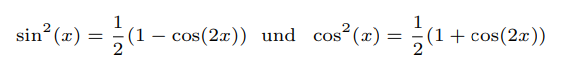
\includegraphics[scale=0.5]{Analysis1/zsf/Images/Basics/potenz_winkelfunktion.png}
 \end{corollary}
 \begin{corollary}{Eigenschaften mit $\pi$}
     \begin{enumerate}[itemsep= 2pt]
         \item $e^{i\pi} = -1, \quad e^{2i\pi} = 1$
         \item $\sin\left(x + \frac{\pi}{2}\right) = \cos(x), \quad \cos\left(x + \frac{\pi}{2}\right) = -\sin(x)$
         \item $\sin(x+\pi) = -\sin (x), \quad \sin(x + 2\pi) = \sin(x)$
         \item $\cos(x+\pi) = -\cos (x), \quad \cos(x + 2\pi) = \cos(x)$
     \end{enumerate}
 \end{corollary}

 \begin{corollary}{Nullstellen von trigonometrischen Funktionen}
    \begin{enumerate}
         \item $\text{Nullstellen Sinus} = \{k\cdot \pi : k\in \mathbb{Z}\}$\\
        $\sin(x) > 0 \quad \forall x \in ]2k\pi, ~(2k+1)\pi[, ~ k\in \mathbb{Z}$\\[2pt]
        $\sin(x) < 0 \quad \forall x \in ](2k + 1)\pi, ~(2k+2)\pi[, ~ k\in \mathbb{Z}$
        \item $\text{Nullstellen Cosinus} = \left\{\frac{\pi}{2}+k\cdot \pi : k\in \mathbb{Z}\right\}$\\
        $\cos(x) > 0:\forall x \in \left]-\frac{\pi}{2} +2k\pi, ~-\frac{\pi}{2} +(2k+1)\pi\right[, ~ k\in \mathbb{Z}$\\[2pt]
        $\cos(x) < 0:\forall x \in \left]-\frac{\pi}{2} + (2k + 1)\pi, ~-\frac{\pi}{2} +(2k+2)\pi\right[, ~ k\in \mathbb{Z}$
    \end{enumerate}
\end{corollary}
\noindent Für $\tan(x)$ gilt $x \notin \frac{\pi}{2} + \pi \cdot \Z$ \qquad Für $\cot(x)$ gilt $x \notin \pi \Z$
 

\raggedcolumns
\columnbreak

\subsubsection{Relle Exponentialfunktion}
\begin{center}
    \hfill
    \begin{minipage}{0.3\linewidth}
        \begin{iequation}
            \exp (z) \coloneqq \sum_{n=0}^\infty \frac{z^n}{n!}
        \end{iequation}
    \end{minipage}
    \hfill
    \begin{minipage}{0.6\linewidth}
        \begin{theorem}{Eigenschaften}
            $\exp : \R \to ]0, + \infty[$ ist streng monoton wachsend, stetig und surjektiv.
        \end{theorem}       
    \end{minipage}
    \hfill
\end{center}

%\begin{center}
    \begin{minipage}{0.5\linewidth}
        \begin{iequation}[align*]
            \exp(-x)\exp(x) &= 1\\
	    \text{\textbf{\textsf{}}} \quad\exp(x) &> 0 \qquad\forall x \in \R \tikz[remember picture, overlay]
	    \coordinate(expineq) at (0,0);\\
            \exp(x) &> 1 \qquad\forall x > 0\\
            \exp(a+b) &= \exp(a) \cdot \exp(b)\\ 
            \exp(a-b) &= \exp(a) \div \exp(b)
        \end{iequation}
\begin{tikzpicture}[overlay, remember picture]
	\node[overlaynote, above right = 8mm and 0mm of expineq] (expineqnote) {Aber nicht: $\exp(z) > 0 \quad \forall z \in \C$};
\end{tikzpicture}
    \end{minipage}
    \hfill
    \begin{minipage}{0.48\linewidth}
        \begin{corollary}
            \\$\exp(z) > \exp(y) \quad \forall z > y$
        \end{corollary}
        \begin{corollary}
            \\${\exp (x) \geq 1 + x \quad \forall x \in \R}$
        \end{corollary}    
        \begin{corollary}
            \\$e^{\alpha x} = \sum_{n=0}^\infty \frac{\alpha^n x^n}{n!}$
        \end{corollary}
    \end{minipage}
%\end{center}
$\exp(z) = \exp(y + (z-y)) = \exp(y) \exp(z-y)\\
            \exp(x) = \lim_{n\to \infty}(1 + \frac{x}{n})^n$\\
 \begin{minipage}{0.6\linewidth}
        \begin{align*}
            \exp(\ln a + \ln b) &= \exp(\ln a) \cdot \exp (\ln b)\\
            \exp(\ln a)\exp(\ln b) &= ab = \exp(\ln ab)\\
            \exp(\ln a + \ln b) &= \exp(\ln ab)\\
            \ln a + \ln b &= \ln (ab)
        \end{align*}
    \end{minipage}
    \hfill
    \begin{minipage}{0.35\linewidth}
        \begin{iequation}
            x^a \coloneqq \exp(a \ln x)
        \end{iequation}
    \end{minipage}

    \subsubsection*{Logarithmen}
\begin{corollary}{Rechnen mit Logarithmen}
    \begin{enumerate}
        \item Für $a > 0$ ist $]0, \infty[ \to ]0 + \infty[$ \quad $x \mapsto x^a$ eine stetige, streng monoton wachsende Bijektion.
        \item Für $a < 0$ ist $]0, \infty[ \to ]0 + \infty[$ \quad $x \mapsto x^a$ eine stetige, streng monoton fallende Bijektion.
        \item $\ln (a \cdot b) = \ln a + \ln b \quad \forall a,b \in ]0 +  \infty[$
        \item $\ln (a \div b) = \ln a - \ln b \quad \forall a,b \in ]0 +  \infty[$
        \item ${\ln \left(x^a\right) = a \ln (x) \quad \forall a \in \R, \forall x > 0}$
        \item ${x^a \cdot x^b = x^{a+b} \quad a,b \in \R, \forall x > 0}$
        \item ${\left(x^a\right)^b = x^{a \cdot b} \quad \forall a,b \in \R, \forall x > 0}$
    \end{enumerate}
    Im Allgemeinen gilt: $log_b (a) = \frac{ln(a)}{ln(b)}$
\end{corollary}

\begin{formula}{ln(1 + x)}
       $ = \sum_{n=1}^\infty \frac{(-1)^{n-1}x^n}{n} \quad \text{für} \quad |x| < 1$
\end{formula}

\subsubsection{Werte von log}
\begin{equation*}
	\begin{array}{lccccccc}
		& 0 & 1 & 2 & e & 3 & 5 & 10\\
		\ln & - \infty & 0 & 0.693 & 1 & 1.09 & 1.609 & 2.303\\
		\log_2 & - \infty & 0 & 1 & 1.443 & 1.585 & 2.321 & 3.321\\
		\log_{10} & - \infty & 0 & 0.301 & 0.434 & 0.477 & 0.699 & 1
	\end{array}
\end{equation*}

\begin{center}
    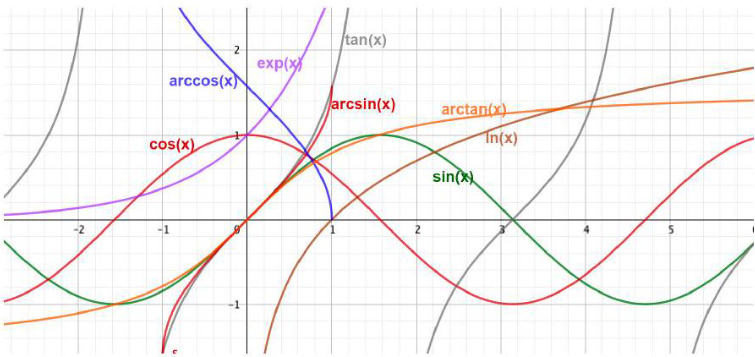
\includegraphics[width=0.8\linewidth]{trigonometrische_funktionen.png}
\end{center}










	\raggedcolumns
	\pagebreak
	%Analysis
	

\begin{definition}{$\varepsilon$-Definition}
    \\Folge $\sequence$ heisst \emph{konvergent}, falls es $l \in \R$ gibt, sodass \vspace{1mm}
    
    $\forall \varepsilon > 0$ die Menge $\{n \in \N^* : a_n \notin~] l - \varepsilon, l + \varepsilon[\,\}$ endlich ist. ($\N^*$: $\N$/$0$.) \vspace{1mm} \\ 
    Einfach gesagt: das heisst, dass $|a_n - a| < \epsilon$ ab einem gewissen n für alle $\epsilon$ gilt.
   
\end{definition}
Bem: $l$ bezeichnet den Grenzwert $\lim_{n \to \infty} a_n$
\begin{definition}{Formelle Grenzwert Definition}
    Folgende Aussagen sind äquivalent:
    \begin{enumerate}
        \item $\sequence$ konvergiert gegen $l = \lim_{n \to \infty} a_n$
        \item $\forall \varepsilon > 0~\exists N \geq 1$, sodass $|a_n -l | < \varepsilon \quad \forall n \geq N$.
    \end{enumerate}
\end{definition}
\begin{lemma}{Einzigartigkeit Grenzwert}
     Es gibt max. ein $l \in \R$ für $a_n$ mit dieser Eigenschaft (max. 1 Grenzwert)
\end{lemma}
\begin{theorem}{Rechenregeln mit Folgen}
    \\Sei $\sequence,\sequence[b]$ konvergente Folgen mit$a = \lim_{n \to \infty} a_n$, $b = \lim_{n \to \infty} b_n$
    \begin{enumerate}
        \item $(a_n \pm b_n)_{n \geq 1}$ konvergent, $\lim_{n \to \infty} (a_n \pm b_n) = a \pm b$.
        \item $(a_n \cdot b_n)_{n \geq 1}$ konvergent, $\lim_{n \to \infty} (a_n \cdot b_n) = a \cdot b$.
        \item $(a_n \div  b_n)_{n \geq 1}$ konvergent, $\lim_{n \to \infty} (a_n \div b_n) = a \div b$.
        \\(solange $b_n \neq 0 ~ \forall n \geq 1$ und $b \neq 0$)
        \item Falls $\exists K \geq 1$ mit $a_n \leq b_n ~ \forall n \geq K$ folgt $a \leq b$.
    \end{enumerate}
\end{theorem}






	\raggedcolumns
	\pagebreak
	\section{Integralrechnung}

\subsection{Integrationsregeln}

\begin{definition}{Integrale von Linearkombinationen}
	Gegeben:
	\[\int{f(x)\mathrm{d}x} = F(x)+C, \quad  \int{g(x)\mathrm{d}x} = G(x)+C\]
	Das unbestimmte Integral der Linearkombination \(\lambda_1f(x) + \lambda_2g(x)\) ist:
	\[\int{(\lambda_1f(x)+\lambda_2g(x))} = \lambda_2F(x)+\lambda_2G(x)+C \quad (\lambda_1,\lambda_2 \in \mathbb{R} )\]
\end{definition}
\begin{definition}{Integral von verschobenen Funktionen}
	Gegeben:
	\[\int{f(x)\mathrm{d}x} = F(x) + C \]
	Das unbestimte integral um Betrag k in x-Richtung verschoben ist:
	\[\int{f(x-k)\mathrm{d}x}= F(x-k)+C \quad (k \in \mathbb{R}) \]
\end{definition}
\begin{definition}{Integrale von gestreckten Funktionen}
	Gegeben:
	\[\int{f(x)\mathrm{d}x} = F(x)+C \]
	Das unbestimmte Integral um Faktor k in x-Richtung gestreckt ist:
	\[\int{f(k\cdot x)\mathrm{d}x}= \frac{1}{k}F(k\cdot x)+C \quad (k\neq0 )\]
\end{definition}

\begin{concept}{Integralregeln}
    \begin{itemize}
      \item Addition/Subtraktion:
      $\int f(x-k) d x=F(x-k)+C$
      \item Multiplikation:
      $\int f(x \cdot k) d x=\frac{1}{k} F(x \cdot k)+C$
      \item Skalarmultiplikation:
      $\int \lambda_{1} f(x)+\lambda_{2} g(x) d x=\lambda_{1} F(x)+\lambda_{2} G(x)+C$
    \end{itemize}
\end{concept}


\begin{KR}{Strategie zur Berechnung von Integralen}
    \\\emph{Bruchform:}
    \begin{enumerate}
        \item Vereinfache, so dass ein einfacher Nenner entsteht
        \item Partialbruchzerlegung
        \item $\frac{u'}{2\sqrt{u}}$ oder $\frac{u'}{u}$ erkennen $\Rightarrow \sqrt{u}$ oder $log|u|$
    \end{enumerate}
    \emph{Produktform:}
    \begin{enumerate}
        \item Partielle Integration anwenden (evtl. mehrmals)
        \item Kettenregel verwenden
    \end{enumerate}
    \emph{Potenzen:}\\
        $\int_{a}^{b} f(x)^{c} d x$ umformen in $\int_{a}^{b}(f(x)^{c} \cdot 1) d x$ oder $\int_{a}^{b}(f(x)^{c-1} \cdot f(x)) d x$ um dann partielle Integration anzuwenden\\
    \emph{Exponentenform:}\\
        $e / \log$ Trick verwenden, wenn Variabel im Exponenten ist.\\
    \emph{Produkt mit $e, \sin , \cos$}\\
        Mehrmals partielle Integration anwenden, wobei sin, cos immer $g^{\prime}$ und immer $f$ ist.\\
    \emph{Summe im Integral:}\\
        Summe aus dem Integral herausziehen (dafür muss die Reihe gleichmässig konvergieren)
\end{KR}

Symmetrie ungerader Funktionen beachten: (alls Funktion ungerade ist und symmetrische Grenzen hat)
$\int_{-\frac{\pi}{2}}^{\frac{\pi}{2}} \underbrace{(\sin x)^7 \cos x}_{\text{ungerade}} \dif x = 0$


\subsubsection{Integrationsmethoden}
\paragraph{Partielle Integration}

\begin{concept}{Partielle Integration}
	Seien $a < b$ reelle Zahlen und $f,g:[a,b] \to \R$ stetig differenzierbar. Dann gilt:
   \begin{equation*}
	   \int_a^b f(x) g'(x) \dif x = f(b) g(b) - f(a) g(a) - \int_a^b f'(x)g(x) \dif x
   \end{equation*}
   bzw. für unbestimmte Integrale\\

   $
   \int\left(f(x) \cdot g^{\prime}(x)\right) d x=f(x) \cdot g(x)-\int\left(f^{\prime}(x) \cdot g(x)\right) d x
   $
\end{concept}
\begin{remark}
   $\uparrow 1$ falls arc- oder log-Funktion vorkommt, $x^{n}, \frac{1}{1-x^{2}}, \frac{1}{1+x^{2}}$\\

   $\downarrow x^{n}, \arcsin (x), \arccos (x), \arctan (x)$,
\end{remark}
\begin{KR}{Prioritäten}$f(x)$ nach folgender Priorität auswählen:\\
   $
   \begin{array}{lllll}
	   1. \log_e, \log_a  & 2. \arcsin, \arccos &  3. x^2, 5x^3 & 4. \sin, \cos, \tan & 5. e^x, 5a^x
   \end{array}
   $
\end{KR}

\paragraph*{Substitution}

\begin{concept}{Substitution}\\
    Die Substitution ist die Umkehrung der Kettenregel. D.h. wir wollen Substitution vorallem verwenden, wenn wir innere Funktionen haben.
    \begin{equation*}
        \int_{g(b)}^{g(a)} f(x) \dif x = \int_{a}^b f(g(t)) g'(t) \dif t
    \end{equation*}
    bzw. für unbestimmte Integrale

    $$
    \int f(g(t)) \cdot g^{\prime}(t) d t=\left.\int f(x) d x\right|_{x=g(t)}
    $$
\end{concept}




\begin{corollary}{Nützliche Regeln}
	Sei $I \subseteq \R$ ein Intervall und $f: I \to \R$ stetig.
	\begin{enumerate}
		\item Seien $a,b,c \in \R$, sodass das abgeschlossene Intervall mit den Endpunkten $a+c$, $b+c$ in $I$ enthalten ist.
			Dann gilt
			\begin{equation*}
				\int_{a+c}^{b+c} f(x) \dif x = \int_{a}^{b} f(t+c) \dif t
			\end{equation*}
		\item Seien $a,b,c \in \R$ mit $c \neq 0$, sodass das abgeschlossene Intervall mit Endpunkten $ac$, $bc$ in $I$ enthalten ist.
			Dann gilt
			\begin{equation*}
				\int_{a}^{b} f(ct) \dif t = \frac{1}{c} \int_{ac}^{bc} f(x) \dif x
			\end{equation*}
	\end{enumerate}
\end{corollary}

\begin{KR}{Nützliche Substitutionen}
    \begin{itemize}
        \item $\log (x)$ subst: $t=\log (x), x=e^{t}, d x=e^{t} d t$
        \item für gerade $n: \cos ^{n}(x), \sin ^{n}(x), \tan (x)$ \\Sub: $t=\tan (x)$, $d y=\frac{1}{1+t^{2}} d t, \sin ^{2}(x)=\frac{t^{2}}{1+t^{2}}, \cos ^{2}(x)=\frac{1}{1+t^{2}}$
        \item für ungerade $n: \cos ^{n}(x), \sin ^{n}(x)$, \\Sub: $t=\tan (x / 2)$, $d y=\frac{2}{1+t^{2}} d t, \sin (x)=\frac{2 t}{1+t^{2}}, \cos (x)=\frac{1-t^{2}}{1+t^{2}}$
        \item $\int \sqrt{1-x^{2}} d x$ sub: $x=\sin (x)$ oder $\cos (x)$
        \item $\int \sqrt{1+x^{2}} d x$ sub: $x=\sinh (x)$
    \end{itemize}
\end{KR}




\begin{formula}{Substitution unbestimmtes Integral}
    \begin{itemize}
	\item Aufstellen und Ableiten der Substitutionsgleichungen:\\
	    $u=g(x),\quad \frac{\mathrm{d}u}{\mathrm{d}x}=g'(x),\quad \mathrm{d}x = \frac{\mathrm{d}u}{g'(x)} $
	\item Durchführen der Substitution \(u=g(x) \)	 und \(\mathrm{d}x=\frac{\mathrm{d}u}{g'(x)} \) in \\das  
	    integral $\int{f(x)\mathrm{d}x}$:
	    \[\int{f(x)\mathrm{d}x}=\int{r(u)}{\mathrm{d}u} \]
	\item Berechnen des Integrals mit Variable u:
	    $$\int{r(u)\mathrm{d}u}=R(u)+C$$
	\item Rücksubstitution:
	    $R(u)+C=R(g(x))+C$
    \end{itemize}	
\end{formula}

\begin{example}
    Bsp. $\int \frac{x}{\sqrt{9-x^{2}}} d x$ Substitution mit $t=\sqrt{9-x^{2}}$.

    $$
    \Rightarrow x=\sqrt{9-t^{2}} \Rightarrow x^{\prime}=\frac{-2 t}{2 \sqrt{9-t^{2}}} \Rightarrow d x=\frac{-t \cdot d t}{\sqrt{9-t^{2}}}
    $$
    
    $\int-d t=-t$ Rücksubstitution $\Rightarrow-\sqrt{9-x^{2}}$
\end{example}

\begin{formula}{Substitution bestimmtes Integral}
    \begin{itemize}
	\item Aufstellen und Ableiten der Substitutionsgleichungen:\\
	    $u=g(x),\quad \frac{\mathrm{d}u}{\mathrm{d}x}=g'(x),\quad \mathrm{d}x = \frac{\mathrm{d}u}{g'(x)} $
	\item Durchführen der Substitution \(u=g(x) \)	 und \(\mathrm{d}x=\frac{\mathrm{d}u}{g'(x)} \) in \\das  
	    integral $\int{f(x)\mathrm{d}x}$:
	    \[\int_a^b{f(x)\mathrm{d}x}=\int_{g(a)}^{g(b)}{r(u)}{\mathrm{d}u} \]
	\item Berechnen des Integrals mit Variable u:
	    \[\int_{g(a)}^{g(b)}{r(u)\mathrm{d}u}=R(u)+C\Big|_{g(a)}^{g(b)} \]
	\item Rücksubstitution:
	    $$R(u)+C\Big|_{g(a)}^{g(b)}=R(g(x))+C\Big|_{g(a)}^{g(b)}$$
    \end{itemize}	
\end{formula}






\paragraph{Partialbruchzerlegung}


\begin{formula}{Partialbruchzerlegung}\\
	\begin{itemize}
		\item Bestimmung der Nullstellen \(x_1,x_2, \ldots ,x_n \) des Nennerpolynoms \(q(x)\) mit Vielfachheiten
		      (einfache Nullstelle, doppelte usw)
		      \[Beispiel \: Integral: \int{\frac{1}{x^2-1}\mathrm{d}x} \]
		\item Zuordnen der Nullstellen \(x_k\)vom \(q(x)\) zu einem Partialbruch mit unbekannten Koeffizienten
		      \(A,B_1,B_2,\ldots\), \(1\le k\le n\):
		      \[f(x)=\underbrace{ \frac{A}{x-x_1}}_{einfache \: Nullstelle \: x_1} +\underbrace
			      {\frac{B_1}{x-x_2}+\frac{B_2}{(x-x_2)^2}}_{doppelte \: Nullstelle \: x_2}+\ldots  \]
		      \[Beispiel:\quad \frac{1}{x^2-1} = \frac{A}{x-1}+\frac{B}{x+1} \]
		\item Bestimmung der Koeffizienten: alles auf den Hauptnenner bringen, geignete x-Werte einsetzen
		      \[Beispiel: \frac{1}{x^2-1}=\frac{A(x+1)+B(x-1)}{x^2-1} \]
		      \[Beispiel: 1 = A(x+1)+B(x-1) \quad x=1\: bzw. \: x=-1 \]
		      \[B = -\frac{1}{2} \quad A=\frac{1}{2} \]
		\item Werte in Partialbruch einsetzen
		      \[\frac{1}{2}\cdot \frac{1}{x-1}-\frac{1}{2}\cdot \frac{1}{x+1} \]
		\item Integral der Partialbrüche berechnen
		      \[\int{\frac{1}{x^2-1}\mathrm{d}x}= \frac{1}{2}\cdot \int{\frac{1}{x-1}\mathrm{d}x}-\frac{1}{2}\cdot
			      \int{\frac{1}{x+1}\mathrm{d}x} \]
		      \[\int{\frac{1}{x^2-1}\mathrm{d}x}=\frac{1}{2}\cdot\ln{\abs{x-1}}-\frac{1}{2}\cdot\ln{\abs{x+1}}
			  +C=\frac{1}{2} \cdot\ln{\abs{\frac{x-1}{x+1}}}+C\]
	\end{itemize}
\end{formula}
\begin{remark}{Bemerkung}\\
    Falls die rationale Funktion \( f(x)=\frac{r(x)}{s(x)} \) unecht gebrochen-rational ist, d.h. \(\rightarrow\)
    \( deg(r(x))\ge deg(s(x)) \) gilt: Zuerst \(f(x)\) in der Form:
    \[f(x)=n(x)+r(x)\]
    wobei \(n(x)\) ein Polynom und \(r(x)=\frac{\tilde{s}(x)}{\tilde{t}(x)}\) eine echt gebrochene-rationale Funktion 
    ist, d.h. \(deg(\tilde{s}(x))<deg(\tilde{t}(x))\)
\end{remark}

\begin{example}
	Berechne $\int \frac{x+1}{x^3 + x^2 - 6x} \dif x$ mittels PBZ.
	\begin{gather*}
		\frac{x+1}{x^3 + x^2 - 6x} = \frac{x+1}{x(x-2)(x+3)} = \frac{A}{x} + \frac{B}{x-2} + \frac{C}{x+3}\\
		\Rightarrow A + B + C = 0 \quad A + 3B - 2C = 1 \quad -6A = 1
	\end{gather*}
	Daraus folgt: $A = -\frac{1}{6}$, $B = \frac{3}{10}$, $C = -\frac{2}{15}$
	\begin{align*}
		\int \frac{x+1}{x^3 + x^2 - 6x} \dif x &= -\frac{1}{6} \int \frac{1}{x} \dif x + \frac{3}{10} \int \frac{1}{x-2} \dif x - \frac{2}{15} \int \frac{1}{x+3} \dif x\\
						       &= -\frac{1}{6} \log |x| + \frac{3}{10} \log |x-2| - \frac{2}{5} \log |x+3| + C 
	\end{align*}
\end{example}






\subsubsection*{Spezifische Aufgabenstellungen}

\begin{KR}{Integrieren von Flächen}
    Nullstellen bestimmen: $=>$ Fläche oberhalb $\mathrm{x}$ Achse, + Fläche evtl unterhalb x Achse...
    \end{KR}

\begin{KR}{Flächeninhalt bei wechselndem Vorzeichen von $f(x)$}\\
	\begin{itemize}
	  \item $[a, b]=$ Intervall
	  \item $x_{1}, x_{2}, \ldots, x_{n}=$ Nullstellen
	\end{itemize}
	
	$$\left|\int_{a}^{x_{1}} f(x) d x\right|+\left|\int_{x_{1}}^{x_{2}} f(x) d x\right|+\cdots+\left|\int_{x_{n}}^{b} f(x) d x\right|$$
	\end{KR}

	\begin{KR}{Flächeninhalt zwischen zwei Kurven $f(x)$ und $g(x)$}\\
		\begin{itemize}
		  \item $[a, b]=$ Intervall
		  \item $x_{1}, x_{2}, \ldots, x_{n}=$ Schnittpunkte
		\end{itemize}
		$$\left|\int_{a}^{x_{1}}(f(x)-g(x)) d x\right|+\left|\int_{x_{1}}^{x_{2}}(f(x)-g(x))\right|+\cdots+\left|\int_{x_{n}}^{b}(f(x)-g(x))\right|$$
		\end{KR}


\begin{theorem}{Mittelwert einer Funktion}\\
    \begin{center} %TODO make better graphic
    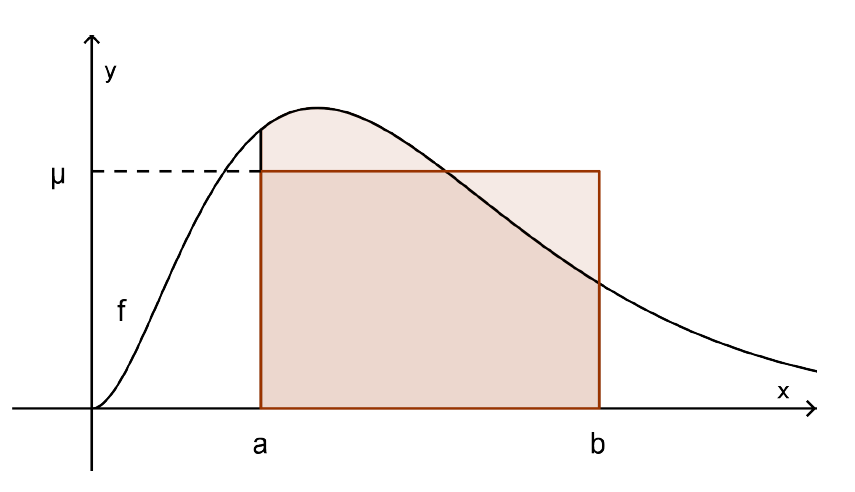
\includegraphics[width=0.4\linewidth]{Mittelwert_Grafik.png}
    \end{center}
  Definition des Mittelwert \(\mu\) der Funktion \(f(x)\) auf \([a,b]\): Höhe des Rechtecks, das
  \itemize
    \item eine Grundlinie der Länge \(b-a\) hat
    \item der Flächeninhalt des Rechteks der Fläche unter der Kurve \(f(x)\) im Intervall \([a,b]\) entspricht
	\[\mu = \frac{1}{b-a}\int_a^b{f(x)\mathrm{d}x} \]
\end{theorem}
\begin{formula}{Rotationsvolumen}\\
    \[V = \pi \int_a^b{(f(x))^2\mathrm{d}x} \]
\end{formula}
\begin{formula}{Bogenlänge}\\
    \[L=\int_a^b{\sqrt{1+(f'(x))^2}\mathrm{d}x} \]
\end{formula}
\begin{formula}{Mantelfläche}
    \[M=2\pi \int_a^b{f(x)\cdot \sqrt{1+(f'(x))^2}\mathrm{d}x} \]	
\end{formula}
\begin{theorem}{Schwerpunkt ebener Fläche}\\
  \begin{center}
  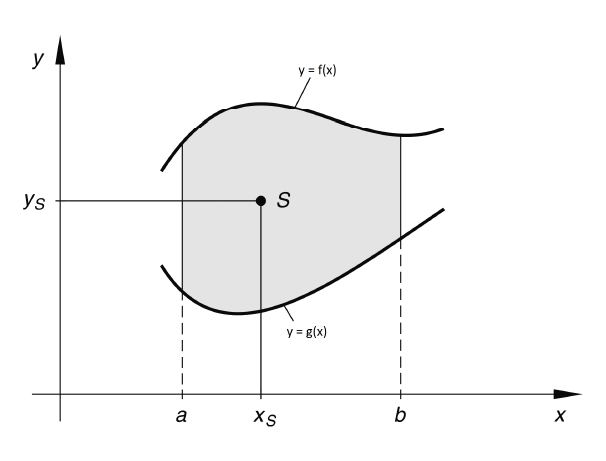
\includegraphics[width=0.4\linewidth]{Schwerpunkt_Beispiel.png}
  \end{center}
Schwerpunkt \(S=(x_s;y_s)\) einer ebenen Fläche mit Flächeninhalt A, eingegrenzt von Kurven \(y=f(x)\) und \(y=g(x)\)
sowie den Geraden \(x=a\) und \(x=b\):
\[xs = \frac{1}{A}\int_a^b{x\cdot(f(x)-g(x))\mathrm{d}x} \]
\[ys = \frac{1}{2A}\int_a^b{x\cdot(f(x)^2-g(x)^2)\mathrm{d}x} \]
Berechnen von \(A\) ebenfalls durch ein Integral:
\[A=\int_a^b{f(x)-g(x)\mathrm{d}x} \]
\end{theorem}
\begin{theorem}{Schwerpunkt Rotationskörper}\\
    Die x-Koordinate des Schwerpunkts \(S=(x_s;0;0) \) eines Rotationskörpers mit Volumen \(V\), geformt durch Rotation
    von \(y=f(x)\) zwischen \([a,b]\) um x-Achse mit \(a<b\) und \(f(x) \ge 0 \) für alle \(a \le x \le b \):
    \[x_s = \frac{\pi}{V}\int_a^b{x\cdot f(x)^2\mathrm{d}x} \]
\end{theorem}

\raggedcolumns
\columnbreak


\section{Uneigentliche Integrale}
\begin{definition}{Definition Uneigentliches Integral}
	Ein uneigentliches Integral ist ein Integral vom Type:
	\[\int_a^\infty{f(x)\mathrm{d}x}, \quad \int_{-\infty}^b{f(x)\mathrm{d}x}, \quad
	\int_{-\infty}^{\infty}{f(x)\mathrm{d}x} \quad (f(x) \: \text{ist stetig}) \]
	oder vom Typ:
	\[\int_a^b{f(x)\mathrm{d}x} \quad (f(x)\:\text{hat einen Pol im Intervall }[a,b]) \]
\end{definition}
\subsubsection{Uneigentliche Integrale erster Art}
\begin{definition}{Definition}\\
	\begin{minipage}{0.5\linewidth}
		Uneigentliche Integrale mit unendlichem Integrationsinvervall, vom Typ:
	\[I=\int_a^{\infty}{f(x)\mathrm{d}x} \]
	\end{minipage}
	\begin{minipage}{0.5\linewidth}
		\begin{center}
			Graphische Darstellung:\\
			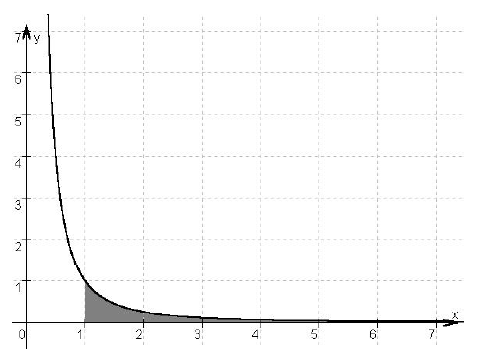
\includegraphics[width=0.6\linewidth]{Uneigentlicher_Integral_Beispiel1.png}
		\end{center}
	\end{minipage}
\end{definition}
\begin{KR}{Berechnung}
\begin{itemize}
	\item Rechnen mit endlichem Intervall \([a,\lambda] \text{ mit } \lambda \ge a \) anstelle von unendlichem
		Integral \([a,\infty) \)
		\[I(\lambda)=\int_a^{\lambda}{f(x)\mathrm{d}x} \]
	\item Das unendliche Intervall \([a,\infty) \) ergit sich aus \(\lim_{\lambda \rightarrow
		\infty}I(\lambda) \):
		\[I=\int_a^{\infty}{f(x)\mathrm{d}x}=\underset{\lambda \rightarrow \infty}{\lim}I(\lambda)=
		\underset{\lambda \rightarrow \infty}{\lim}\left(\int_a^{\lambda}{f(x)\mathrm{d}x}\right) \]
    \item Falls Grenzwert \(\underset{\lambda \rightarrow -\infty}{\lim}\) existiert, heisst das uneigentliche
        Integral \(\displaystyle\int_{a}^\infty {f(x)\mathrm{d}x}\) \(\bold{konvergent}\), andernfalls 
        \(\bold{divergent}\)
\end{itemize}
\end{KR}


\begin{KR}{Beidseitig unendliche Integrale}
\begin{itemize}
	\item Uneigentliche Integrale mit beidseitig unendlichen Integrationsinvervall:
		\[I=\int_{-\infty}^{\infty}{f(x)\mathrm{d}x}\]
	\item Einfügen einer künslichen Zwischengrenze \(c \in \mathbb{R}\\\text{typischerweise}\:c=0 \)
		\[\int_{-\infty}^{\infty}{f(x)\mathrm{d}x}=\int_{-\infty}^{c}{f(x)\mathrm{d}x}+\int_c^{\infty}
		{f(x)\mathrm{d}x} \]
	\item Beide Teilintegrale wie oben berechnen
	\item Das integral heisst \(\bold{konvergent}\) falls beide Teilintegrale konvergent sind.
\end{itemize}
\end{KR}
\subsubsection{Uneigentliche Integrale zweiter Art}
	\begin{definition}{Definition}\\
		Uneigentlich Integrale auf Interval \([a,b]\) mit einem Pol von \(f(x)\) bei \(x=a\) heisst,
		\(f(a) \rightarrow \infty\), und Stetigkeit auf \((a,b]\)
		Graphische Darstellung:
	\begin{center}
		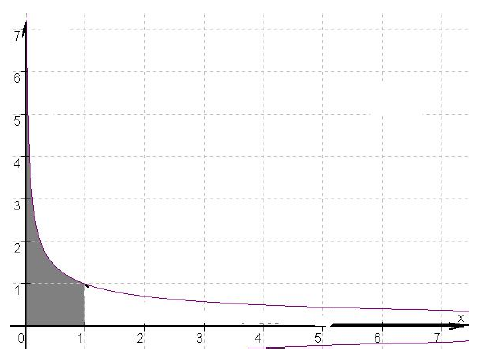
\includegraphics[width=0.4\linewidth]{Uneigentlicher_Integral_Beispiel2.png}
	\end{center}
  \end{definition}
  \begin{KR}{Berechnung}
	  \begin{itemize}
	  	
\item Statt über \([a,b]\) integrieren, integrieren über \(a+\epsilon,b\) für beliebige \(\epsilon>0\):
	\[I(\epsilon)=\int_{a+\epsilon}^b{f(x)\mathrm{d}x}\]
\item Das Integral über \([a,b]\) ergibt sich aus \(\lim_{\epsilon \rightarrow 0}I(\epsilon)\):
	\[I=\int_a^b{f(x)\mathrm{d}x}=\underset{\epsilon \rightarrow 0}{\lim}I(\epsilon)=\underset{\epsilon \rightarrow
	0}{\lim}\left(\int_{a+\epsilon}^b{f(x)\mathrm{d}x}\right) \]
\item Das Integral heisst \(\bold{konvergent}\), falls der Limes \(\lim_{\epsilon \rightarrow 0}I(\epsilon)\) existiert.
\item Diese spezielle Variante ist nötig, weil beim Integralrechnen der Integral auf dem ganzen Intervall stetig sein
	muss. Dies ist nicht der Fall wen ein Pol existiert.
\end{itemize}
  \end{KR}


  \begin{formula}{Integraltabelle}\\
    \resizebox*{1.02\linewidth}{!}{
	\def\arraystretch{1.7}
	\begin{tabular}{c|c|c}
	    Ableitung | f'(x)                          & Funktion | f(x)                          & Integral | F(x)                       \\
        \hline
	    \(0\)                                      & \(C\)                                    & \(x+C\)                               \\
        \hline
        \(1\)                                      & \(x\)                                    & \(\frac{1}{2}x^2+C\)                  \\
        \hline
        \(-\frac{1}{x^2}\)                         & \(\frac{1}{x}\)                          & \(\ln|x|+C\)                          \\
        \hline
        \(ax^{a-1}\)                               & \(x^a \: with \: a \: \in \: \mathbb{R}\) & \(\frac{x^{a+1}}{a+1}+C\)             \\
        \hline
        $x^{x} \cdot(1+\ln x) \quad x>0$          & $x^{x}$                                  &   \\
        \hline
        $\left(x^{x}\right)^{x}(x+2 x \ln (x)) \quad x>0$ & $x^{\left(x^{x}\right)}$         &  \\
        \hline  
        
        $\frac{1}{2\sqrt{x}}$                     & $\sqrt{x}$                               &  $\frac{2}{3}x^{\frac{3}{2}}$         \\
        \hline
        $\frac{1}{n} x^{\frac{1}{n}-1}$           & $\sqrt[n]{x}$                            & $\frac{n}{n+1} x^{\frac{1}{n}+1}$     \\
        \hline

        \(\ln(a)\cdot a^x\)                       & \(a^x\)                                  & \(\frac{a^x}{\ln(a)}+C\)              \\
        \hline
        $a^{b x} \cdot c \ln a$                   & $a^{b x}$                                & $\frac{1}{b \ln a} a^{b x}$             \\
        \hline
        \(e^x\)                                   & \(e^x\)                                  & \(e^x+C\)                             \\
        \hline
        \(\frac{1}{x}\)                           & \(\ln(x)\)                               & \(x\ln(x)-x+C\)                       \\
        \hline
        \(\frac{1}{x\ln(a)}\)                     & \(\log_a(x)\)                            & \(x\log_a(x)-\frac{x}{\ln(a)}+C\)     \\
        \hline
        \(\cos(x)\)                                & \(\sin(x)\)                              & \(-\cos(x)+C\)                        \\
        \hline
        \(-\sin(x)\)                               & \(\cos(x)\)                              & \(\sin(x)+C\)                         \\
        \hline
        \(1+\tan^2{(x)=\frac{1}{\cos^2{(x)}}}\)    & \(\tan(x)\)                              & \(-\ln|\cos(x)|+C\)                   \\
        \hline
        \(-1-\cot^2{(x)}=-\frac{1}{\sin^2{(x)}}\)  & \(\cot(x)\)                              & \(\ln(\sin(x))+C\)                    \\
        \hline
        \(\frac{1}{\sqrt{1-x^2}}\)                & \(\arcsin(x)\)                           & \(x\arcsin(x)+\sqrt{1-x^2}+C\)        \\
        \hline
        \(-\frac{1}{\sqrt{1-x^2}}\)               & \(\arccos(x)\)                           & \(x\arccos(x)-\sqrt{1-x^2}+C\)        \\
        \hline
        \(\frac{1}{1+x^2}\)                       & \(\arctan(x)\)                           & \(x\arctan(x)-\frac{1}{2}\ln(1+x^2)+C\)\\
        %add more here
        \hline
        $\sin ^{2}(x)$                            & $\frac{1}{2}(x-\sin (x) \cos (x))$       & $\sin (x) \cos (x) + C$                   \\
        \hline
        $\cos ^{2}(x)$                            & $\frac{1}{2}(x+\sin (x) \cos (x))$       & $\cos (x) \sin (x) + C$                   \\ 
        \hline
        $\tan ^{2}(x)$                            & $\tan (x)-x$                             & $\tan (x) + C$                            \\
        \hline
        $\cot ^{2}(x)$                            & $-\cot (x)-x$                            & $\cot (x) + C$                            \\
        \hline
        $\frac{f'(x)}{f(x)}$                      & $\ln |f(x)|$                             & $x \cdot(\ln |x|-1) + C$                 \\
        \hline
        $\frac{1}{x}(\ln x)^{n}$                  & $\frac{1}{n+1}(\ln x)^{n+1} \quad n \neq-1$ & $\frac{1}{2 n}\left(\ln x^{n}\right)^{2} \quad n \neq 0 + C$ \\
        \hline
        $\frac{1}{x \ln x}$                       & $\ln |\ln x| \quad x>0, x \neq 1$        & $\frac{1}{b \ln a} a^{b x} + C$           \\
        \hline
        $x \cdot e^{c x}$                         & $\frac{c x-1}{c^{2}} \cdot e^{c x}$      & $\frac{x^{n+1}}{n+1}\left(\ln x-\frac{1}{n+1}\right) \quad n \neq-1 + C$ \\
        \hline
        $x^{n} \ln x$                             & $\ln (\cosh (x))$                        & $\ln |f(x)| + C$                          \\
        \hline
        $\sin (x) \cos (x)$                       & $\frac{\sin^2(x)}{2} $                &\\
        \hline
        $\frac{-f^{\prime}(x)}{(f(x))^{2}}$       & $\frac{1}{f(x)}$                         & \\
        \hline
        $(a x+b)^{n}$                             & $\frac{1}{a \cdot(n+1)}(a x+b)^{n+1}$   & \\
        \hline
	\end{tabular}
    }
\end{formula}

\begin{KR}{Trick Gerade/Ungerade bei Integralen}\\
    Für ungerade Funktionen gilt $\int_{-a}^{+a} f(x) \dif x = 0$.
    \begin{itemize}
        \item Summe/Komposition: ungerade und ungerade $\rightarrow$ ungerade
        \item Produkt/Quotient: ungerade und gerade $\rightarrow$ ungerade
        \item Ableitung: gerade $\longrightarrow$ ungerade
    \end{itemize}
    Bsp ungerade: $f(x)$ = $-x$, $x$, $sin(x)$, $tan(x)$, Polynomfunktionen mit ungeradem Exponent\\
    gerade: $1$, $x^2$, $cos(x)$, $sec(x)$, Polynomf. mit geradem Exponent\\
    gerade und ungerade!! $f(x) = 0$
\end{KR}
	\raggedcolumns
	\pagebreak
	\section{Differentialrechnung}




   

\subsubsection{Differentialquotient und Ableitung}


\begin{definition}{Sekanten-Steigung und Differentialquotient}\\
    Sei $f$ eine Funktion und $\left[x_{0}, x_{0}+h\right]$ ein Intervall im Definitionsbereich von $f$. Der Quotient
    
    $$\frac{\Delta f}{\Delta \mathrm{x}}=\frac{f\left(x_{0}+h\right)-f\left(x_{0}\right)}{h}$$
    
    heisst Differentialquotient von $f$.
\end{definition}


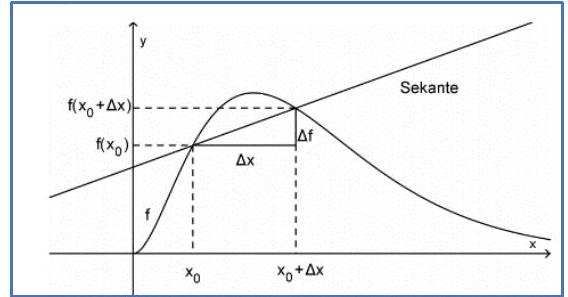
\includegraphics[scale=0.3]{2024_01_20_7bfda6c084929ccc01ffg-03.jpg}


\begin{definition}{Differenzierbarkeit}\\
    $f$ ist in $x_0$ \emph{differenzierbar}, falls der Grenzwert $\lim_{x \to x_0} \frac{f(x) -f(x_0)}{x -x_0}$
    existiert.\\
    Ist dies der Fall, wird der Grenzwert mit $f'(x)$ bezeichnet.
        $$
        f'(x_0) = \lim_{h \to 0}\frac{\Delta f}{\Delta \mathrm{x}} = \lim_{h \to 0}\frac{f(x_0 + h) -f (x_0)}{h}
        $$
    Den Grenzwert selbst bezeichnet man als Ableitung.
    \tcblower 
    \small
    Vereinfacht: Eine Funktion ist differenzierbar, falls die Kurve keine Knicke macht.
\end{definition}

\begin{formula}{Tangentengleichung}
    $
    y=f^{\prime}\left(x_{0}\right) \cdot\left(x-x_{0}\right)+f\left(x_{0}\right)
    $
\end{formula}

\begin{definition}{Stetige Differenzierbarkeit}
	Eine Funktion ist stetig differenzierbar, wenn sie differenzierbar ist und ihre Ableitungsfunktion stetig ist.
\end{definition}


\begin{definition}{n-fache Differenzierbarkeit}
	\begin{enumerate}
		\item Für $n \geq 2$ ist $f$ \emph{$n$-mal differenzierbar} in $D$ falls $f^{n-1}$ in $D$ differenzierbar ist. Dann ist $f^{(n)} \coloneqq \left(f^{(n-1)}\right)'$ und nennnt sich die $n$-te Ableitung von $f$.
		\item Die Funktion $f$ ist \emph{$n$-mal stetig differenzierbar} in $D$, falls sie $n$-mal differenzierbar ist und falls $f^{(n)}$ in $D$ stetig ist.
		\item Die Funktion $f$ ist in $D$ \emph{glatt}, falls sie $\forall n \geq 1$, $n$-mal differenzierbar ist. 
	\end{enumerate}
\end{definition}


\begin{itemize}
	\item $\exp$, $\sin$, $\cos$, $\sinh$, $\cosh$, $\tanh$ sind glatt auf $\R$
	\item Alle Polynome sind auf ganz $\R$ glatt
	\item $\ln : ]0, + \infty[ \to \R$ ist glatt
\end{itemize}

\begin{theorem}{Rechnen mit höheren Ableitungen}\\
	Sei $D \subseteq \R$, $n \geq 1$ und $f,g \to \R$ $n$-mal differenzierbar in $D$.
	\begin{enumerate}
		\item $f+g$ ist $n$-mal differenzierbar und $(f + g)^{(n)} = f^{(n)} + g^{(n)}$
		\item $f \cdot g$ ist $n$-mal differenzierbar und\\ $(f \cdot g)^{(n)} = \sum_{k=0}^n \binom{n}{k} f^{(k)} g^{(n-k)}$.
        \item $\frac{f}{g}$ ist n-mal differenzierbar falls $g(x) \neq 0, \forall x \in D$
        \item $(g \circ f)$ ist n-mal differenzierbar
	\end{enumerate}
\end{theorem}





\begin{concept}{Ableitungsregeln}
    Seien $f,g: D \to \R$  differenzierbar. Dann gelten:
    \begin{itemize}
        \item Summe/Differenz: $(f + g)'(x) = f'(x) + g'(x)$
        \item Faktor: $f(x)=a\cdot g(x) \rightarrow f'(x)=a \cdot g'(x) $
        \item Produkt: $(f \cdot g)'(x) = f'(x)g(x) + f(x)g'(x)$
        \item Quotient: $\left(\frac{f}{g}\right)'(x) = \frac{f'(x) g(x) - f(x) g'(x)}{g(x)^2}$
        \item Kettenregel: $(g \circ f)' (x) = g'(f(x)) f'(x)$
        \item Umkehrfunktion: $\left(f^{-1}\right)'(y_0) = \frac{1}{f'(x)}$
        \item Potenz/Logarithmus 1: 
        $(a^{f(x)})' = ln(a) \cdot a^{f(x)} \cdot f'(x)$

        \resizebox{\linewidth}{!}{
            $(f(x)^{g(x)})' = f(x)^{g(x)} \cdot (ln(f(x)) \cdot g(x))' =  f(x)^{g(x)} \cdot (ln(f(x)) \cdot g(x) \cdot \frac{f'(x)}{f(x)})$
            }
    \end{itemize}
    Bem. Für gerade $k$ gilt $\cosh (x)^{(k)}=\cosh (x)$ und für ungerade $k$ gilt $\cosh (x)^{(k)}=\sinh (x)$, analoges gilt für $\sinh$.
\end{concept}

 \begin{KR}{Differentialrechnung Tricks}
        \begin{itemize}
      \item Überall differenzierbar: Einheitliche Tangente (Ableitung 0 setzen) und dh: Grenzwerte müssen denselben Wert ergeben
      \item Zwei Funktionskurven berühren sich (aww): bedeutet dass sie an Stelle x0 gleichen Funktionswert und gleiche Ableitung haben
      \item Tangente bestimmen (Linearisierung): $f\left(x_{0}\right)+f^{\prime}\left(x_{0}\right)\left(x-x_{0}\right)$
    \end{itemize}
    \end{KR}

\begin{formula}{Grundfunktionen der Ableitung}
    \begin{itemize}
        \item Potenz 
    \end{itemize}
    \vspace{-3mm}
    $$f(x)=x^{n} \quad f^{\prime}(x)=n \cdot x^{n-1}$$
    \begin{itemize}
      \item Exponent
    \end{itemize}
    \vspace{-3mm}
    $$
    \begin{array}{ll}
    f(x)=a^{x} & f^{\prime}(x)=a^{x} \cdot \ln (a) \\
    f(x)=e^{x} & f^{\prime}(x)=e^{x}
    \end{array}
    $$
    
    \begin{itemize}
      \item Logarithmus
    \end{itemize}
    \vspace{-3mm}
    $$
    \begin{array}{ll}
    f(x)=\ln (x) & f^{\prime}(x)=\frac{1}{x} \\
    f(x)=\log _{a}(x) & f^{\prime}(x)=\frac{1}{\ln (a) \cdot x}
    \end{array}
    $$
\end{formula}


\begin{formula}{Ableitungen von geometrischen Funktionen}
    $$
    \arctan ^{\prime}(x) =\frac{1}{1+x^{2}}, 
    \arcsin ^{\prime}(x) =\frac{1}{\sqrt{1-x^{2}}}, 
    \arccos ^{\prime}(x) =\frac{1}{\sqrt{1+x^{2}}}
    $$

    $$
    \begin{array}{ll}
    f(x)=\tan (x) & f^{\prime}(x)=1+\tan ^{2}(x)=\frac{1}{\cos ^{2}(x)} \\
    f(x)=\cot (x) & f^{\prime}(x)=-1-\cot ^{2}(x)=-\frac{1}{\sin ^{2}(x)}
    \end{array}
    $$
\end{formula}

\begin{definition}[breakable]{Monotonie}\\
    Sei $y=f(x)$ eine differenzierbare Funktion in $D$ mit $x_{0} \in D$.
    \begin{itemize}
        \item $f'( x_{0}) = 0$ $ \Rightarrow$   $f$ konstant, bzw. horizontale Tangente
        \item $f'( x_{0}) > 0 $ $ \Rightarrow$  $f$  streng monoton wachsend.
        \item $f'( x_{0}) < 0 $ $ \Rightarrow$ $f$ streng monoton fallend.
    \end{itemize}
\end{definition}
\begin{theorem}{Krümmung}\\
    Zusammenhang zwischen 2. Ableitung und Krümmung:
    \begin{itemize}
      \item $f^{\prime \prime}\left(x_{0}\right)>0$ Konvex (Nach links/oben gekrümmt)
      \item $f^{\prime \prime}\left(x_{0}\right)<0$ Konkav (Nach rechts/unten gekrümmt)
      \item $f^{\prime \prime}\left(x_{0}\right)=0$ Keine eindeutige Krümmung
    \end{itemize}
    Bmk: Die Summe zweier konvexer Funktionen ist konvex. (konkav analog)
\end{theorem}

\begin{definition}{Wende- und Sattelpunkte}
    Als Wendepunkte werden Punkte bezeichnet bei denen sich der «Drehsinn» ändert. Wendepunkte mit horizontaler Tangente werden als Sattelpunkte oder Terrassenpunkte bezeichnet\\

Wendetangente: Tangente an einem Wendepunkt
\end{definition}



\begin{KR}{Berechnung Wendetangente}
    Ermittlung durch Lösen der Gleichung $f^{\prime \prime}(x)=0 \rightarrow x_{0}$.\\
    Bedingungen:\\
    Sei $y=f(x)$ dreimal differenzierbar

\begin{itemize}
  \item $f^{\prime \prime}\left(x_{0}\right)=0$
  \item $f^{(3)}\left(x_{0}\right) \neq 0 \quad \rightarrow$ Wendepunkt
  \item Falls zusätzlich $f^{\prime}\left(x_{0}\right)=0 \quad \rightarrow$ Sattelpunkt
\end{itemize}
    
\end{KR}

\begin{concept}{Allgemeines Kriterium}\\
    Sei $f(x)$ eine genügend oft differenzierbare Funktion

\begin{itemize}
  \item $f^{\prime}\left(x_{0}\right)=0$
\end{itemize}

Sei $n$ die Ordnung der ersten nicht verschwindenden Ableitung von $f(x)$ an der Stelle $x_{0}$:

\begin{itemize}
  \item $f^{\prime}\left(x_{0}\right)=f^{\prime \prime}\left(x_{0}\right)=\cdots=f^{(n-1)}\left(x_{0}\right)=0$
  \item $f^{(n)}\left(x_{0}\right) \neq 0$
\end{itemize}

Schlussfolgerungen:
\begin{itemize}
    \item Wenn $n$ gerade, dann gibt es ein relatives Extremum $\left(f^{(n)}\left(x_{0}\right) \neq 0\right)$
    \item Wenn $n$ ungerade, dann hat $f(x)$ an der Stelle $x_{0}$ einen Wendepunkt und damit einen Sattelpunkt
\end{itemize}
\end{concept}

\begin{KR}{Vorgehen Wende- und Sattelpunkte}
    \begin{enumerate}
  \item Erste und zweite Ableitung

  \item Wendepunkt bestimmen

\end{enumerate}

\begin{itemize}
  \item $f^{\prime \prime}\left(x_{0}\right)=0 \rightarrow x_{0}$
  \item $f^{(3)}\left(x_{0}\right) \neq 0$
\end{itemize}

\begin{enumerate}
  \setcounter{enumi}{2}
  \item Sattelpunkte bestimmen
\end{enumerate}

\begin{itemize}
  \item $f^{\prime}\left(x_{0}\right)=0$
  \item $f^{\prime \prime}\left(x_{0}\right)=0$
  \item ...
  \item $f^{(n)}\left(x_{0}\right) \neq 0$
  \item Gerade $\rightarrow$ relatives Extremum
  \item Ungerade $\rightarrow$ Sattelpunkt
\end{itemize}

\begin{enumerate}
  \setcounter{enumi}{3}
  \item $x_{0}$ in ursprüngliche Gleichung einsetzen
\end{enumerate}
\end{KR}


\begin{definition}{Relative Extrema}
    \begin{itemize}
      \item Relative Extremal-Stelle $x_0$ $\quad \Longrightarrow \quad$ Minimal-/Maximalstelle
    
      \item Relatives Extremum $y_0$ $\quad \Longrightarrow \quad$ Maximum/Minimum
    
      \item Relativer Extremal-Punkt $P_0 = (x_0, y_0)$ $\quad \Longrightarrow \quad$ Hoch-/Tiefpunkt
    
    \end{itemize}
\end{definition}

%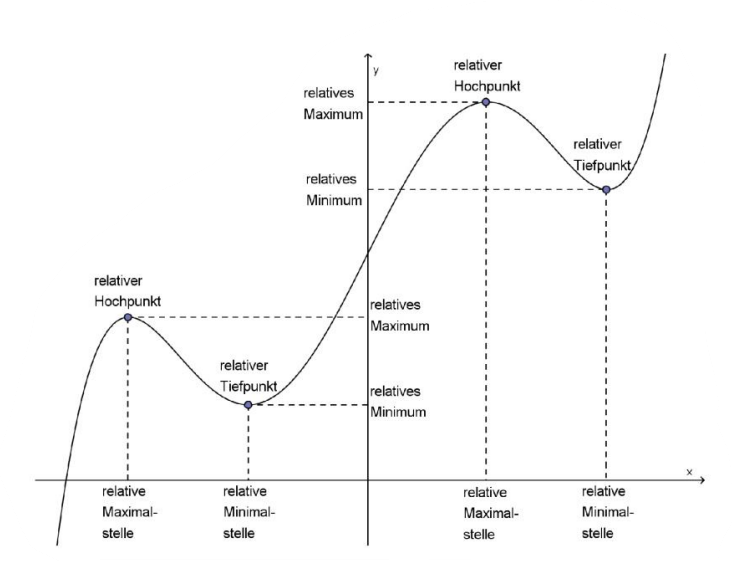
\includegraphics[scale=0.45]{Analysis1/zsf/Images/Differential/relative maxima.png}

\begin{KR}{Vorgehen relative Extrema} von $f(x) = y$:
    \begin{enumerate}
	\item Bestimme $f'(x)$ (Erste Ableitung)
	\item Bestimme NST von $f'(x)$\\
		$f'(x) = 0$ $ \Rightarrow$ $x$ lokales Extremum
	\item Bestimme $f''(x)$ (Zweite Ableitung)
		\begin{itemize}
			\item $f''(x) = 0$ $ \Rightarrow$ siehe Vorgehen Wende- und Sattelpunkte
			\item $f''(x) < 0$ $ \Rightarrow$ relatives Maximum
			\item $f''(x) > 0$ $ \Rightarrow$ relatives Minimum
		\end{itemize}
    \item In Gleichung f(x) = y einsetzen
        \begin{itemize}
            \item Hochpunkt/Tiefpunkt = $P(x, y)$
        \end{itemize}
\end{enumerate}
\end{KR}


\begin{formula}{Quadratische Funktionen}
$y=a x^{2}+b x+c$

    Nullstellen
    
    \begin{itemize}
      \item $y=a\left(x-x_{1}\right)\left(x-x_{2}\right)$
      \item $x_{0}=\frac{-b \pm \sqrt{b^{2}-4 a c}}{2 a}$
    \end{itemize}
    
    Scheitelpunkt
    
    \begin{itemize}
      \item $y=a\left(x-x_{0}\right)^{2}+y_{0}$
      \item $\mathrm{S}=\left(-\frac{b}{2 a}, \frac{4 a c-b^{2}}{4 a}\right)$
    \end{itemize}
\end{formula}
































	\raggedcolumns
	\pagebreak
	\section{Differentialgleichungen}

\begin{definition}{Differentialgleichung}
  \(n\)-ter Ordnung ist ein Gleichung von der Form:
      \[F(x,y,y',y'',\ldots,y^{(n)})=0\]
  \begin{itemize}
    \item Eine Differentialgleichung 
      für eine gesuchte Funktion \(y=y(x)\), in der Ableitungen von \(y(x)\) bis zur \(n\)-ten Ordnung auftreten.
    \item Falls die DGL nach \(y^{(n)}\) aufgelöst ist, nennt man sie explizit, ansonsten implizit.
      Oft können implizite DGL durch einfaches Umformen in explizite DGL umgewandelt werden.
  \end{itemize}
\end{definition}

\begin{definition}{Arten von DGL}
  \begin{itemize}
    \item \emph{Separierbar:} falls \(F(x,y)\) als Produkt eines \(x\)- und eines \(y\)-Anteils geschrieben
      werden kann, d.h. es hat die Form:
      \[y'=g(x)\cdot h(y)\]
    \item \emph{Autonom:} falls \(F(x,y)\) nur von \(y\) abhängt, d.h. es hat die Form:
      \[y'=f(y)\]
    \item \emph{Linear:} falls die Variabel welche abgeleitet wird, nur in der ersten Potenz vorkommt und nicht
      multipliziert miteinander oder mit der unabhängigen Variabel wird.
  \end{itemize}
\end{definition}

\begin{KR}{Lösen von Separierbaren DGL}
  \begin{center}
    DGL:
      $\frac{\mathrm{d}y}{\mathrm{d}x}=g(x)\cdot h(y)$\\
      \vspace{1mm}
      $\rightarrow$ Falls \(h(y_0)=0\), ist \(y=y_0\) eine Lösung der DGL.
  \end{center}
  \begin{itemize}
    \item Trennung aller \(x\)- und \(y\)-Terme:
    $\frac{1}{h(y)}\cdot \mathrm{d}y=g(x)\cdot \mathrm{d}x$
    \item Integration auf beiden Seiten:
    $\int{\frac{1}{h(y)}\mathrm{d}y}=\int{g(x)\mathrm{d}x}$
    \end{itemize}
  Auflösen nach \(y\), Anfangsbedingungen einsetzen:
      \[\int_{y_0}^{y}{\frac{1}{h(s)}\mathrm{d}s}=\int_{x_0}^{x}{g(t)\mathrm{d}t}\]
\end{KR}

\begin{definition}{Homogenität von DGL}
  \begin{itemize}
    \item Homogene DGL: \(F(x,y,y',y'',\ldots,y^{(n)})=0\)
    \item Inhomogene DGL: \(F(x,y,y',y'',\ldots,y^{(n)})=g(x)\)
    \begin{itemize}
      \item \(g(x)\) ist die Störfunktion
    \end{itemize}
  \end{itemize}
\end{definition}

\begin{formula}{Allgemeine Lösung der inhomogenen DGL}
  $y'+f(x)y=g(x)$
      ist gegeben durch:
      \[y=e^{-F(x)}\cdot \int{g(x)e^{F(x)}\mathrm{d}x}\]
      wobei \(F(x)\) eine Stammfunktion von \(f(x)\) ist.

\end{formula}

\begin{definition}{Anfangswertproblem} DGL mit Anfangsbedingung\\
  Anfangswertproblem \(n\)-ter Ordnung:
      \[\left\{\begin{tabular}{rcl}
	  \( F(x,y,y',y'',\ldots,y^{(n)})\)&\(=\)&\(0,\;(x,y,\ldots,y^{(n)})\in \Omega\)\\
	  \(y(x_0)\)&\(=\)&\(y_0\)\\
	  \(y'(x_0)\)&\(=\)&\(y_1\)\\
		\(\) &\(\vdots\)&\(\)\\
	 \( y^{n-1}(x_0)\)&\(=\)&\( y_{n-1}\)
      \end{tabular}\right.\]
      Anfangswertproblem für explizite DGL 1. Ordnung:
      \[\left\{\begin{tabular}{rcl}
	  \(y'\)&\(=\)&\(G(x,y),\quad (x,y,y')\in \Omega\subseteq\mathbb{R}\times\mathbb{R}^2\)\\
	  \(y(x_0)\)&\(=\)&\(y_0\)
      \end{tabular}\right.\]
  \begin{itemize}
    \item Allgemeine Lösung: Menge aller Lösungen einer DGL
    \item Spezielle/partikuläre Lösung: Lösung eines Anfangswertproblems
  \end{itemize}
\end{definition}

\begin{KR}{Lösung von Anfangswertproblemen mit seperiarbaren DGL}
  \begin{itemize}
    \item Sind \(g(x)\) und \(h(y)\) stetige Funktionen und \((x_0,y_0)\in \mathbb{R}^2\) mit \(h(y_0)\neq 0\), hat das
      Anfangswertproblem:
      \[\left\{\begin{tabular}{rcl}
	  \(y'\)&\(=\)&\(g(x)h(y)\)\\
	  \(y(x_0)\)&\(=\)&\(y_0\)\\
      \end{tabular}\right.\]
      genau eine Lösung. Sie kann gefunden werden, indem beide Seiten von 
      \[\int_{y_0}^{y}{\frac{1}{h(s)}\mathrm{d}s}=\int_{x_0}^{x}{g(t)\mathrm{d}t}\]
      berechnet werden und nach \(y\) aufgelöst werden.
  \end{itemize}
\end{KR}

\paragraph{Richtungsfeder}
\begin{definition}{Richtungsfeld} geometrisches Verständnis von expliziten DGL 1. Ordnung, d.h. DGL der Form:
  $y'=f(x,y)$
  %\vspace{3mm}  \\
  \begin{minipage}{0.45\linewidth}
    \begin{center}
    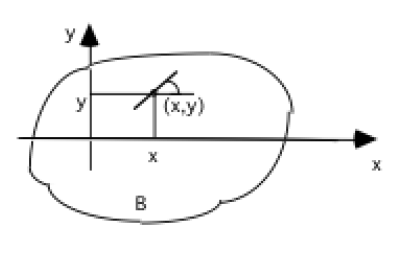
\includegraphics[width=0.8\linewidth]{Richtungsfeld.png}
    \end{center}
  \end{minipage}
  \hspace{3mm}
  \begin{minipage}{0.45\linewidth}
    \begin{center}
    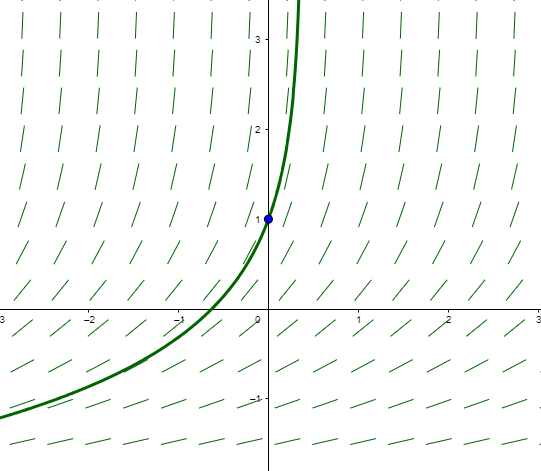
\includegraphics[width=0.8\linewidth]{RichtungsfeldKurve.png}
    \end{center}
  \end{minipage}

  \begin{minipage}{0.45\linewidth}
    \(f(x,y)\) gibt also die Steigung der Lösungskurve am Punkt \((x,y)\) an
  \end{minipage}
  \hspace{3mm}
  \begin{minipage}{0.45\linewidth}
    Jeder Punkt ist somit die Tangente einer spezifischen Lösungskurve
  \end{minipage}
\end{definition}

\begin{definition}{Richtungsfelder von Speziellen DGL}\\
  \begin{minipage}{0.58\linewidth}
    Unbestimmtes Integral: \(y'=f(x)\)\\ das Richtungsfeld ist unabhängig von \(y\) die verschiedenen Lösungen
      unterscheiden sich nur durch eine verschiebung in \(y\)-Richtung durch die Konstante \(C\).
  \end{minipage}
  \begin{minipage}{0.4\linewidth}
    \begin{center}
      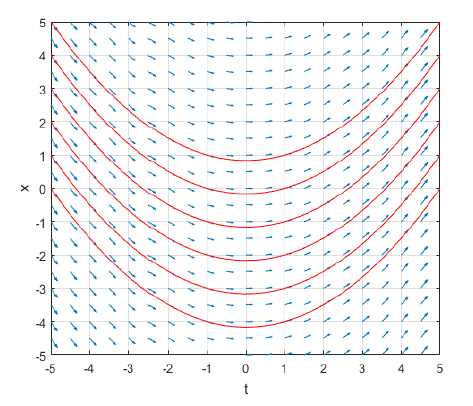
\includegraphics[width=1\linewidth]{UnbestimmtesIntegral.png}
      \end{center}
  \end{minipage}
  \begin{minipage}{0.58\linewidth}
    Autonome DGL:\(y'=f(y)\)\\ das Richtungsfeld ist unabhängig von \(x\) die Verschiedenen Lösungen gehen durch
    Verschiebung in \(x\)-Richtung in einander über.
  \end{minipage}
  \begin{minipage}{0.4\linewidth}
    \begin{center}
      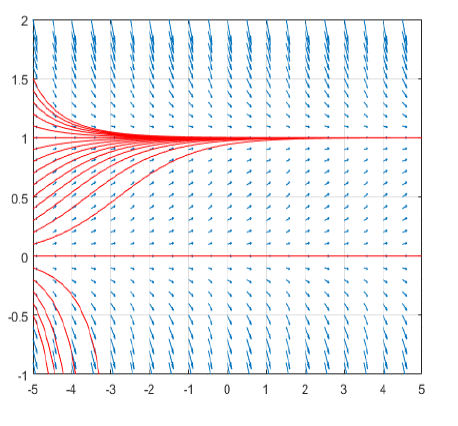
\includegraphics[width=1\linewidth]{AutonomeDGL.png}
      \end{center}
  \end{minipage}
\end{definition}






\paragraph{Numerische Verfahren}
\begin{definition}{Eulerverfahren}
  Gleichung einer beliebigen Geraden mit Steigung \(m\) am Punkt \((x_k,y_k)\):
      \[y=y_k+m\cdot(x-x_k)\]
    \begin{minipage}{0.5\linewidth}
      DGL am Punkt \((x_k,y_k)\):
      \[y=y_k+f(x_k,y_k)\cdot (x-x_k)\]
    \end{minipage}
    \begin{minipage}{0.45\linewidth}
      \begin{center}
        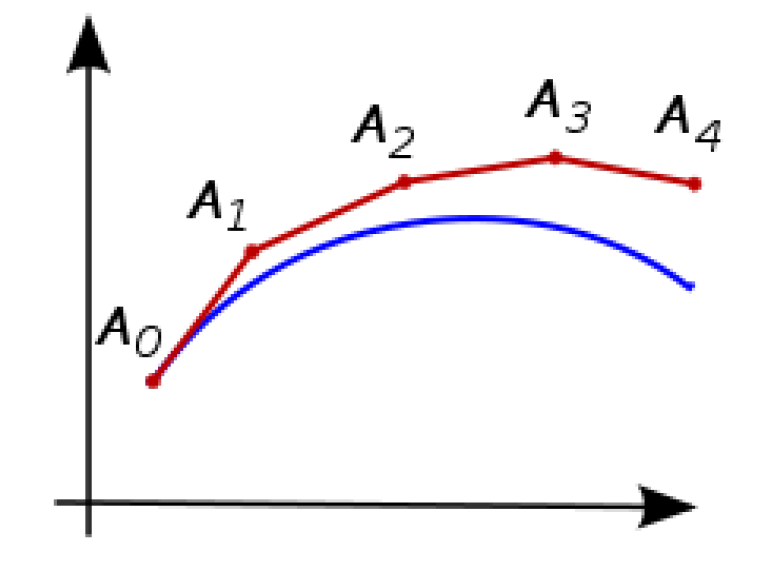
\includegraphics[width=0.7\linewidth]{Newtonverfahren.png}
        \end{center}
    \end{minipage}
  \begin{itemize}

    \item Für \(k=0 \text{ und } x=x_0\):
      \[\underbrace{y_1}_{\approx y(x_1)}=y_0+f(x_0,y_0)\cdot\underbrace{(x_1-x_0)}_{=h}\]
    \item Algorithmus für beliebige \(k\):
      \[\left\{\begin{tabular}{rcl}
	  \(x_k\)&\(=\)&\(x_0+k\cdot h\)\\
	  \(y_{k+1}\)&\(=\)&\(y_k+h\cdot f(x_k,y_k)\)
	\end{tabular}
      \right.\]
  \end{itemize}
  Problem: Die Steigung wird nur am linken Ende des Intervalls berücksichtigt!
    \\ $\Rightarrow$ Lösung: Verbesserte numerische Verfahren!
\end{definition}

	\raggedcolumns
	\pagebreak
	%Linear Algebra
	

\section{Vektorgeometrie}

\begin{definition}{Vektor}
    Objekt, das Betrag und Richtung hat.
    \begin{itemize}
        \item $\overrightarrow{0} = $ Nullvektor (Betrag = 0, einziger Vektor ohne Richtung)
        \item $\overrightarrow{e} = $ Einheitsvektor (Betrag = 1), evtl. mit Index $\vec{e_a}$
        \item $\vec{PQ}=$ Vektor, der den Punkt $P$ in $Q$ verschiebt
        \item $\vec{a} = \vec{b} \Leftrightarrow \abs{\vec{a}} = \abs{\vec{b}}$ und $\vec{a} \parallel \vec{b}$ (selber Betrag und Richtung)
    \end{itemize}
    Es wird zwischen \textit{Orts-} und \textit{Richtungsvektoren} unterschieden.
\end{definition}

\begin{minipage}{0.6\linewidth}
    \begin{definition}{Gegenvektor}
        $-\vec{a}$ ist parallel zu $\vec{a}$, hat denselben Betrag,
        aber entgegengesetzte Richtung. 
    \end{definition}
    \end{minipage}
    \begin{minipage}{0.25\linewidth}
        {\small
        $$-\overrightarrow{a} = \begin{pmatrix}
            -a_x \\
            -a_y
            \end{pmatrix}$$}
    \end{minipage}
    \begin{minipage}{0.13\linewidth}
        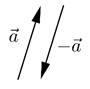
\includegraphics[width=0.8\linewidth]{vec-gegen.png}
    \end{minipage}

\begin{definition}{Länge/Betrag eines Vektors}
    $\abs{\vec{a}}=\sqrt{a_1^2+a_2^2+\cdots+a_n^2}$
\end{definition}

\begin{formula}{Einheitsvektor/Normierung}
    {\large
    $\vec{e_a}=\frac{1}{a}\cdot\vec{a} \quad = \quad \frac{\overrightarrow{a}}{|\overrightarrow{a}|}$}

    Der Vektor $\vec{e_a}$ wird als \textbf{Einheitsvektor oder auch normiert} bezeichnet 
    und der Übergang von $\vec{a}$ nach $\vec{e_a}$ heisst \textbf{Normierung}.
\end{formula}



\begin{definition}{Orthogonal (Senkrecht)} $\overrightarrow{a} \cdot \overrightarrow{b} = 0 \rightarrow \text{ orthogonal}$

    $\vec{a}$ und $\vec{b}$ sind orthogonal, wenn der Winkel zwischen ihnen 90° beträgt
\end{definition}

\begin{definition}{Normalenvektor}
    Ein Normalenvektor, der orthogonal zu einer Ebene $E$ ist, heisst \textit{Normalenvektor} von $E$.
    Eine Koordinatendarstellung einer Ebene $E$ heisst normiert, wenn gilt: $\vec{n}=1$.
\end{definition}



\raggedcolumns

\paragraph*{Rechnen mit Vektoren}

\begin{minipage}{0.5\linewidth}
    \begin{formula}{Vektoraddition}\\
        $\overrightarrow{a} + \overrightarrow{b} = \begin{pmatrix} a_x + b_x\\ a_y + b_y \end{pmatrix}$
    \end{formula}
\end{minipage}
\begin{minipage}{0.5\linewidth}
\begin{formula}{Skalarmultiplikation}\\
    $\lambda \cdot \overrightarrow{a} = \begin{pmatrix}
    \lambda \cdot a_x \\
    \lambda \cdot a_y
    \end{pmatrix}$
\end{formula}
\end{minipage}

\raggedcolumns

\begin{formula}{Skalarprodukt} 
    $\overrightarrow{a} \cdot \overrightarrow{b} = a_x \cdot b_x + a_y \cdot b_y = |\overrightarrow{a}| \cdot |\overrightarrow{b}| \cdot \cos(\varphi)$
\end{formula}

\begin{formula}{Winkelberechnung} {\small $\varphi$ = Winkel zwischen $\vec{a}$ und $\vec{b}$ ($0\le\phi\le\pi$)}
    $$\cos(\varphi) = \frac{\overrightarrow{a} \cdot \overrightarrow{b}}{|\overrightarrow{a}| \cdot |\overrightarrow{b}|} = \frac{a_x b_x + a_y b_y}{\sqrt{a_x^2 + a_y^2} \cdot \sqrt{b_x^2 + b_y^2}  } $$
\end{formula}


\begin{minipage}{0.55\linewidth}
\begin{concept}{Winkel und Skalarprodukt}\\
    Seien $\vec{a}$ und $\vec{b}$ zwei Vektoren und $\varphi$ der eingeschlossene Winkel, 
    $0\leq\varphi\leq\pi$, dann gilt:
\end{concept}
\end{minipage}
\begin{minipage}{0.35\linewidth}
    $\varphi<\frac{\pi}{2},\, \text{ wenn } \vec{a}\cdot\vec{b} > 0 \\  
    \varphi>\frac{\pi}{2},\, \text{ wenn } \vec{a}\cdot\vec{b} < 0 \\   
    \varphi=\frac{\pi}{2},\, \text{ wenn } \vec{a}\cdot\vec{b} = 0 $
\end{minipage}

\begin{theorem}{Eigenschaften des Skalarprodukts}\\ Für beliebige Vektoren $\vec{a}$, $\vec{b}$, $\vec{c}$ und Skalaren $\lambda\in\R$ gilt:
    \begin{itemize}
        \item $\vec{a}\cdot\vec{a}=\abs{\vec{a}}^2$
        \item $(-\lambda)\cdot\vec{a}=-(\lambda\cdot\vec{a})=\lambda\cdot(-\vec{a})$
        \item Kommutativ-Gesetz: $\vec{a}\cdot\vec{b}=\vec{b}\cdot\vec{a}$
        \item Distributiv-Gesetze: $\vec{a}\cdot(\vec{b}+\vec{c})=\vec{a}\cdot\vec{b}+\vec{a}\cdot\vec{c}$ und $(\vec{a}+\vec{a})\cdot\vec{c}=\vec{a}\cdot\vec{c}+\vec{b}\cdot\vec{c}$
        \item Gemischtes Assoziativ-Gesetz: $\lambda\cdot(\vec{a}\cdot\vec{b})=(\lambda\cdot\vec{a})\cdot\vec{b}=\vec{a}\cdot(\lambda\cdot\vec{b})$
    \end{itemize} 
\end{theorem}

\begin{minipage}{0.8\linewidth}
\begin{formula}{Kreuzprodukt} {\small $\overrightarrow{a} \times \overrightarrow{b}$ ist orthogonal zu $\overrightarrow{a}$ und $\overrightarrow{b}$
        $$\overrightarrow{a} \times \overrightarrow{b} = \left(\begin{array}{ccc}
            a_y \cdot b_z &-& a_z \cdot b_y \\
            a_z \cdot b_x &-& a_x \cdot b_z \\
            a_x \cdot b_y &-& a_y \cdot b_x
            \end{array}\right)$$
    \vspace{2mm}
    $|\overrightarrow{a} \times \overrightarrow{b}| = |\overrightarrow{a}| \cdot |\overrightarrow{b}| \cdot \sin(\varphi) 
        \quad \quad \quad \overrightarrow{a} \times \overrightarrow{b} \neq \overrightarrow{b} \times \overrightarrow{a}$
    
        \vspace{1mm}

        Für $\R^2$ gilt: $\overrightarrow{a} \times \overrightarrow{b} = a_x \cdot b_y - a_y \cdot b_x$
        }
\end{formula}
\end{minipage}
\begin{minipage}{0.19\linewidth}
    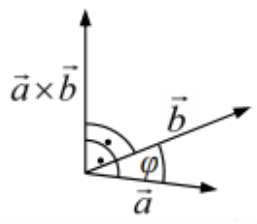
\includegraphics[width=1\linewidth]{vektorprodukt.png}
\end{minipage}  

\begin{theorem}{Eigenschaften des Kreuzprodukts} auch genannt Vektorprodukt\\
    Für beliebige Vektoren $\vec{a}$, $\vec{b}$, $\vec{c}$ und Skalaren $\lambda\in\R$ gilt:
    \begin{itemize}
        \item $\vec{a}\times\vec{a}=\vec{0}$
        \item Antikommutativ-Gesetz: $\vec{a}\times\vec{b}=-(\vec{b}\times\vec{a})$
        \item Distributiv-Gesetz: $\vec{a}\times(\vec{b}+\vec{c})=\vec{a}\times\vec{b}+\vec{a}\times\vec{c}$
        \item Gemischtes Assoziativ-Gesetz:
            $\lambda\cdot(\vec{a}\times\vec{b})=(\lambda\cdot\vec{a})\times\vec{b}=\vec{a}\times(\lambda\cdot\vec{b})$ 
    \end{itemize}
    \textcolor{pink}{$\vec{a}\times(\vec{b}\times\vec{c})\ne(\vec{a}\times\vec{b})\times\vec{c}$!!}
\end{theorem}

\begin{formula}{Fläche des aufgespannten Parallelogramms} = $\vec{a}\times\vec{b}$\\
    \begin{minipage}{0.6\linewidth}
    $$h = |\overrightarrow{b}| \cdot \sin(\varphi)$$
    $$A = |\overrightarrow{a}| \cdot h = |\overrightarrow{a} \times \overrightarrow{b}| = |\overrightarrow{a}| \cdot |\overrightarrow{b}| \cdot \sin(\varphi)$$
    \end{minipage}
    \hspace{3mm}
    \begin{minipage}{0.35\linewidth}
        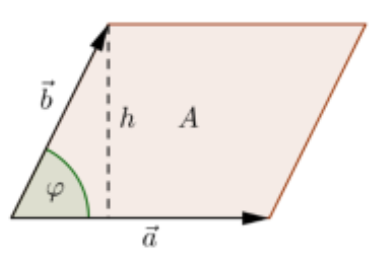
\includegraphics[width=0.7\linewidth]{parallelogramm.png}
    \end{minipage}
\end{formula}



\begin{minipage}{0.7\linewidth}
    \begin{formula}{Orthogonal Projektion}von $\overrightarrow{b}$ auf $\overrightarrow{a}$
            $$\vec{b}_a=\frac{\vec{a}\cdot\vec{b}}{\abs{\vec{a}}^2}\cdot\vec{a}   
            \text{ und }
            \abs{\vec{b}}_a=\frac{\abs{\vec{a}\cdot\vec{b}}}{\abs{\vec{a}}}  $$
    \end{formula}
\end{minipage}
    \begin{minipage}{0.25\linewidth}
        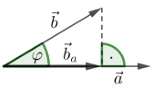
\includegraphics[width=0.9\linewidth]{vec-proj.png}
    \end{minipage}
    \begin{remark}
        Die erste Formel gilt für $0<\varphi\leq\frac{\pi}{2}$,
        die zweite für $\frac{\pi}{2}<\varphi\leq\pi$
    \end{remark}


\paragraph*{Lineare Abhängigkeit und Komponentendarstellung}

\begin{definition}{Linearkombination (LK)}
    $\lambda_1\cdot\vec{a_1}+\lambda_2\cdot\vec{a_2}+\ldots+\lambda_n\cdot\vec{a_n}$
    
    \vspace*{2mm}

    mit $\lambda_n\in R$ heisst \textit{Linearkombination} der Vektoren $\vec{a_1},\ldots,\vec{a_n}$.
\end{definition}

\begin{definition}{Lineare Abhängigkeit}
    $\overrightarrow{a_{1}}, \overrightarrow{a_{2}}, \ldots, \overrightarrow{a_{k}}$ sind linear unabhängig, wenn:
    \vspace*{1mm}
    \begin{itemize}
    \item $\lambda_{1} \cdot \overrightarrow{a_{1}}+\lambda_{2} \cdot \overrightarrow{a_{2}}+\cdots+\lambda_{k} \cdot \overrightarrow{a_{k}} \neq \overrightarrow{0}(\lambda>0 \wedge \lambda \in \mathbb{R})$
    \item $0 \cdot \overrightarrow{a_{1}}+0 \cdot \overrightarrow{a_{2}}+\cdots+0 \cdot \overrightarrow{a_{k}}$ als einzige LK $\overrightarrow{0}$ ergibt
\end{itemize}
\end{definition}

\begin{definition}{Komponentendarstellung} $\vec{a}=a_1\cdot\vec{e}_1+\cdots+a_n\cdot\vec{e}_n=
    \begin{psmallmatrix}
        a_1\\\scalebox{0.5}{\vdots}\\a_n
    \end{psmallmatrix}$

    $\exists a_1, ... a_n \in \R$ (Komponente), so dass
    jeder Vektor $\vec{a}$ \\als LK von $\vec{e}_1,...\vec{e}_n$
    eindeutig dargestellt werden kann. 
\end{definition}

\begin{definition}{Ortsvektor}
    $\vec{r}(P)=\overrightarrow{OP}=x_1\cdot\vec{e}_1+...+x_n\cdot\vec{e}_n =
    \begin{psmallmatrix}
        x_1\\\scalebox{0.5}{\vdots}\\x_n
    \end{psmallmatrix}$
    
    Zu jedem Punkt $P$ des Vektorraums definiert! Ortsvektoren sind im Ursprung $O$ angeheftet, wie jeder Vektor LK 
    von $\vec{e_1}, ... \vec{e_n}$ und lassen sich in Komponentenschreibweise darstellen:
\end{definition}

\begin{minipage}{0.6\linewidth}
\begin{formula}{Komponentendarstellung von $\overrightarrow{OP}$}
    
    $\vec{r}(Q)=\vec{r}(P)+\overrightarrow{PQ}\\
    \Rightarrow \overrightarrow{PQ}=\vec{r}(Q)-\vec{r}(P)=\begin{pmatrix}
        x_Q-x_P\\
        y_Q-y_P\\
        \cdots-\cdots
    \end{pmatrix}$
\end{formula}
\end{minipage}
\begin{minipage}{0.38\linewidth}
    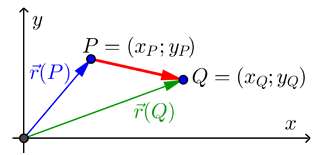
\includegraphics[width=\linewidth]{vec-komp-calc.png}
\end{minipage}


\raggedcolumns


\subsubsection*{Geraden und Ebenen}

\paragraph*{Kollinear und Komplanar}   

\begin{definition}{Kollinear} $\vec{a}$ und $\vec{b}$\\
    \begin{minipage}{0.8\linewidth}
    \begin{itemize}
        \item $\exists$ eine Gerade $g$, zu der beide parallel sind
        \item Spezialfall: Nullvektor ist zu jedem Vektor kollinear
        \item $\vec{a} \times \vec{b} = \vec{0}$ (Kreuzprodukt)
        \item $\vec{a}=\lambda\cdot\vec{b}$ (einer ist Vielfaches des anderen)
    \end{itemize}
    \end{minipage}
    \hspace{3mm}
    \begin{minipage}{0.1\linewidth}
        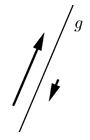
\includegraphics[width=1\linewidth]{vec-kollinear.png}
    \end{minipage}
\end{definition}

\begin{theorem}{Lage} von Geraden im Raum\\
    \vspace*{2mm}
    %make a table to show the different cases
    \begin{tabular}{c|c|c|}
        & Gemeinsame Punkte & keine gem. Punkte \\
        \hline
        Kollinear & Identisch & echt Parallel \\
        \hline
        nicht kollinear & Schneidend & Windschief \\
        \hline
    \end{tabular}
\end{theorem}

\begin{minipage}{0.8\linewidth}
\begin{definition}{Komplanar} $\vec{a}$, $\vec{b}$ und $\vec{c}$\\
    Es existiert eine Ebene $E$, zu der alle parallel sind.
\end{definition}
\end{minipage}
\begin{minipage}{0.15\linewidth}
    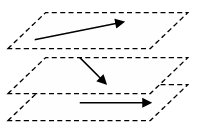
\includegraphics[width=\linewidth]{vec-komplanar.png}
\end{minipage}

\begin{minipage}{0.7\linewidth}
    \begin{theorem}{LK komplanarer Vektoren} $\vec{a}$, $\vec{b}$ und $\vec{c}$\\
        Wenn $\vec{a}$ und $\vec{b}$ nicht kollinear sind lässt sich $\vec{c}$ als Linearkombination von $\vec{a}$ und $\vec{b}$ mit $\lambda, \mu \in \R$ darstellen:
            {\large$\vec{c}=\lambda\cdot\vec{a}+\mu\cdot\vec{b}$}
    \end{theorem}
    \end{minipage}
    \begin{minipage}{0.25\linewidth}
        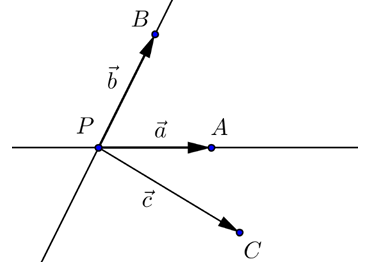
\includegraphics[width=\linewidth]{vec-kompl.png}
\end{minipage}

\begin{minipage}{0.7\linewidth}
    \begin{theorem}{LK nicht komplanarer Vektoren} $\vec{a}$, $\vec{b}$ und $\vec{c}$\\
        Jeder Vektor $\vec{d}$ im $\R^3$ lässt sich als Linearkombination von $\vec{a}$, $\vec{b}$ und $\vec{c}$ eindeutig darstellen:
            {\large$\vec{d}=\lambda\cdot\vec{a}+\mu\cdot\vec{b}+\nu\cdot\vec{c}$}
    \end{theorem}
    \end{minipage}
    \begin{minipage}{0.25\linewidth}
        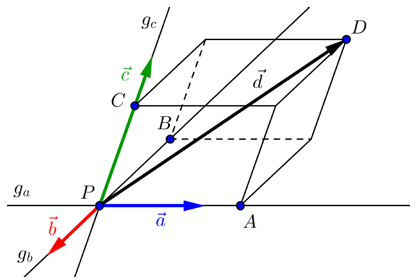
\includegraphics[width=\linewidth]{vec-nicht-kompl.png}
\end{minipage}

\paragraph{Darstellungsformen von Ebenen und Geraden}

\begin{minipage}{0.6\linewidth}
    \begin{definition}{Parameterdarstellung} einer Geraden
        $$\overrightarrow{r}(A) = \overrightarrow{r}(P) + \lambda \cdot \overrightarrow{PQ}$$
    
        {\small Der Punkt $P$ heisst \textit{Aufpunkt}, der Vektor $\overrightarrow{a} = \overrightarrow{PQ}$ heisst \textit{Richtungsvektor} von $g$.}
    \end{definition}
\end{minipage}
\begin{minipage}{0.4\linewidth}
    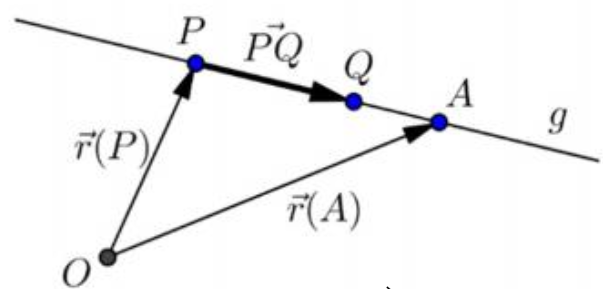
\includegraphics[width=1\linewidth]{gerade.png}\\
    $g: \overrightarrow{r}(P) + \lambda \cdot \overrightarrow{a}$
\end{minipage}


\begin{minipage}{0.6\linewidth}
\begin{definition}{Parameterdarstellung} einer Ebene
    $$E:\,\vec{r}(P)+\lambda\cdot\vec{a}+\mu\cdot\vec{b}\, (\lambda,\mu\in\R)$$
    $P$ = \textit{Aufpunkt}, $a=\overrightarrow{PQ}$ und 
    $\vec{b}=\overrightarrow{PR}$ sind \textit{Richtungsvektoren} von $E$.\\

    Parameterdarstellung nicht eindeutig!\\ Richtungsvektoren zwei beliebige
    Vektoren: \textit{parallel} zu $E$ und \textit{nicht kollinear}
\end{definition}
\end{minipage}
\begin{minipage}{0.4\linewidth}
    \begin{center}
    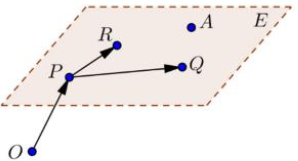
\includegraphics[width=0.8\linewidth]{ebene.png}
    \end{center}
    $\overrightarrow{PA}$, $\overrightarrow{PR}$, $\overrightarrow{PQ}$ komplanar\\

    $\overrightarrow{PA} = \lambda \cdot \overrightarrow{PR} + \mu \cdot \overrightarrow{PQ}$
\end{minipage}


\begin{definition}{Koordinatendarstellung} $a,b,c,d\in \R$
    $$E:\,ax+by+cz+d=0$$
    Bedeutung: die Ebene E besteht aus allen Punkten $P$, deren Koordinaten
    $x, y$ und $z$ diese Gleichung erfüllen.
    $\abs{d}$ = Abstand zum Ursprung, wenn Gleichung normiert
    (sonst $\frac{\vec{d}}{\vec{n}}$)
    {\small
    $$\vec{n} = \begin{pmatrix} a \\ b \\ c \end{pmatrix}, \quad
    \vec{n} \perp \begin{pmatrix} x \\ y \\ z \end{pmatrix}, \quad
    \begin{pmatrix} x \\ y \\ z \end{pmatrix} \cdot \begin{pmatrix} a \\ b \\ c \end{pmatrix} = 0$$
    }
\end{definition}

\paragraph*{Umrechnung von Parameter- und Koordinatendarstellung}

\begin{formula}{Umrechnung Parameterdarstellung zu Koordinatendarstellung}\\
    Berechnen über den Normalenvektor aus dem Kreuzprodukt der Richtungsvektoren,
    welches die Koeffizienten $a, b$ und $c$ liefert. 
    Der Aufpunkt wird über das Einsetzen eines Punktes der Ebene $E$ ermittelt.
    $$
        \vec{n}=\vec{a}\times\vec{b}=\begin{psmallmatrix}
            a\\b\\c
        \end{psmallmatrix}
    $$
\end{formula}

\begin{example2}{Parameterdarstellung $\rightarrow$ Koordinatendarstellung}
    $$E: \begin{psmallmatrix} 2 \\ 4 \\ 1 \end{psmallmatrix} + \lambda \cdot \begin{psmallmatrix} 1 \\ 3 \\ 1 \end{psmallmatrix} + \mu \cdot \begin{psmallmatrix} 2 \\ 2 \\ -4 \end{psmallmatrix}$$
    $$\vec{n} = \begin{psmallmatrix} 1 \\ 3 \\ 1 \end{psmallmatrix} \times \begin{psmallmatrix} 2 \\ 2 \\ -4 \end{psmallmatrix} = \begin{psmallmatrix} -12 -2 \\ 2 + 4 \\ 2 - 6 \end{psmallmatrix} = \begin{psmallmatrix} -14 \\ -6 \\ -4 \end{psmallmatrix}$$
    $$E: -14x - 6y - 4z + d = 0$$
    Aufpunkt einsetzen: $-14 \cdot 2 - 6 \cdot 4 - 4 \cdot 1 + d = 0 \Rightarrow d = 8$
\end{example2}

\begin{formula}{Umrechnung Koordinatendarstellung zu Parameterdarstellung}\\
    Um eine Koordinatendarstellung in eine Parameterdarstellung umzurechnen,
    werden drei Punkte berechnet.
    Einer dieser Punkte wird dann als aufpunkt gewählt und mit den restlichen
    werden Richtungsvektoren berechnet.
\end{formula}

\begin{example2}{Koordinatendarstellung $\rightarrow$ Parameterdarstellung}
    $$E: 2x + 7y - 4z + 1 = 0$$
    Punkte einsetzen: $(0|0|z), (1|0|z), (0|1|z)$\\
    \begin{minipage}{0.5\linewidth}
    \begin{itemize}
        \item $2 \cdot 0 + 7 \cdot 0 - 4 \cdot z + 1 = 0 \Rightarrow z = \frac{1}{4}$
        \item $2 \cdot 1 + 7 \cdot 0 - 4 \cdot z + 1 = 0 \Rightarrow z = \frac{3}{4}$
        \item $2 \cdot 0 + 7 \cdot 1 - 4 \cdot z + 1 = 0 \Rightarrow z = \frac{8}{4}$
    \end{itemize}
    \end{minipage}
    \hspace{2mm}
    \begin{minipage}{0.45\linewidth}
    $E: \begin{psmallmatrix} 0 \\ 0 \\ \frac{1}{4} \end{psmallmatrix} +
    \lambda \begin{psmallmatrix} 1 \\ 0 \\ \frac{2}{4} \end{psmallmatrix} +
    \mu \begin{psmallmatrix} 0 \\ 1 \\ \frac{7}{4} \end{psmallmatrix}$
    \end{minipage}
\end{example2}



\paragraph*{Abstände berechnen}


\begin{formula}{Abstand Punkt-Gerade}Gesucht ist der Fusspunkt $B\in g$\\
    Gegeben: Gerade $g=\vec{r}(P)+\lambda\cdot\vec{a}$ in Parameterform und Punkt $A$
    
    \begin{minipage}{0.59\linewidth}
        \begin{enumerate}
            \item Da $B\in g\Rightarrow \vec{r}(B)=\vec{r}(P)+\lambda_B\cdot\vec{a}$ 
            \item $\vec{BA}=\vec{r}(A)-\vec{r}(B)$
            \item $\vec{BA}\perp g\Rightarrow\vec{BA}\cdot\vec{a}=0$
            \item $l=\abs{\vec{BA}}$ ($\lambda_B$ in $\vec{BA}$ einsetzen)
        \end{enumerate}
    \end{minipage}
    \begin{minipage}{0.4\linewidth}
        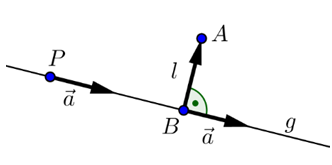
\includegraphics[width=1\linewidth]{vec-abstand-von-punkt.png}
    \end{minipage}

    Meist einfacher:
    $\vec{PA}=\vec{r}(A)-\vec{r}(P) \Rightarrow l=\frac{\abs{\vec{PA}\times\vec{a}}}{\abs{\vec{a}}}$   
\end{formula}

\begin{formula}{Abstand Punkt-Ebene} $l$ = Abstand von $A$ zu $E$\\
    \begin{minipage}{0.7\linewidth}
    Gegeben: Punkt $A=(x_A;y_A;z_A)$, Ebene $E$ mit der \textbf{normierten} 
    Koordinatendarstellung $E:\,ax+by+cz+d=0$
    \begin{center}
    $l=\abs{ax_A+by_A+cz_A+d}$
    \end{center}
    \end{minipage}
    \hspace{3mm}
    \begin{minipage}{0.2\linewidth}
        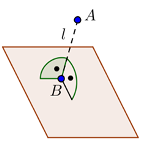
\includegraphics[width=1\linewidth]{vec-abstand-von-ebene.png}
    \end{minipage}

    \begin{minipage}{0.65\linewidth}
        \textbf{nicht normierte} Koordinatendarstellung:
    $$l=\frac{\abs{ax_A+by_A+cz_A+d}}{\abs{\vec{n}}}$$
    \end{minipage}
    \begin{minipage}{0.3\linewidth}
        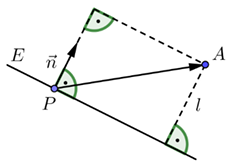
\includegraphics[width=0.9\linewidth]{vec-abstand-von-ebene2.png}
    \end{minipage}
\end{formula}


\section{Geometrische Transformationen}

\subsection{$\R^2$}

\begin{formula}{Streckung}\\
    \begin{minipage}{0.4\linewidth}
        \begin{itemize}
            \item in $x$-Richtung um $\lambda_1$
            \item in $y$-Richtung um $\lambda_2$
        \end{itemize}
    \end{minipage}
    \begin{minipage}{0.6\linewidth}
        $$\begin{pmatrix} x' \\ y' \end{pmatrix} = \begin{pmatrix} \lambda_1 & 0 \\ 0 & \lambda_2 \end{pmatrix} \cdot \begin{pmatrix} x \\ y \end{pmatrix}$$
    \end{minipage}
\end{formula}

\begin{formula}{Spiegelung}\\
    \begin{minipage}{0.45\linewidth}
        \begin{itemize}
            \item Gerade $g: ax + by = 0$
            \item mit $a^2 + b^2 = 1$
        \end{itemize}
    \end{minipage}
    \begin{minipage}{0.5\linewidth}
        $$\begin{pmatrix} 1 - 2a^2 & -2ab \\ -2ab & 1 - 2b^2 \end{pmatrix}$$
    \end{minipage}
\end{formula}

\begin{example}
    \begin{minipage}{0.5\linewidth}
        \begin{itemize}
            \item Gerade $g: x + 7y = 0$
            \item Normiert $g: \frac{1}{\sqrt{50}} x + \frac{7}{\sqrt{50}} y = 0$
        \end{itemize}
    \end{minipage}
    \begin{minipage}{0.45\linewidth}
        $$\frac{1}{50} \cdot \begin{pmatrix} 48 & -14 \\ -14 & -48 \end{pmatrix}$$
    \end{minipage}
\end{example}

\begin{formula}{Orthogonale Projektion}\\
    \begin{minipage}{0.5\linewidth}
    \begin{itemize}
        \item auf Gerade $g: ax + by = 0$
        \item mit $a^2 + b^2 = 1$
    \end{itemize}
    \end{minipage}
    \begin{minipage}{0.5\linewidth}
    $$\begin{pmatrix} 1 - a^2 & -ab \\ -ab & 1-b^2 \end{pmatrix}$$
    \end{minipage}
\end{formula}

\begin{example}
    \begin{minipage}{0.5\linewidth}
    \begin{itemize}
        \item Gerade $g: 2x -y = 0$
        \item Normiert $g: \frac{2}{\sqrt{5}} x - \frac{1}{\sqrt{5}} y = 0$ 
    \end{itemize}
    \end{minipage}
    \begin{minipage}{0.45\linewidth}
    $$\frac{1}{5} \cdot \begin{pmatrix} 1 & 2 \\ 2 & 4 \end{pmatrix}$$
    \end{minipage}
\end{example}

\begin{formula}{Rotation}\\
    \begin{minipage}{0.35\linewidth}
    \begin{itemize}
        \item um den Ursprung
        \item um Winkel $\alpha$
    \end{itemize}
    \end{minipage}
    \begin{minipage}{0.65\linewidth}
    $$\begin{pmatrix} x' \\ y' \end{pmatrix} = \begin{pmatrix} \cos(\alpha) & -\sin(\alpha) \\ \sin(\alpha) & \cos(\alpha) \end{pmatrix} \cdot \begin{pmatrix} x \\ y \end{pmatrix}$$
    \end{minipage}
\end{formula}

\begin{formula}{Scherung}\\
    \begin{minipage}{0.5\linewidth}
    \begin{itemize}
        \item in $x$-Richtung um $s_1$
        \item in $y$-Richtung um $s_2$
    \end{itemize}
    \end{minipage}
    \begin{minipage}{0.5\linewidth}
    $$\begin{pmatrix} x' \\ y' \end{pmatrix} = \begin{pmatrix} 1 & s_1 \\ s_2 & 1 \end{pmatrix} \cdot \begin{pmatrix} x \\ y \end{pmatrix}$$
    \end{minipage}
\end{formula}

\columnbreak

\subsection*{$\R^3$}

\begin{formula}{Zentrische Streckung}\\
    \begin{minipage}{0.4\linewidth}
    \begin{itemize}
        \item in $x$-Richtung um $\lambda_1$
        \item in $y$-Richtung um $\lambda_2$
        \item in $z$-Richtung um $\lambda_3$
    \end{itemize}
    \end{minipage}
    \begin{minipage}{0.5\linewidth}
    $$\begin{pmatrix} x' \\ y' \\ z' \end{pmatrix} = \begin{pmatrix} \lambda_1 & 0 & 0 \\ 0 & \lambda_2 & 0 \\ 0 & 0 & \lambda_3 \end{pmatrix} \cdot \begin{pmatrix} x \\ y \\ z \end{pmatrix}$$
    \end{minipage}
\end{formula}

\begin{formula}{Spiegelung} an der Ebene\\
    \begin{minipage}{0.45\linewidth}
    \begin{itemize}
        \item Ebene $E: ax + by + cz = 0$
        \item mit $a^2 + b^2 + c^2 = 1$
    \end{itemize}
    \end{minipage}
    \begin{minipage}{0.5\linewidth}
    $$\begin{pmatrix} 1 - 2a^2 & -2ab & -2ac \\ -2ab & 1 - 2b^2 & -2bc \\ -2ac & -2bc & 1 - 2c^2 \end{pmatrix}$$
    \end{minipage}
    $$S = E - 2\vec{n} \cdot \vec{n}^T$$
\end{formula}

\begin{example}
    \begin{minipage}{0.5\linewidth}
    \begin{itemize}
        \item Ebene $E: x + 2y + 3z = 0$
        \item Normiert $E: \frac{1}{\sqrt{14}} x + \frac{2}{\sqrt{14}} y + \frac{3}{\sqrt{14}} z = 0$
    \end{itemize}
    \end{minipage}
    \begin{minipage}{0.45\linewidth}
    $$\frac{1}{14} \cdot \begin{pmatrix} 11 & 4 & 6 \\ 4 & 7 & 6 \\ 6 & 6 & 7 \end{pmatrix}$$
    \end{minipage}
\end{example}

\begin{formula}{Orthogonale Projektion} auf die Ebene\\
    \begin{minipage}{0.5\linewidth}
    \begin{itemize}
        \item Ebene $E: ax + by + cz = 0$
        \item mit $a^2 + b^2 + c^2 = 1$
    \end{itemize}
    \end{minipage}
    \begin{minipage}{0.5\linewidth}
    $$\begin{pmatrix} 1 - a^2 & -ab & -ac \\ -ab & 1 - b^2 & -bc \\ -ac & -bc & 1 - c^2 \end{pmatrix}$$
    \end{minipage}
    $$P = E - \vec{n} \cdot \vec{n}^T$$
\end{formula}

\begin{example}
    \begin{minipage}{0.5\linewidth}
    \begin{itemize}
        \item Ebene $E: 2x - y + 3z = 0$
        \item Normiert $E: \frac{2}{\sqrt{14}} x - \frac{1}{\sqrt{14}} y + \frac{3}{\sqrt{14}} z = 0$
    \end{itemize}
    \end{minipage}
    \begin{minipage}{0.45\linewidth}
    $$\frac{1}{14} \cdot \begin{pmatrix} 13 & 4 & 6 \\ 4 & 13 & 9 \\ 6 & 9 & 13 \end{pmatrix}$$
    \end{minipage}
\end{example}

\begin{formula}{Rotation}um den Winkel $\alpha$ um die x, y, z Achsen\\
    \begin{minipage}{0.45\linewidth}
    $$\text{x: } \begin{pmatrix} 1 & 0 & 0 \\ 0 & \cos(\alpha) & -\sin(\alpha) \\ 0 & \sin(\alpha) & \cos(\alpha) \end{pmatrix}$$
    \end{minipage}
    \begin{minipage}{0.45\linewidth}
    $$\text{y: } \begin{pmatrix} \cos(\alpha) & 0 & \sin(\alpha) \\ 0 & 1 & 0 \\ -\sin(\alpha) & 0 & \cos(\alpha) \end{pmatrix}$$
    \end{minipage}
    \\
    $$\text{z: } \begin{pmatrix} \cos(\alpha) & -\sin(\alpha) & 0 \\ \sin(\alpha) & \cos(\alpha) & 0 \\ 0 & 0 & 1 \end{pmatrix}$$
    
\end{formula}


\begin{formula}{Rotation} um den Winkel $\alpha$ um die Gerade g
    
    Gerade $g: \vec{r} = \vec{a} + t \cdot \vec{b}$ mit $|\vec{b}| = 1$

    $\vec{a}$ ist ein Punkt auf der Geraden g, $\vec{b}$ ist der Richtungsvektor der Geraden g

    \vspace{3mm}
   
    $\begin{pmatrix} \cos(\alpha) + a^2(1 - \cos(\alpha)) & ab(1 - \cos(\alpha)) - b \sin(\alpha) & ... \\ 
        ab(1 - \cos(\alpha)) + b \sin(\alpha) & \cos(\alpha) + b^2(1 - \cos(\alpha)) & ... \\ 
        -a \sin(\alpha) + b(1 - \cos(\alpha)) & b \sin(\alpha) + a(1 - \cos(\alpha)) & ... \end{pmatrix}$  
    
    \begin{flushright}
    $\begin{pmatrix} ... & ... & a \sin(\alpha) + b(1 - \cos(\alpha)) \\ 
        ... & ... & -b \sin(\alpha) + a(1 - \cos(\alpha)) \\ 
        ... & ... & \cos(\alpha) + (a^2 + b^2)(1 - \cos(\alpha)) \end{pmatrix}$  
    \end{flushright}

        \vspace{3mm}

        {\small $\uparrow$ 3x3 Matrix, die die Rotation um die Gerade g beschreibt (hat nicht auf eine Zeile gepasst)}
\end{formula}















	\raggedcolumns
	\pagebreak
	
\section*{LGS und Matrizen}

\subsubsection*{Matrizen}

    \begin{definition}{Matrix}
        Tabelle mit $m$ Zeilen und $n$ Spalten: $m \times n$-Matrix $A$\\
        $a_{ij}$: Element in der $i$-ten Zeile und $j$-ten Spalte
    \end{definition}
    
    \begin{minipage}{0.5\linewidth}
    \begin{formula}{Addition und Subtraktion}
        \begin{itemize}
            \item $A + B = C$
            \item $c_{ij} = a_{ij} + b_{ij}$
        \end{itemize}
    \end{formula}
    \end{minipage}
    \begin{minipage}{0.5\linewidth}
    \begin{formula}{Skalarmultiplikation}
        \begin{itemize}
            \item $k \cdot A = B$
            \item $b_{ij} = k \cdot a_{ij}$
        \end{itemize}
    \end{formula}
    \end{minipage}

    \begin{theorem}{Rechenregeln für die Addition und skalare Multiplikation von Matrizen}
        Kommutativ-, Assoziativ- und Distributiv-Gesetz gelten für Matrix-Addition
    \end{theorem}
    
    \begin{formula}{Matrixmultiplikation} $A^{m \times n}$, $B^{n \times k}$\\
        \begin{minipage}{0.6\linewidth}
        Bedingung: $A$ $n$ Spalten, $B$ $n$ Zeilen.\\
        Resultat: $C$ hat $m$ Zeilen und $k$ Spalten.
        \begin{itemize}
            \item $A \cdot B = C$
            \item $c_{ij} = a_{i1} \cdot b_{1j} + a_{i2} \cdot b_{2j} + \ldots + a_{in} \cdot b_{nj}$
            \item $A \cdot B \neq B \cdot A$
        \end{itemize}  
        \end{minipage}
        \begin{minipage}{0.35\linewidth} 
        \begin{center}
        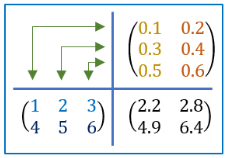
\includegraphics[width=0.8\linewidth]{matrixmultiplikation.png}
        \end{center}
        \end{minipage}
    \end{formula}
    
     \begin{theorem}{Rechenregeln für die Multiplikation von Matrizen}\\
        Assoziativ, Distributiv, nicht Kommutativ!
    \end{theorem}

    \begin{minipage}{0.65\linewidth}
        \begin{definition}{Transponierte Matrix} $A^{m \times n} \rightarrow (A^T)^{n \times m}$
            \begin{itemize}
                \item $A^T$: Spalten und Zeilen vertauscht
                \item $(A^T)_{ij} = A_{ji}$ und ${(A\cdot B)}^T = B^T\cdot A^T$
            \end{itemize}
        \end{definition}
    \end{minipage}
    \begin{minipage}{0.35\linewidth}
        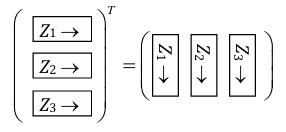
\includegraphics[width=1\linewidth]{mat-transpos.png}
    \end{minipage}

    \begin{KR}{Spezielle Matrizen}
        \begin{itemize}
            \item \textbf{Symmetrische Matrix}: $A^T = A$
            \item \textbf{Einheitsmatrix}: $E$ mit $e_{ij} = 1$ für $i = j$ und $e_{ij} = 0$ für $i \neq j$
            \item \textbf{Diagonalmatrix}: $a_{ij} = 0$ für $i \neq j$
            \item \textbf{Dreiecksmatrix}: $a_{ij} = 0$ für $i > j$ (obere Dreiecksmatrix) \\oder $i < j$ (untere Dreiecksmatrix)
        \end{itemize}
    \end{KR}

\subsubsection*{Lineare Gleichungssysteme (LGS)}
    
        \begin{definition}{Lineares Gleichungssystem (LGS)}
            Ein \textit{lineares Gleichungssystem} ist eine Sammlung von Gleichungen, 
            die linear in den Unbekannten sind. 
            Ein LGS kann in Matrixform $A\cdot\vec{x}=\vec{b}$ dargestellt werden.\\
            \begin{minipage}
                {0.45\linewidth}
                {\small
                $A$: Koeffizientenmatrix\\
                $\vec{x}$: Vektor der Unbekannten\\
                $\vec{b}$: Vektor der Konstanten}
            \end{minipage}
            \begin{minipage}{0.55\linewidth}
                $\begin{psmallmatrix} a_{11} & \cdots & a_{1n} \\ \scalebox{0.5}{\vdots} & \cdots & \scalebox{0.5}{\vdots} \\ a_{m1} & \cdots & a_{mn} \end{psmallmatrix} \cdot \begin{psmallmatrix}
                    x_1 \\ \scalebox{0.5}{\vdots} \\ x_n
                \end{psmallmatrix} = \begin{psmallmatrix}
                    b_1 \\ \scalebox{0.5}{\vdots} \\ b_m
                \end{psmallmatrix}$
            \end{minipage}
        \end{definition}

    
        \begin{theorem}{Rang einer Matrix} $rg(A)$ = Anzahl Zeilen - Anzahl Nullzeilen
            
            $\Rightarrow$ Anzahl linear unabhängiger Zeilen- oder Spaltenvektoren
        \end{theorem}


\begin{concept}{Zeilenstufenform (Gauss)}
    \begin{itemize}
        \item Alle Nullen stehen unterhalb der Diagonalen, Nullzeilen zuunterst
        \item Die erste Zahl $\neq 0$ in jeder Zeile ist eine führende Eins
        \item Führende Einsen, die weiter unten stehen $\rightarrow$ stehen weiter rechts
    \end{itemize}
    \textbf{Reduzierte Zeilenstufenform: (Gauss-Jordan)}\\
    Alle Zahlen links und rechts der führenden Einsen sind Nullen.
\end{concept}

\begin{KR}{Zeilenperationen} erlaubt bei LGS (z.B. Gauss-Verfahren)
        \begin{itemize}
            \item Vertauschen von Zeilen
            \item Multiplikation einer Zeile mit einem Skalar
            \item Addition eines Vielfachen einer Zeile zu einer anderen
        \end{itemize}
    \end{KR}
    
    \begin{formula}{Gauss-Jordan-Verfahren}
        \begin{enumerate}
            \item bestimme linkeste Spalte mit Elementen $\neq 0$ (Pivot-Spalte)
            \item oberste Zahl in Pivot-Spalte $= 0$\\ $\rightarrow$ vertausche Zeilen so dass $a_{11} \neq 0$
            \item teile erste Zeile durch $a_{11}$ $\rightarrow$ so erhalten wir führende Eins
            \item Nullen unterhalb führender Eins erzeugen (Zeilenperationen)
        \end{enumerate}
        nächste Schritte: ohne bereits bearbeitete Zeilen Schritte 1-4 wiederholen, bis Matrix Zeilenstufenform hat
    \end{formula}

    

    \begin{theorem}{Lösbarkeit von linearen Gleichungssystemen}

        \begin{minipage}{0.5\linewidth}
            \begin{itemize}
                \item Lösbar: $rg(A) = rg(A|b)$
                \item genau eine Lösung: $rg(A) = n$
            \end{itemize}
        \end{minipage}
        \begin{minipage}{0.5\linewidth}
            \begin{itemize}
                \item unendlich viele Lösungen:\\ $rg(A) < n$
            \end{itemize}
        \end{minipage}
    \end{theorem}

    \begin{KR}{Parameterdarstellung} bei unendlich vielen Lösungen

        \begin{minipage}{0.74\linewidth}
            Führende Unbekannte: Spalte mit führender Eins\\
            Freie Unbekannte: Spalten ohne führende Eins
        \end{minipage}
        \begin{minipage}{0.25\linewidth}
            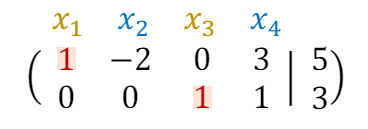
\includegraphics[width=1\linewidth]{parameterdarstellung_lgs.png}
        \end{minipage}

        \vspace{1mm}
        
        Auflösung nach der führenden Unbekannten:
        \begin{itemize}
            \item $1 x_1 - 2 x_2 + 0 x_3 + 3 x_4 = 5 \quad x_2 = \lambda \rightarrow x_1 = 5 + 2 \cdot \lambda - 3 \cdot \mu$
            \item $0 x_1 + 0 x_2 + 1 x_3 + 1 x_4 = 3 \quad x_4 = \mu \rightarrow x_3 = 3 - \mu$    
        \end{itemize}
        \vspace*{2mm}
        $$ \vec{x} = \begin{psmallmatrix} x_1 \\ x_2 \\ x_3 \\ x_4 \end{psmallmatrix} 
        = \begin{psmallmatrix} 5 + 2 \lambda - 3 \mu \\ \lambda \\ 3 - \mu \\ \mu \end{psmallmatrix} 
        = \begin{psmallmatrix} 5 \\ 0 \\ 3 \\ 0 \end{psmallmatrix} + \lambda \begin{psmallmatrix} 2 \\ 1 \\ 0 \\ 0 \end{psmallmatrix} + \mu \begin{psmallmatrix} -3 \\ 0 \\ -1 \\ 1 \end{psmallmatrix}$$
    \end{KR}

    \begin{definition}{Homogenes LGS}
        $\vec{b}=\vec{0} \rightarrow A\cdot\vec{x}=\vec{0} \rightarrow rg(A)=rg(A\mid\vec{b})$\\
        nur zwei Möglichkeiten:
            \begin{itemize}
                \item eine Lösung $x_1=x_2=\cdots=x_n=0$, die sog. \textit{triviale Lösung}.
                \item unendlich viele Lösungen
            \end{itemize}
    \end{definition}

    \begin{theorem}{Koeffizientenmatrix{,} Determinante{,} Lösbarkeit des LGS }\\
        Für $n\times n$-Matrix $A$ sind folgende Aussagen äquivalent:
    
        \vspace{1mm}
    
        \begin{minipage}{0.3\linewidth}
            \begin{itemize}
                \item $\det(A)\neq 0$
                \item $rg(A)=n$
                \item $A$ ist invertierbar
            \end{itemize}
        \end{minipage}
        \begin{minipage}{0.7\linewidth}
            \begin{itemize}
                \item Spalten von $A$ sind linear unabhängig.
                \item Zeilen von $A$ sind linear unabhängig.
                \item LGS $A\cdot\vec{x}=\vec{0}$ \\hat eindeutige Lösung $x=A^{-1}\cdot 0=0$
            \end{itemize}
        \end{minipage}
    \end{theorem}


  

\subsubsection*{Quadratische Matrizen}

\paragraph{Inverse}
    \begin{definition}{Inverse einer quadratischen Matrix A} $A^{-1}$ 
        
        $A^{-1}$ existiert, wenn $rg(A) = n$. $A^{-1}$ ist eindeutig bestimmt.

        \vspace{1mm}

        {\small Eine Matrix heisst \textit{invertierbar / regulär}, wenn sie eine Inverse hat. 
        Andernfalls heisst sie \textit{singulär}}
    \end{definition}
  
    \begin{theorem}{Eigenschaften invertierbarer Matrizen}
        \begin{itemize}
            \item $A\cdot A^{-1}=A^{-1}\cdot A=E$ und $(A^{-1})^{-1}=A$
            \item ${(A\cdot B)}^{-1}=B^{-1}\cdot A^{-1}$ {\small $\quad$ Die Reihenfolge ist relevant!}
            \item $A$ und $B$ invertierbar $\Rightarrow$ $AB$ invertierbar
            \item ${(A^T)^{-1}}={(A^{-1})}^T$ $\quad$ $A$ invertierbar $\Rightarrow$ $A^T$ invertierbar
        \end{itemize}
    \end{theorem}

\begin{theorem}{Inverse einer $2 \times 2$-Matrix} $A = \begin{psmallmatrix} a & b \\ c & d \end{psmallmatrix}$ mit $det(A) = ad - bc$
        $$A^{-1} = \frac{1}{\det(A)} \cdot \begin{pmatrix} d & -b \\ -c & a \end{pmatrix}$$
        NUR Invertierbar falls $ad - bc \neq 0$
\end{theorem}

\begin{KR}{Inverse berechnen} einer quadratischen Matrix $A^{n \times n}$
    $$A \cdot A^{-1} = E \rightarrow \left( A | E \right) \leadsto \text{Zeilenoperationen} \leadsto \left( E | A^{-1}\right)$$
\end{KR}

\begin{concept}{LGS mit Inverse lösen}
    $A \cdot \vec{x} = \vec{b}$
    $$A^{-1} \cdot A \cdot \vec{x} = A^{-1} \cdot \vec{b} \rightarrow \vec{x} = A^{-1} \cdot \vec{b}$$
    Beispiel:\\
    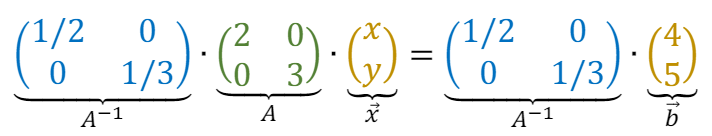
\includegraphics[width=0.7\linewidth]{lgs_inverse.png}
\end{concept}

\subsubsection{Pivotisierung}

\begin{concept}{Permutationsmatrix} $P$ ist eine Matrix, die aus der Einheitsmatrix durch Zeilenvertauschungen entsteht. 
    \vspace{1mm}\\
    \begin{minipage}[t]{0.5\textwidth}
        Für die Vertauschung der $i$-ten und $j$-ten Zeile hat $P_k$ die \textbf{Form}:
        \begin{itemize}
            \item $p_{ii} = p_{jj} = 0$ 
            \item $p_{ij} = p_{ji} = 1$
            \item Sonst gleich wie in $E_n$
        \end{itemize}
    \end{minipage}
    \hspace{3mm}
    \begin{minipage}[t]{0.45\textwidth}
        \vspace{1mm}
        \textbf{Wichtige Eigenschaften}:
        \begin{itemize}
            \item $P^{-1} = P^T = P$
            \item Mehrere Vertauschungen:\\ $P = P_l \cdot ... \cdot P_1$
        \end{itemize}
    \end{minipage}
\end{concept}

\begin{example2}{Zeilenvertauschung} für Matrix A mit Permutationsmatrix $P_1$:
    \vspace{1mm}\\
\begin{minipage}[t]{0.5\textwidth}
    $\underbrace{\begin{psmallmatrix}
    1 & 2 & 3\\
    4 & 5 & 6\\
    7 & 8 & 9
    \end{psmallmatrix}}_{A} \cdot 
    \underbrace{\begin{psmallmatrix}
    0 & 0 & 1\\
    0 & 1 & 0\\
    1 & 0 & 0
    \end{psmallmatrix}}_{P_1} =
    \begin{psmallmatrix}
    7 & 8 & 9\\
    4 & 5 & 6\\
    1 & 2 & 3
    \end{psmallmatrix}$
\end{minipage}
\begin{minipage}[t]{0.45\textwidth}
    \vspace{-2mm}
    $\Rightarrow A \cdot P_1$ bewirkt die Vertauschung von Zeile 1 und 3
\end{minipage}
\end{example2}

\vspace{-1mm}
\subsubsection{Pivotisierung}

\begin{concept}{Spaltenpivotisierung}\\
Strategie zur numerischen Stabilisierung des Gauss-Algorithmus durch Auswahl des betragsmäßig größten Elements als Pivotelement.

Vor jedem Eliminationsschritt in Spalte $i$:
\begin{itemize}
    \item Suche $k$ mit $|a_{ki}| = \max\{|a_{ji}| \mid j = i,\ldots,n\}$
    \item Falls $a_{ki} \neq 0$: Vertausche Zeilen $i$ und $k$
    \item Falls $a_{ki} = 0$: Matrix ist singulär
\end{itemize}
\end{concept}

\begin{KR}{Gauss-Algorithmus mit Pivotisierung}\\
\textbf{1. Elimination (Vorwärts)}:
\begin{itemize}
    \item Für $i=1,\ldots,n-1$:
    \begin{itemize}
    \item Finde $k \geq i$ mit $|a_{ki}| = \max\{|a_{ji}| \mid j = i,\ldots,n\}$
    \item Falls $a_{ki} = 0$: Stop (Matrix singulär)
    \item Vertausche Zeilen $i$ und $k$
    \item Für $j=i+1,\ldots,n$:
    \begin{itemize}
    \item $z_j := z_j - \frac{a_{ji}}{a_{ii}}z_i$
    \end{itemize}
    \end{itemize}
\end{itemize}
\vspace{-2mm}
\resizebox{\columnwidth}{!}{
\textbf{2. Rückwärtseinsetzen}:
$x_i = \frac{b_i - \sum_{j=i+1}^n a_{ij}x_j}{a_{ii}}, \quad i=n,n-1,\ldots,1$
}
\end{KR}

\begin{concept}{Vorteile der Permutationsmatrix}
    \begin{itemize}
        \item Exakte Nachverfolgung aller Zeilenvertauschungen
        \item Einfache Rückführung auf ursprüngliche Reihenfolge durch $P^{-1}$
        \item Kompakte Darstellung mehrerer Vertauschungen
        \item Numerisch stabile Implementierung der Pivotisierung
    \end{itemize}
\end{concept}




	\raggedcolumns
	\columnbreak
	\subsection{Determinante}
    \begin{definition}{Determinante}\\
        Die Determinante gibt an, ob eine Matrix invertierbar ist.
        \begin{equation*}
            \det(A)
            \left\{
                \begin{array}{lll}
                    \neq 0   &\Rightarrow    & A^{-1} \text{ existiert. }\\
                    = 0     &\Rightarrow    & A^{-1} \text{ existiert nicht. }
                \end{array}
            \right.
        \end{equation*}
    \end{definition}

    \begin{theorem}{Eigenschaften von Determinanten}
        Gegeben zweier \textit{quadratischer Matrizen} $A$, $B$ 
        sowie einer \textit{quadratischen Dreiecksmatrix} $D$.
        \begin{align*}
            &\det(E)        &&=1                     \\
            &\det(D)        &&=\prod_{i=1}^n d_{ii}  \\
            &\det(A\cdot B) &&=\det(A)\cdot\det(B)   \\
            &\det(A^T)      &&=\det(A)               \\
            &\det(A^{-1})   &&=\frac{1}{\det(A)}     \\
            &\det(m\cdot A) &&=m^n\cdot\det(A)\, \text{ mit } m\in \R
        \end{align*}
    \end{theorem}

    \begin{theorem}{Geometrische bedeutung der Determinante}


        \begin{wrapfigure}[16]{hr!}{0.35\textwidth}
            \vspace{-10pt}
            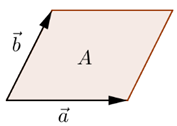
\includegraphics[width=0.9\linewidth]{det-vis-2d.png}
            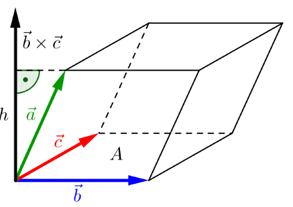
\includegraphics[width=0.9\linewidth]{det-vis-3d.png}
        \end{wrapfigure}
        Die Spalten einer $2\times 2$-Matrix $A$ spannen ein Parallelogram auf.
        Die Determinante der Matrix $A$ ist dabei gerade der \textbf{Flächeninhalt} des aufgespannte Parallelogram.
        \vspace{1.25em}

        Werden Spalten einer $3\times 3$-Matrix $B$ als raum Vektoren betrachtet, 
        spannen diese einen Spat auf.
        Die Determinante der Matrix $A$ ist dabei gerade das $Volumen$ des aufgespannten Spat.
        \vspace{1em}
    \end{theorem}

    \begin{formula}{Determinante einer $1\times 1$-Matrix}
        \begin{equation*}
            \det(A)=A_{11}
        \end{equation*}
    \end{formula}

    \begin{formula}{Determinante einer $2\times 2$-Matrix}
        \begin{equation*}
            \det(A)=\abs{A}=a\cdot d-b\cdot c
        \end{equation*}
    \end{formula}

    \begin{formula}{Determinante einer $3\times 3$-Matrix}\\
        \begin{wrapfigure}{r}{0.4\textwidth}
            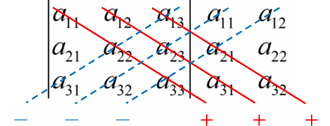
\includegraphics[width=0.9\linewidth]{det3x3.png}
        \end{wrapfigure}
        Die Formel für die Berechnung der Determinante einer $3\times 3$-Matrix ist rechts Gegeben.

        \begin{align*}
            \det(A)&=\abs{A}\\
            &= a_{11}\cdot a_{22}\cdot a_{33} 
            + a_{12}\cdot a_{23}\cdot a_{31} 
            + a_{13}\cdot a_{21}\cdot a_{32}\\
            &- a_{13}\cdot a_{22}\cdot a_{31} 
            - a_{11}\cdot a_{23}\cdot a_{32} 
            - a_{12}\cdot a_{21}\cdot a_{33} 
        \end{align*}
    \end{formula}

    \begin{formula}{Determinante einer $n\times n$-Matrix nach Laplace}\\
        Gegeben einer $n\times n$-Matrix $A$, 
        wird zum berechnen der Determinante eine feste Zeile $i$ oder Spalte $j$ gewählt,
        nachder die Determinante entwickelt wird.

        \textbf{Entwicklung nach Zeile}
        \[\det(A)=\sum_{j=1}^n{(-1)}^{i+j}\cdot A_{ij}\cdot\det(A_{ij})\]
        \textbf{Entwicklung nach Spalte}
        \[\det(A)=\sum_{i=1}^n{(-1)}^{i+j}\cdot A_{ij}\cdot\det(A_{ij})\]

        Bezeichnungen:
        \begin{itemize}
            \item $a_{ij}$ ist das Element der Matrix $A$ in der $i$-ten Zeile und $j$-ten Splate
            \item $A_{ij}$ ist die Matrix, die durch das Weglassen der $i$-ten Zeile und $j$-ten Spalte entsteht. 
        \end{itemize}

        \begin{highlight}{!}
            Um den Rechenaufwand zu minimieren, entwickelt man nach derjenigen Zeile oder Spalte, 
            in der die meisten Nullen stehen. 
        \end{highlight}
    \end{formula}

	\raggedcolumns
	\columnbreak
	

\section{Komplexe Zahlen}

\begin{lemma}{Fundamentalsatz der Algebra}\\
Eine algebraische Gleichung n-ten Grades mit komplexen Koeffizienten:
$$a_nz^n + a_{n-1}z^{n-1} + \cdots + a_1z + a_0 = 0$$
besitzt in $\mathbb{C}$ genau n Lösungen (mit Vielfachheiten gezählt).
\end{lemma}

\begin{concept}{Komplexe Zahlen}\\
Die Menge der komplexen Zahlen $\mathbb{C}$ erweitert die reellen Zahlen $\mathbb{R}$ durch Einführung der imaginären Einheit $i$ mit der Eigenschaft:
$$i^2 = -1$$

Eine komplexe Zahl $z$ ist ein geordnetes Paar $(x,y)$ mit $x,y \in \mathbb{R}$:
$$z = x + iy$$

Die Menge aller komplexen Zahlen ist definiert als:
$$\mathbb{C} = \{z \mid z = x + iy \text{ mit } x,y \in \mathbb{R}\}$$
\end{concept}



\begin{definition}{Bestandteile komplexer Zahlen}\\
\begin{minipage}[t]{0.6\textwidth}
    \vspace{-7mm}
    \textbf{Realteil:} $\operatorname{Re}(z) = x$\\
    \textbf{Imaginärteil:} $\operatorname{Im}(z) = y$\\
    \textbf{Betrag:} $|z| = \sqrt{x^2 + y^2} = \sqrt{z \cdot z^*}$\\
    \textbf{Konjugation:} $\overline{z} = x - iy$
\end{minipage}
\begin{minipage}{0.35\textwidth}
    \vspace{-3mm}
    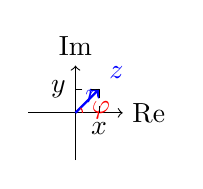
\begin{tikzpicture}[scale=0.3]
        % Coordinate axes
        \draw[->] (-2,0) -- (2,0) node[right] {Re};
        \draw[->] (0,-2) -- (0,2) node[above] {Im};
        
        % Example point and vector
        \draw[thick,blue,->] (0,0) -- (1,1) node[above right] {$z$};
        
        % Angle and labels
        \draw[red] (0.3,0) arc (0:45:0.3) node[midway,right] {$\varphi$};
        
        % Components
        \draw[dashed] (1,1) -- (1,0) node[below] {$x$};
        \draw[dashed] (1,1) -- (0,1) node[left] {$y$};
        
        % Radius
        \node[blue] at (0.7,0.7) {$r$};
    \end{tikzpicture}
\end{minipage}
\end{definition}


\begin{concept}{Darstellungsformen}
\begin{itemize}
    \item Normalform: $z = x + iy$
    \item Trigonometrische Form: $z = r(\cos\varphi + i\sin\varphi)$
    \item Exponentialform: $z = re^{i\varphi}$
\end{itemize}
\end{concept}

\begin{KR}{Umrechnung zwischen Darstellungsformen komplexer Zahlen}
\paragraph{Von Normalform in trigonometrische Form/Exponentialform}
\begin{enumerate}
   \item Berechne Betrag $r = \sqrt{x^2 + y^2}$
   \item Berechne Winkel mit einer der Formeln: 
   \begin{itemize}
       \item $\varphi = \arctan(\frac{y}{x})$ falls $x > 0$
       \item $\varphi = \arctan(\frac{y}{x}) + \pi$ falls $x < 0$
       \item $\varphi = \frac{\pi}{2}$ falls $x = 0, y > 0$
       \item $\varphi = -\frac{\pi}{2}$ falls $x = 0, y < 0$
       \item $\varphi$ unbestimmt falls $x = y = 0$
   \end{itemize}
   \item Trigonometrische Form: $z = r(\cos\varphi + i\sin\varphi)$
   \item Exponentialform: $z = re^{i\varphi}$
\end{enumerate}

\paragraph{Von trigonometrischer Form in Normalform}
\begin{enumerate}
   \item Realteil: $x = r\cos\varphi$
   \item Imaginärteil: $y = r\sin\varphi$
   \item Normalform: $z = x + iy$
\end{enumerate}

\paragraph{Von Exponentialform in Normalform/trigonometrische Form}
\begin{enumerate}
   \item Trigonometrische Form durch Euler-Formel:\\
   $re^{i\varphi} = r(\cos\varphi + i\sin\varphi)$
   \item Dann wie oben in Normalform umrechnen
\end{enumerate}

\paragraph{Wichtige Hinweise:}
\begin{itemize}
   \item Achten Sie auf das korrekte Quadranten beim Winkel
   \item Winkelfunktionen im Bogenmaß verwenden
   \item Bei Umrechnung in Normalform Euler-Formel nutzen
   \item Vorzeichen bei Exponentialform beachten
\end{itemize}
\end{KR}




\begin{theorem}{Rechenoperationen mit komplexen Zahlen}\\
Für $z_1 = x_1 + iy_1$ und $z_2 = x_2 + iy_2$ gilt:
\vspace{1mm}\\
\begin{minipage}[t]{0.45\textwidth}
    \textbf{Addition:}\\
    $z_1 + z_2 = (x_1 + x_2) + i(y_1 + y_2)$
\end{minipage}
\hspace{3mm}
\begin{minipage}[t]{0.45\textwidth}
    \textbf{Subtraktion:}\\
    $z_1 - z_2 = (x_1 - x_2) + i(y_1 - y_2)$
\end{minipage}

\begin{minipage}{0.28\textwidth}
    \textbf{Multiplikation:}
\end{minipage}
\begin{minipage}{0.68\textwidth}
    \begin{align*}
        z_1 \cdot z_2 &= (x_1x_2 - y_1y_2) + i(x_1y_2 + x_2y_1)\\
        &= r_1r_2e^{i(\varphi_1 + \varphi_2)} \text{ (in Exponentialform)}
    \end{align*}
\end{minipage}



\textbf{Division:}
\begin{align*}
    \frac{z_1}{z_2} &= \frac{z_1 \cdot z_2^*}{z_2 \cdot z_2^*} = \frac{(x_1x_2 + y_1y_2) + i(y_1x_2 - x_1y_2)}{x_2^2 + y_2^2}\\
    &= \frac{r_1}{r_2}e^{i(\varphi_1 - \varphi_2)} \text{ (in Exponentialform)}
\end{align*}
\end{theorem}

\begin{corollary}{Potenzen und Wurzeln}\\
Für eine komplexe Zahl in Exponentialform $z = re^{i\varphi}$ gilt:
\begin{itemize}
    \item n-te Potenz: $z^n = r^ne^{in\varphi} = r^n(\cos(n\varphi) + i\sin(n\varphi))$
    \item n-te Wurzel: $z_k = \sqrt[n]{r}e^{i\frac{\varphi + 2\pi k}{n}}$, $k = 0,1,\ldots,n-1$
\end{itemize}
\end{corollary}

\begin{example2}{Komplexe Operationen}
Gegeben $z_1 = 1+i$ und $z_2 = 2-i$:

\paragraph{Umrechnung in Polarform:}
\begin{itemize}
    \item $z_1: r_1 = \sqrt{2}$, $\varphi_1 = \frac{\pi}{4}$
    \item $z_2: r_2 = \sqrt{5}$, $\varphi_2 = -\arctan(\frac{1}{2})$
\end{itemize}

\paragraph{Berechnungen:}
\begin{itemize}
    \item $z_1 \cdot z_2 = (2-i)(1+i) = (2+1) + i(2-1) = 3+i$
    \item $z_1^3 = (\sqrt{2})^3(\cos(\frac{3\pi}{4}) + i\sin(\frac{3\pi}{4}))$
\end{itemize}
\end{example2}

\raggedcolumns
\columnbreak

\section{Eigenwerte und Eigenvektoren}

\begin{definition}{Eigenwerte und Eigenvektoren}\\
Für eine Matrix $A \in \mathbb{R}^{n\times n}$ heißt $\lambda \in \mathbb{C}$ Eigenwert von $A$, wenn es einen Vektor $x \in \mathbb{C}^n \backslash \{0\}$ gibt mit:
\vspace{-2mm}\\
$$Ax = \lambda x$$
Der Vektor $x$ heißt dann Eigenvektor zum Eigenwert $\lambda$.
\end{definition}

\begin{concept}{Bestimmung von Eigenwerten}\\
Ein Skalar $\lambda$ ist genau dann Eigenwert von $A$, wenn gilt:
\vspace{-2mm}\\
$$\det(A - \lambda I_n) = 0 \text{(charakteristische Gleichung)}$$
$$\text{charakteristisches Polynom von }A : p(\lambda) = \det(A - \lambda I_n)$$
\end{concept}

\begin{theorem}{Eigenschaften von Eigenwerten}
Für eine Matrix $A \in \mathbb{R}^{n\times n}$ gilt:

\begin{minipage}{0.5\textwidth}
    $$\text{Determinante: } \det(A) = \prod_{i=1}^n \lambda_i $$
\end{minipage}
\begin{minipage}{0.5\textwidth}
    $$\text{Spur: }\operatorname{tr}(A) = \sum_{i=1}^n \lambda_i$$
\end{minipage}

\begin{itemize}
    \item Bei Dreiecksmatrix sind die Diagonalelemente die Eigenwerte
    \item Ist $\lambda$ Eigenwert von $A$, so ist $\frac{1}{\lambda}$ Eigenwert von $A^{-1}$
\end{itemize}
\end{theorem}

\begin{formula}{Vielfachheiten}
Für einen Eigenwert $\lambda$ unterscheidet man:
\begin{itemize}
    \item Algebraische Vielfachheit: \\Vielfachheit als Nullstelle des charakteristischen Polynoms
    \item Geometrische Vielfachheit: \\Dimension des Eigenraums $= n - \operatorname{rg}(A-\lambda I_n)$
\end{itemize}
Die geometrische Vielfachheit ist stets kleiner oder gleich der algebraischen Vielfachheit.
\end{formula}

\begin{definition}{Diagonalisierbarkeit}
Eine Matrix $A$ ist genau dann diagonalisierbar, wenn sie $n$ linear unabhängige Eigenvektoren besitzt. Dies ist äquivalent zu:
\begin{itemize}
    \item Die algebraischen Vielfachheiten der Eigenwerte entsprechen den geometrischen Vielfachheiten
    \item Die Summe der geometrischen Vielfachheiten ist $n$
    \item Die Matrix $A$ ist ähnlich zu einer Diagonalmatrix
    \item Die Matrix $A$ hat $n$ linear unabhängige Eigenvektoren
\end{itemize}
\end{definition}

\begin{concept}{Ähnliche Matrizen}\\
Zwei Matrizen $A,B \in \mathbb{R}^{n\times n}$ heißen ähnlich, wenn es eine reguläre Matrix $T$ gibt mit:
$$B = T^{-1}AT$$

Eine Matrix $A$ heißt diagonalisierbar, wenn sie ähnlich zu einer Diagonalmatrix $D$ ist:
$$D = T^{-1}AT$$
\end{concept}

\begin{theorem}{Eigenschaften ähnlicher Matrizen}\\
Für ähnliche Matrizen $A$ und $B = T^{-1}AT$ gilt:
\begin{enumerate}
    \item $A$ und $B$ haben dieselben Eigenwerte mit gleichen algebraischen Vielfachheiten
    \item Ist $x$ Eigenvektor von $B$ zum Eigenwert $\lambda$, so ist $Tx$ Eigenvektor von $A$ zum Eigenwert $\lambda$
    \item Bei Diagonalisierbarkeit:
    \begin{itemize}
        \item Die Diagonalelemente von $D$ sind die Eigenwerte von $A$
        \item Die Spalten von $T$ sind die Eigenvektoren von $A$
    \end{itemize}
\end{enumerate}
\end{theorem}

\begin{KR}{Bestimmung von Eigenwerten}

\paragraph{Charakteristisches Polynom aufstellen}
\begin{itemize}
    \item $p(\lambda) = \det(A-\lambda I)$ berechnen und auf Standardform bringen
    \item  Spezialfälle:
    \begin{itemize}
        \item Bei $2 \times 2$ Matrizen direkt: $\det(A - \lambda I)$
        \item Bei $3 \times 3$ Matrizen: Entwicklung nach einer Zeile/Spalte
        \item Bei größeren Matrizen: Spezielle Eigenschaften nutzen
              (z.B. Dreiecksform, Symmetrie)
    \end{itemize}
\end{itemize}
    
    \paragraph{Polynom vereinfachen und auf Nullform bringen}
    \begin{itemize}
        \item Ausmultiplizieren
        \item Zusammenfassen nach Potenzen von $\lambda$
        \item Form: $p(\lambda) = (-1)^n\lambda^n + a_{n-1}\lambda^{n-1} + \cdots + a_1\lambda + a_0$
    \end{itemize}

    \paragraph{Nullstellen bestimmen}
    \begin{itemize}
        \item Quadratische Formel für $n=2$ (Grad des Polynoms)
        \item Cardano-Formel oder Substitution für $n=3$
        \item Numerische Verfahren für $n>3$
    \end{itemize}

    \paragraph{Vielfachheiten bestimmen}
    \begin{itemize}
        \item Algebraische Vielfachheit: Nullstellenordnung
        \item Geometrische Vielfachheit: $n-\operatorname{rang}(A-\lambda I)$
    \end{itemize}
\end{KR}

\begin{example2}{Charakteristisches Polynom}\\
Bestimmen Sie die Eigenwerte von:
$A = \begin{psmallmatrix}
2 & -1 & 0 \\
-1 & 2 & -1 \\
0 & -1 & 2
\end{psmallmatrix}$

\paragraph{Lösung:}
\begin{enumerate}
    \item $p(\lambda) = \det(A-\lambda I)$:
    $\begin{vsmallmatrix}
    2-\lambda & -1 & 0 \\
    -1 & 2-\lambda & -1 \\
    0 & -1 & 2-\lambda
    \end{vsmallmatrix}$
    \vspace{1mm}\\
    \item Determinante:
    $p(\lambda) = (2-\lambda)^3 - 2(2-\lambda) = -\lambda^3 + 6\lambda^2 - 11\lambda + 6$
    \vspace{1mm}\\
    \item Nullstellen:
    $\lambda_1 = 1, \lambda_2 = 2, \lambda_3 = 3$
\end{enumerate}
\end{example2}

\begin{KR}{Bestimmung von Eigenvektoren}

\paragraph{Eigenvektoren bestimmen}
\begin{enumerate}
    \item Für jeden Eigenwert $\lambda_i$:
    \begin{itemize}
        \item Matrix $(A - \lambda_i I)$ aufstellen
        \item Homogenes LGS $(A - \lambda_i I)x = 0$ lösen
        \item Lösungsvektor normieren falls gewünscht
    \end{itemize}

    \item Bei mehrfachen Eigenwerten:
    \begin{itemize}
        \item Geometrische Vielfachheit bestimmen
        \item Basis des Eigenraums bestimmen
        \item Linear unabhängige Eigenvektoren finden
    \end{itemize}
\end{enumerate}

\paragraph{Kontrolle}
\begin{itemize}
    \item Für jeden Eigenvektor $x_i$ prüfen: $Ax_i = \lambda_i x_i$
    \item Bei symmetrischen Matrizen: Orthogonalität der Eigenvektoren prüfen
    \item Linear unabhängigkeit der Eigenvektoren überprüfen
    \item Bei $2 \times 2$ Matrix: $\lambda_1 + \lambda_2 = \operatorname{tr}(A)$ und $\lambda_1 \cdot \lambda_2 = \det(A)$
    \item Bei $3 \times 3$ Matrix zusätzlich: $\sum \lambda_i = \operatorname{tr}(A)$ und $\prod \lambda_i = \det(A)$
    \item Bei reellen Matrizen: Komplexe Eigenwerte treten in konjugierten Paaren auf
\end{itemize}

\paragraph{Spezialfälle beachten}
\begin{itemize}
    \item Bei Dreiecksmatrizen: Eigenwerte sind die Diagonalelemente
    \item Bei symmetrischen Matrizen: Alle Eigenwerte sind reell
    \item Bei orthogonalen Matrizen: $|\lambda_i| = 1$ für alle Eigenwerte
    \item Bei nilpotenten Matrizen: Alle Eigenwerte sind 0\\
    nilpotente Matrix: $A^k = 0$ für ein $k \in \mathbb{N}$
\end{itemize}
\end{KR}

\begin{example2}{Eigenwertberechnung}
Gegeben ist die Matrix
$A = \begin{psmallmatrix} 
2 & 1 & 0 \\
1 & 2 & 1 \\
0 & 1 & 2
\end{psmallmatrix}$

1. Charakteristisches Polynom aufstellen:
   $$\det(A - \lambda I) = \begin{vsmallmatrix} 
   2-\lambda & 1 & 0 \\
   1 & 2-\lambda & 1 \\
   0 & 1 & 2-\lambda
   \end{vsmallmatrix}$$
   
2. Entwicklung nach 1. Zeile:
   $$p(\lambda) = (2-\lambda)\begin{vsmallmatrix}
   2-\lambda & 1 \\
   1 & 2-\lambda
   \end{vsmallmatrix} - 1\begin{vsmallmatrix}
   1 & 1 \\
   1 & 2-\lambda
   \end{vsmallmatrix}$$
   
3. Ausrechnen:
   $$p(\lambda) = (2-\lambda)((2-\lambda)^2 - 1) - ((2-\lambda) - 1)
   = -\lambda^3 + 6\lambda^2 - 11\lambda + 6$$
   
4. Nullstellen bestimmen:
   $\lambda_1 = 1, \lambda_2 = 2, \lambda_3 = 3$
\vspace{1mm}\\
5. Eigenvektoren bestimmen für $\lambda_1 = 1$:
   $$(A - I)x = 0 \text{ führt zu } x_1 = \begin{psmallmatrix} 1 \\ -2 \\ 1 \end{psmallmatrix}$$
\end{example2}

\begin{example2}{Eigenvektoren}
Bestimmen Sie die Eigenvektoren zum Eigenwert $\lambda=2$ der Matrix:
$$A = \begin{psmallmatrix}
2 & 1 & 0 \\
0 & 2 & 0 \\
0 & -1 & 2
\end{psmallmatrix}$$

\paragraph{Lösung:}
\begin{enumerate}
    \item $(A-2I)x = 0$:
    $$\begin{psmallmatrix}
    0 & 1 & 0 \\
    0 & 0 & 0 \\
    0 & -1 & 0
    \end{psmallmatrix} \begin{psmallmatrix}
    x_1 \\ x_2 \\ x_3
    \end{psmallmatrix} = \begin{psmallmatrix}
    0 \\ 0 \\ 0
    \end{psmallmatrix}$$
    
    \item Homogenes System lösen:
    \begin{itemize}
        \item $x_2 = 0$ (aus 1. Zeile)
        \item $x_1, x_3$ frei wählbar
    \end{itemize}
    
    \item Basis des Eigenraums:
    $$v_1 = \begin{psmallmatrix} 1 \\ 0 \\ 0 \end{psmallmatrix}, 
    v_2 = \begin{psmallmatrix} 0 \\ 0 \\ 1 \end{psmallmatrix}$$
\end{enumerate}
\end{example2}



\begin{example2}{Eigenwerte und Eigenvektoren}
Bestimmen Sie Eigenwerte und -vektoren von:
$$A = \begin{psmallmatrix}
2 & -1 \\
-1 & 2
\end{psmallmatrix}$$

\paragraph{Lösung:}
\begin{enumerate}
    \item Charakteristisches Polynom:
    $$\det(A-\lambda I) = \begin{vmatrix} 
    2-\lambda & -1 \\
    -1 & 2-\lambda
    \end{vmatrix} = (2-\lambda)^2 - 1 = 0$$
    
    \item Eigenwerte: $\lambda_1 = 3$, $\lambda_2 = 1$
    
    \item Eigenvektoren für $\lambda_1 = 3$:
    $$(A-3I)x = \begin{psmallmatrix}
    -1 & -1 \\
    -1 & -1
    \end{psmallmatrix}x = 0 \Rightarrow x_1 = \begin{psmallmatrix}
    1 \\
    1
    \end{psmallmatrix}$$
    
    \item Eigenvektoren für $\lambda_2 = 1$:
    $$(A-I)x = \begin{psmallmatrix}
    1 & -1 \\
    -1 & 1
    \end{psmallmatrix}x = 0 \Rightarrow x_2 = \begin{psmallmatrix}
    1 \\
    -1
    \end{psmallmatrix}$$
\end{enumerate}
\end{example2}







	\raggedcolumns
	\pagebreak
	\input{vektorräume.tex}
	\raggedcolumns
	\pagebreak
	

\section{Lineare Abbildungen}


\begin{definition}{Lineare Abbildung} $f: V \rightarrow W$ wo $V$, $W$ reelle Vektorräume\\
    Eine Abbildung $f$ heisst linear, wenn $\forall \overrightarrow{a}, \overrightarrow{b} \in V$, $\forall \lambda \in \mathbb{R}$ gilt:
    $$
    f(\overrightarrow{a} + \overrightarrow{b}) = f(\overrightarrow{a}) + f(\overrightarrow{b})
    \text{ und }
    f(\lambda \cdot \overrightarrow{a} \cdot \vec{b}) = \lambda \cdot f(\overrightarrow{a}) \cdot f(\vec{b})
    $$
    Erlaubte Operationen:\\
    \begin{minipage}{0.6\linewidth}
        \begin{itemize}
            \item Multiplikation mit Skalar: $\lambda \cdot \vec{a}$
        \end{itemize}
    \end{minipage}
    \begin{minipage}{0.3\linewidth}
        \begin{itemize}
            \item Addition: $\vec{a} + \vec{b}$
        \end{itemize}
    \end{minipage}
    
    \vspace{1mm}

    Verbotene Operationen:\\
    \begin{minipage}{0.6\linewidth}
        \begin{itemize}
            \item Multiplikation von Vektoren: $\vec{a} \cdot \vec{b}$
            \item Addition von Skalaren: $\lambda + \vec{a}$
        \end{itemize}
    \end{minipage}
    \begin{minipage}{0.3\linewidth}
        \begin{itemize}
            \item Potenzieren: $\vec{a}^2$
            \item Cosinus: $\cos(\vec{a})$
        \end{itemize}
    \end{minipage}
\end{definition}

\begin{KR}{Überprüfung der Linearität}
    $f: V \rightarrow W$, $f(\vec{x}) \rightarrow \vec{y}$
    \begin{itemize}
        \item $f(\vec{0}) = \vec{0}$
        \item $f(\lambda \cdot \overrightarrow{x_1} \cdot \vec{x_2}) = \lambda \cdot f(\overrightarrow{a}) \cdot f(\vec{b})$
        \item $f(\vec{x_1} + \vec{x_2}) = f(\vec{x_1}) + f(\vec{x_2})$
    \end{itemize}

    \vspace{1mm}

    $\Rightarrow$ Funktionsgleichung einsetzen und überprüfen
\end{KR}

\begin{example}
    $f: \mathbb{R} \rightarrow \mathbb{R}: f(x)=\binom{x_{1}}{x_{2}} \rightarrow\binom{x_{1}+2 x_{2}}{x_{2}}$
    $$
    f\binom{x_{1}+y_{1}}{x_{2}+y_{2}}=\binom{x_{1}+y_{1}+2 \cdot\left(x_{2}+y_{2}\right)}{x_{2}+y_{2}}
    =f\binom{x_{1}}{x_{2}}+f\binom{y_{1}}{y_{2}} \Rightarrow \surd 
    $$
    ... usw.
\end{example}


\begin{definition}{Bild im(A)}
    einer $m \times n$-Matrix $A$, ist der Unterraum des m-dimensionalen Vektorraum $W$, der von den Spalten $\overrightarrow{a_{1}}, \overrightarrow{a_{2}}, \ldots, \overrightarrow{a_{n}}$ der Matrix aufgespannt wird:
    $$
    \operatorname{im}(A)=\operatorname{span}\left(\overrightarrow{a_{1}}, \ldots, \overrightarrow{a_{n}}\right)=\left\{\lambda_{1} \overrightarrow{a_{1}}+\cdots+\lambda_{n} \overrightarrow{a_{n}} \mid \lambda_{1} \in \mathbb{R}\right\}
    $$
\end{definition}

\begin{definition}{Kern ker(A)}
    einer $m \times n$-Matrix $A$ ist die Lösungsmenge des homogenen LGS $A \cdot \vec{x}=\overrightarrow{0}$. Der Kern $\operatorname{ker}(A)$ ist der folgende Unterraum von $V$
    $$\operatorname{ker}(A)=\{\vec{x} \in V \mid A \cdot \vec{x}=\overrightarrow{0}\}$$
\end{definition}



\begin{KR}{Basis für Bild und Kern}
    1. Bringe $A$ in Zeilenstufenform (ZSF)

    \vspace{1mm}

    \begin{minipage}{0.45\linewidth}
        \textcolor{pink}{Bild:}\\
        2. Pivotspalten in der ZSF?\\
        3. Pivotspalten von $A$ (nicht ZSF!) ergeben eine Basis für den Kern
    \end{minipage}
    \hspace{3mm}
    \begin{minipage}{0.5\linewidth}
        \textcolor{pink}{Kern:}\\
        2. LGS $A \cdot \vec{x} = \overrightarrow{0}$ aufstellen\\
        3. Lösungsmenge als LK von Vektoren mit freien Variablen als Koeffizienten ergibt Basis für Kern
    \end{minipage}
\end{KR}



\begin{example}
    \resizebox{\linewidth}{!}{
    $ A = \begin{pmatrix} -1 & 0 & 2 \\ 1 & 6 & 4 \\ 3 & 3 & -3 \end{pmatrix} 
    \Rightarrow \left(\begin{array}{ccc|c}
        -1 & 0 & 2 & 0 \\
        1 & 6 & 4 & 0 \\
        3 & 3 & -3 & 0
        \end{array}\right)=\left(\begin{array}{ccc|c}
        1 & 0 & -2 & 0 \\
        0 & 1 & 1 & 0 \\
        0 & 0 & 0 & 0
        \end{array}\right)
    $}

    \vspace{1mm}

    $$
    x_{1}=2 \lambda, x_{2}=-\lambda, x_{3}=\lambda
    $$

    \vspace{2mm}

    \resizebox{\linewidth}{!}{
    $
    im(A) = \left\{\begin{psmallmatrix} -1 \\ 1 \\ 3 \end{psmallmatrix} \cdot \mu + \begin{psmallmatrix} 0 \\ 6 \\ 3 \end{psmallmatrix} \cdot v \mid \mu, v \in \mathbb{R}\right\}
    \quad
    ker(A) = \left\{\begin{psmallmatrix} 2 \\ -1 \\ 1 \end{psmallmatrix} \cdot \lambda \mid \lambda \in \mathbb{R}\right\}
    $}
\end{example}



\begin{formula}{Zauberzahlen m{,} n{,} r{,}} Für $A^{m \times n}$ mit $rg{A} = r$ gilt:
    $$
    \dim(im(A))=\dim(im(A^{-1}))=r
    $$
    $$
    \dim(ker(A))=n-r
    \text{ und } \dim(ker(A^{-1}))=m-r
    $$
\end{formula}

\subsubsection*{Abbildungsmatrix}

\begin{definition}{Homogene Koordinaten}
    Homogene Koordinaten sind eine Erweiterung des euklidischen Raumes, die es ermöglicht, Punkte im Unendlichen zu repräsentieren.
    Ein Punkt im $\mathbb{R}^2$ wird durch einen Vektor $(x, y, z)$ dargestellt, wobei $z\neq 0$.
    Die Punkte $(x, y, z)$ und $(\lambda x, \lambda y, \lambda z)$ repräsentieren den gleichen Punkt im euklidischen Raum.
    
    {\small nützlich, um Transformationen wie Translationen und Projektionen zu vereinfachen}
\end{definition}

\begin{definition}{Abbildungsmatrix STandardbasis}
    Vektorräume $\mathbb{R}^{m}$ und $\mathbb{R}^{n}$, mit der jeweiligen Standardbasis. Dann lässt sich jede lineare Abbildung $f: \mathbb{R}^{n} \rightarrow \mathbb{R}^{m}$ durch eine $m \times n$ - Matrix $A$ darstellen

    $$
    f(\vec{x})=A \cdot \vec{x}
    $$

    Die Spalten der Matrix $A$ sind die Bilder der Standardbasisvektoren von $\mathbb{R}^{n}$ :

    \begin{center}
    \resizebox{0.7\linewidth}{!}{
    $
    A = \left(f(\overrightarrow{e_{1}}) \scalebox{0.5}{\ldots} f(\overrightarrow{e_{n}})\right)
    = \left(f\begin{psmallmatrix} 1 \\ 0 \\ \scalebox{0.5}{\vdots} \\ 0 \end{psmallmatrix} f\begin{psmallmatrix} 0 \\ 1 \\ \scalebox{0.5}{\vdots} \\ 0 \end{psmallmatrix} \scalebox{0.5}{\ldots} f\begin{psmallmatrix} 0 \\ 0 \\ \scalebox{0.5}{\vdots} \\ 1 \end{psmallmatrix}\right)
    $}
    \end{center}
\end{definition}

\begin{example}
    $$
    f: \mathbb{R}^{2} \rightarrow \mathbb{R}^{3}:\binom{x_{1}}{x_{2}} \rightarrow \begin{psmallmatrix} x_{1}-x_{2} \\ 3 x_{2} \\ -4 x_{1} \end{psmallmatrix}
    \Rightarrow A = \begin{psmallmatrix} 1 & -1 \\ 0 & 3 \\ -4 & 0 \end{psmallmatrix}
    $$
\end{example}

\begin{formula}{Abbildungsmatrix beliebiger Basis}\\
    Wir betrachten zwei endliche Vektorräume
    $$
    V \text { mit Basis } B=\left\{\overrightarrow{b_{1}} ; \ldots ; \overrightarrow{b_{n}}\right\}, W \text { mit Basis } C=\left\{\overrightarrow{c_{1}} ; \ldots ; \overrightarrow{c_{n}}\right\}
    $$

    Jede lineare Abbildung $f: V \rightarrow W$ lässt sich durch eine $m \times n$ - Matrix ${ }_{C} A_{B}$ darstellen

    $$
    (f(\vec{x}))_{C}={ }_{C} A_{B} \cdot \vec{x}_{B}
    $$

    Die Spalten der Matrix ${ }_{C} A_{B}$ sind die Bilder der Elemente von $B$ in der Komponentendarstellung bezüglich der Basis $C$ :
    \begin{center}
    \resizebox{0.8\linewidth}{!}{
    $
    { }_{C} A_{B}={ }_{C}\left(\left(f\left(\overrightarrow{b_{1}}\right)\right)_{C}\left(f\left(\overrightarrow{b_{2}}\right)\right)_{C} \quad \cdots \quad\left(f\left(\overrightarrow{b_{n}}\right)\right)_{C}\right)_{B}
    $
    }
    \end{center}
\end{formula}

\begin{example}
    $$
    f: \mathbb{R}^{2} \rightarrow \mathbb{R}^{3}:\binom{x_{1}}{x_{2}} \rightarrow\begin{psmallmatrix} x_{1}-x_{2} \\ 3 x_{2} \\ -4 x_{1} \end{psmallmatrix}
    $$

    $$
    B=\left\{\binom{1}{0} ; \binom{0}{1}\right\}, C=\left\{\binom{1}{0} ; \binom{1}{1} ; \binom{1}{2}\right\}
    \Rightarrow { }_{C} A_{B}=\begin{psmallmatrix} 1 & -1 \\ 0 & 3 \\ -4 & 0 \end{psmallmatrix}
    $$
\end{example}



\begin{theorem}{Verknüpfungen}
    Wir betrachten zwei lineare Abbildungen
    \begin{itemize}
    \item $f: U \rightarrow V$ mit Abbildungsmatrix $A$
    \item $g: V \rightarrow W$ mit Abbildungsmatrix $B$
    \end{itemize}
    \begin{center}
    %\includegraphics[width=0.4\linewidth]{verknüpfungen.png}\\
    \end{center}
    Die Abbildungsmatrix der Verknüpfung $g \circ f$ ist wieder eine lineare Abbildung mit der Abbildungsmatrix $B \cdot A$.
\end{theorem}

\begin{concept}{Koordinatentransformation}\\
    Die Abbildungsmatrix ${ }_{B} T_{S}$ für den Basiswechsel von $S$ nach $B$
    \begin{itemize}
    \item Die Matrix ${ }_{B} T_{S}$ ist die Inverse von ${ }_{S} T_{B}:{ }_{B} T_{S}=\left({ }_{S} T_{B}\right)^{-1}$
    \end{itemize}
    \begin{center}
    %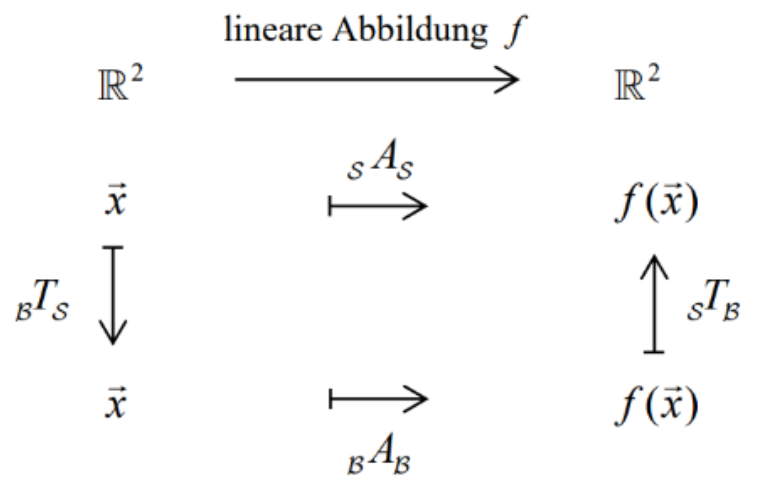
\includegraphics[width=0.6\linewidth]{koordinatentrans.png}
    \end{center}
\end{concept}

\begin{KR}{Basiswechsel mit Koordinatentransformation}\\
    \begin{minipage}{0.45\linewidth}
        \textcolor{pink}{Von Basis $B$ nach Basis $C$}
        $$
        \vec{x}_{C}={ }_{C} T_{B} \cdot \vec{x}_{B}
        $$
        ${ }_{C} T_{B} :=$ Abbildungsmatrix\\ von $B$ nach $C$
        $${ }_{C} T_{B} = { }_{C} A_{S} \cdot { }_{S} T_{B}$$
    \end{minipage}
    \hspace{3mm}
    \begin{minipage}{0.45\linewidth}
        \textcolor{pink}{Von Basis $C$ nach Basis $B$}
        $$
        \vec{x}_{B}={ }_{B} T_{C} \cdot \vec{x}_{C}
        $$
        ${ }_{B} T_{C} :=$ Abbildungsmatrix\\ von $C$ nach $B$
        $${ }_{B} T_{C} = { }_{B} A_{S} \cdot { }_{S} T_{C}$$
    \end{minipage}
\end{KR}

\begin{example}
    $$
    B=\left\{\binom{2}{5}_{S} ;\binom{-1}{3}_{S}\right\}, \quad C=\left\{\binom{1}{0}_{S} ;\binom{1}{1}_{S} ;\binom{1}{2}_{S}\right\}
    $$
    $$
    { }_{C} T_{B}=\left(\begin{array}{cc}
    2 & -1 \\
    5 & 3
    \end{array}\right), \quad { }_{B} T_{C}=\left({ }_{C} T_{B}\right)^{-1}=\left(\begin{array}{cc}
    3 & 1 \\
    -5 & 2
    \end{array}\right)
    $$
\end{example}

\begin{KR}{Vollständiges Beispiel} 
    \\Kann mittels Inverse oder Gauss berechnet werden

    $$
    f: \mathbb{R}^{2} \rightarrow \mathbb{R}^{3}:\binom{x_{1}}{x_{2}} \rightarrow\begin{psmallmatrix} -x_{2} \\ 2 x_{1} \\ x_{2}-x_{1} \end{psmallmatrix}
    $$

    $$
    B=\left\{\binom{2}{5}_{S} ;\binom{-1}{3}_{S}\right\}, C=\left\{\begin{psmallmatrix} 1 \\ 0 \\ 1 \end{psmallmatrix}_{S} ;\begin{psmallmatrix} 0 \\ 2 \\ 1 \end{psmallmatrix}_{S} ;\begin{psmallmatrix} 1 \\ -4 \\ 1 \end{psmallmatrix}_{S}\right\}
    $$

    $$
    { }_{C} A_{B}={ }_{C}\left(\left(f\left(\frac{2}{5}\right)\right)_{C}\left(f\binom{-1}{3}\right)_{C}\right)_{B}
    $$

    \vspace{2mm}

    \resizebox{\linewidth}{!}{
    $
    \left(f \binom{2}{5}\right)_{C}=\begin{psmallmatrix} -5 \\ 4 \\ 3 \end{psmallmatrix}_{C}
    = \left(\begin{array}{ccc|c}
        1 & 0 & 1 & -5 \\
        0 & 2 & -4 & 4 \\
        1 & 1 & 1 & 3
        \end{array}\right)=\left(\begin{array}{ccc|c}
        1 & 0 & 0 & -11 \\
        0 & 1 & 0 & 14 \\
        0 & 0 & 1 & 6
        \end{array}\right)
    $}

    \vspace{2mm}

    \resizebox{\linewidth}{!}{
    $
    \left(f \binom{-1}{3}\right)_{C}=\begin{psmallmatrix} -3 \\ -2 \\ 4 \end{psmallmatrix}_{C}
    = \left(\begin{array}{ccc|c}
        1 & 0 & 1 & -3 \\
        0 & 2 & -4 & -2 \\
        1 & 1 & 1 & 4
        \end{array}\right)=\left(\begin{array}{ccc|c}
        1 & 0 & 0 & -11 \\
        0 & 1 & 0 & 15 \\
        0 & 0 & 1 & 8
        \end{array}\right)
    $}
    \vspace{2mm}
    
    $$
    { }_{C} A_{B}=\begin{psmallmatrix} -11 & -11 \\ 14 & 15 \\ 6 & 8 \end{psmallmatrix}_{B}
    $$
\end{KR}

	\raggedcolumns
	\pagebreak
	%HM1
	\section{Näherungsverfahren}

\subsubsection{Approximations- und Rundungsfehler}

\begin{definition}{Fehlerarten}
Sei $\tilde{x}$ eine Näherung des exakten Wertes $x$:
\vspace{1mm}\\
\begin{minipage}[t]{0.45\textwidth}
    \textbf{Absoluter Fehler:} 
    \begin{center} $\left|\tilde{x}-x\right|$ \end{center}
\end{minipage}
\hspace{3mm}
\begin{minipage}[t]{0.5\textwidth}
    \textbf{Relativer Fehler:} 
    \begin{center} $\left|\frac{\tilde{x}-x}{x}\right| \text{ bzw. } \frac{|\tilde{x}-x|}{|x|} \text{ für } x \neq 0$ \end{center}
\end{minipage}
\end{definition}

\begin{concept}{Konditionierung}
    Die Konditionszahl $K$ beschreibt die relative Fehlervergrösserung bei Funktionsauswertungen:
    \vspace{1mm}\\
\begin{minipage}{0.3\textwidth}
    \vspace{-2mm}
    $$K := \frac{|f'(x)| \cdot |x|}{|f(x)|}$$
\end{minipage}
\hspace{2mm}
\begin{minipage}{0.6\textwidth}
\begin{itemize}
    \item $K \leq 1$: gut konditioniert
    \item $K > 1$: schlecht konditioniert
    \item $K \gg 1$: sehr schlecht konditioniert
\end{itemize}
\end{minipage}
\end{concept}


\begin{theorem}{Fehlerfortpflanzung}
Für $f$ (differenzierbar) gilt näherungsweise:
\vspace{1mm}\\
\begin{minipage}[t]{0.47\textwidth}
    \textbf{Absoluter Fehler:}  
    \vspace{-2mm}\\
    $$|f(\tilde{x})-f(x)| \approx |f'(x)| \cdot |\tilde{x}-x|$$
\end{minipage}
\hspace{3mm}
\begin{minipage}[t]{0.43\textwidth}
    \textbf{Relativer Fehler:}  
    \vspace{-2mm}\\
    $$\frac{|f(\tilde{x})-f(x)|}{|f(x)|} \approx K \cdot \frac{|\tilde{x}-x|}{|x|}$$
\end{minipage}
\end{theorem}

\begin{KR}{Analyse der Fehlerfortpflanzung einer Funktion}
\begin{enumerate}
    \item Berechnen Sie $f'(x)$ und die Konditionszahl $K$
    \item Schätzen Sie den absoluten und den relativen Fehler ab
    \item Beurteilen Sie die Konditionierung anhand von $K$
\end{enumerate}
\end{KR}

\begin{example2}{Konditionierung berechnen}
Für $f(x) = \sqrt{1+x^2}$ und $x_0 = 10^{-8}$:
\begin{enumerate}
    \item $f'(x) = \frac{x}{\sqrt{1+x^2}}$, $K = \frac{|x \cdot x|}{|\sqrt{1+x^2} \cdot (1+x^2)|} = \frac{x^2}{(1+x^2)^{3/2}}$
    \item Für $x_0 = 10^{-8}$:
    \begin{itemize}
        \item $K(10^{-8}) \approx 10^{-16}$ (gut konditioniert)
        \item Relativer Fehler wird um Faktor $10^{-16}$ verkleinert
    \end{itemize}
\end{enumerate}
\end{example2}

\raggedcolumns

\begin{example2}{Fehleranalyse}Beispiel: Fehleranalyse von $f(x)=\sin(x)$
\begin{enumerate}
    \item $f'(x) = \cos(x)$, $K = \frac{|x\cos(x)|}{|\sin(x)|}$
    \item Konditionierung:
    \begin{itemize}
    \item Für $x \to 0$: $K \to 1$ (gut konditioniert)
    \item Für $x \to \pi$: $K \to \infty$ (schlecht konditioniert)
    \item Für $x = 0$: $\lim_{x \to 0} K = 1$ (gut konditioniert)
    \end{itemize}
    \item Der absolute Fehler wird nicht vergrössert, da $|\cos(x)| \leq 1$
\end{enumerate}
\end{example2}

\subsubsection{Praktische Fehlerquellen der Numerik}

\begin{concept}{Kritische Operationen} häufigste Fehlerquellen:
\begin{itemize}
    \item Auslöschung bei Subtraktion ähnlich großer Zahlen
    \item Überlauf (overflow) bei zu großen Zahlen
    \item Unterlauf (underflow) bei zu kleinen Zahlen
    \item Verlust signifikanter Stellen durch Rundung
\end{itemize}
\end{concept}

\begin{KR}{Vermeidung von Auslöschung}
\begin{enumerate}
    \item Identifizieren Sie Subtraktionen ähnlich großer Zahlen
    \item Suchen Sie nach algebraischen Umformungen
    \item Prüfen Sie alternative Berechnungswege
    \item Verwenden Sie Taylorentwicklungen für kleine Werte
\end{enumerate}

Beispiele für bessere Formeln:
    \begin{itemize}
        \item $\sqrt{1+x^2}-1 \rightarrow \frac{x^2}{\sqrt{1+x^2}+1}$
        \item $1-\cos(x) \rightarrow 2\sin^2(x/2)$
        \item $\ln(1+x) \rightarrow x-\frac{x^2}{2}$ für kleine $x$
    \end{itemize}
\end{KR}

	\raggedcolumns
	\section{Numerische Lösung von Nullstellenproblemen}

\begin{lemma}{Nullstellensatz von Bolzano}
Sei $f:[a,b] \rightarrow \mathbb{R}$ stetig. Falls 
\vspace{-1mm}\\
$$f(a) \cdot f(b) < 0$$ 
\vspace{-3mm}\\
dann existiert mindestens eine Nullstelle $\xi \in (a,b)$.
\end{lemma}



\begin{KR}{Nullstellenproblem systematisch lösen}
\begin{enumerate}
    \item Existenz prüfen:
    \begin{itemize}
        \item Intervall $[a,b]$ identifizieren
        \item Vorzeichenwechsel prüfen: $f(a) \cdot f(b) < 0$ 
        \item Stetigkeit von $f$ sicherstellen
    \end{itemize}
    
    \item Verfahren auswählen:
    \begin{itemize}
        \item Fixpunktiteration: einfache Umformung $x = F(x)$ möglich
        \item Newton: $f'(x)$ leicht berechenbar
        \item Sekantenverfahren: $f'(x)$ schwer berechenbar
    \end{itemize}
    
    \item Konvergenz sicherstellen:
    \begin{itemize}
        \item Fixpunktiteration: $|F'(x)| < 1$ im relevanten Bereich
        \item Newton: $|\frac{f(x)f''(x)}{[f'(x)]^2}| < 1$ im relevanten Bereich
        \item Sekanten: Konvergenzgeschwindigkeit beachten
    \end{itemize}

    \item Geeigneten Startwert wählen:
    \begin{itemize}
        \item Fixpunkt: $x_0$ im Intervall und nahe Fixpunkt ($|f'(x)| < 1$)
        \item Newton: $f'(x_0) \neq 0$
        \begin{itemize}
            \item Bei mehrfachen Nullstellen: Start zwischen Wendepunkt und Nullstelle
            \item Für Polynome: Startwerte zwischen -1 und 1 oft geeignet
        \end{itemize}
        \item Sekanten: Zwei Startwerte $x_0$ und $x_1$: $f(x_0) \neq f(x_1)$
        \begin{itemize}
            \item Idealerweise auf verschiedenen Seiten der Nullstelle
        \end{itemize}
    \end{itemize}
    
    \item Abbruchkriterien festlegen:
    \begin{itemize}
        \item Funktionswert: $|f(x_n)| < \epsilon_1$
        \item Iterationsschritte: $|x_{n+1}-x_n| < \epsilon_2$
        \item Maximale Iterationszahl
    \end{itemize}
\end{enumerate}
\end{KR}



\begin{example2}{Verfahrensauswahl}\\
Finden Sie die positive Nullstelle von $f(x) = x^3 - 2x - 5$

\paragraph{Vorgehen:}
\begin{enumerate}
    \item Existenz:
    \begin{itemize}
        \item $f(2) = -1 < 0$ und $f(3) = 16 > 0$
        \item $\Rightarrow$ Nullstelle in $[2,3]$
    \end{itemize}
    
    \item Verfahrenswahl:
    \begin{itemize}
        \item $f'(x) = 3x^2 - 2$ leicht berechenbar
        \item $\Rightarrow$ Newton-Verfahren geeignet
    \end{itemize}
    
    \item Konvergenzcheck:
    \begin{itemize}
        \item $f'(x) > 0$ für $x > 0.82$
        \item $f''(x) = 6x$ monoton
        \item $\Rightarrow$ Newton-Verfahren konvergiert
    \end{itemize}
\end{enumerate}
\end{example2}



\raggedcolumns
\columnbreak


\subsubsection{Fixpunktiteration}

\begin{definition}{Fixpunktgleichung}
ist eine Gleichung der Form: $F(x)=x$\\
Die Lösungen $\bar{x}$, für die $F(\bar{x})=\bar{x}$ erfüllt ist, heissen Fixpunkte.
\end{definition}

\begin{concept}{Grundprinzip der Fixpunktiteration}
sei $F:[a,b] \rightarrow \mathbb{R}$ mit $x_0 \in [a,b]$ 
$$\text{Die rekursive Folge }x_{n+1} \equiv F(x_n), \quad n=0,1,2,\ldots$$
\vspace{-4mm}\\
heisst Fixpunktiteration von $F$ zum Startwert $x_0$.
\end{concept}



\begin{theorem}{Konvergenzverhalten}\\
Sei $F:[a,b] \rightarrow \mathbb{R}$ mit stetiger Ableitung $F'$ und $\bar{x} \in [a,b]$ ein Fixpunkt von $F$. Dann gilt für die Fixpunktiteration $x_{n+1}=F(x_n)$:
\vspace{1mm}\\
\begin{minipage}[t]{0.45\textwidth}
    \textbf{Anziehender Fixpunkt:}
    \vspace{-3mm}\\
    $$|F'(\bar{x})| < 1$$
    \vspace{-4mm}\\
    $x_n$ konvergiert gegen $\bar{x}$,\\
    falls $x_0$ nahe genug bei $\bar{x}$
\end{minipage}
\hspace{3mm}
\begin{minipage}[t]{0.45\textwidth}
    \textbf{Abstossender Fixpunkt:}
    \vspace{-3mm}\\
    $$|F'(\bar{x})| > 1$$
    \vspace{-4mm}\\
    $x_n$ konvergiert für keinen\\
    Startwert $x_0 \neq \bar{x}$
\end{minipage}
\end{theorem}

\begin{lemma}{Banachscher Fixpunktsatz}
$F:[a,b] \rightarrow [a,b]$ und $\exists$ Konstante $\alpha$:
\begin{itemize}
    \item $0 < \alpha < 1$ (Lipschitz-Konstante)
    \item $|F(x)-F(y)| \leq \alpha|x-y|$ für alle $x,y \in [a,b]$
\end{itemize}
\vspace{2mm}


\begin{minipage}[t]{0.35\textwidth}
    Dann gilt:
\begin{itemize}
    \item $F$ hat genau einen Fixpunkt $\bar{x}$ in $[a,b]$
    \item Die Fixpunktiteration konvergiert gegen $\bar{x}$ für alle $x_0 \in [a,b]$
\end{itemize}
\end{minipage}
\hspace{2mm}
\begin{minipage}[t]{0.55\textwidth}
    \textbf{Fehlerabschätzungen}:
    \vspace{-2mm}\\
    $$\textbf{a-priori: } |x_n-\bar{x}| \leq \frac{\alpha^n}{1-\alpha} \cdot |x_1-x_0|$$
    $$\textbf{a-posteriori: } |x_n-\bar{x}| \leq \frac{\alpha}{1-\alpha} \cdot |x_n-x_{n-1}|$$
\end{minipage}
\end{lemma}

\begin{KR}{Konvergenznachweis für Fixpunktiteration}
\begin{enumerate}
    \item Bringe die Gleichung in Fixpunktform: $f(x)=0 \Rightarrow x = F(x)$
    \begin{itemize}
        \item Form mit kleinstem $|F'(x)|$ wählen
    \end{itemize}
    \item Prüfe, ob $F$ das Intervall $[a,b]$ in sich abbildet:
    \begin{itemize}
        \item Wähle geeignetes Intervall ($[a,b]$ $F(a) \geq a$ und $F(b) \leq b$)
    \end{itemize}
    \item Bestimme die Lipschitz-Konstante $\alpha$: $\rightarrow$ Berechne $F'(x)$
    \begin{itemize}
        \item Finde $\alpha = \max_{x \in [a,b]} |F'(x)|$ und prüfe $\alpha < 1$
    \end{itemize}
    \item Fehlerabschätzung:
    \begin{itemize}
        \item A-priori: $|x_n-\bar{x}| \leq \frac{\alpha^n}{1-\alpha}|x_1-x_0|$
        \item A-posteriori: $|x_n-\bar{x}| \leq \frac{\alpha}{1-\alpha}|x_n-x_{n-1}|$
    \end{itemize}
\end{enumerate}

\begin{minipage}[t]{0.5\textwidth}
    4. Berechnen Sie die nötigen \\Iterationen für Genauigkeit tol:
\end{minipage}
\begin{minipage}[t]{0.4\textwidth}
    \vspace{-3mm}
$$n \geq \frac{\ln(\frac{tol \cdot (1-\alpha)}{|x_1-x_0|})}{\ln \alpha}$$
\end{minipage}
\end{KR}

\begin{example2}{Fixpunktiteration} Nullstellen von $f(x)=e^x - x - 2$

Umformung in Fixpunktform: $x = \ln(x+2)$, also $F(x)=\ln(x+2)$
\begin{enumerate}
    \item $F'(x) = \frac{1}{x+2}$ monoton fallend
    \item Für $I=[1,2]$: $F(1)=1.099 > 1$, $F(2)=1.386 < 2$
    \item $\alpha = \max_{x \in [1,2]} |\frac{1}{x+2}| = \frac{1}{3} < 1$
    \item Konvergenz für Startwerte in $[1,2]$ gesichert
    \item Für Genauigkeit $10^{-6}$ benötigt: $n \geq 12$ Iterationen
\end{enumerate}
\end{example2}


\begin{example2}{Fixpunktiteration}
Bestimmen Sie $\sqrt{3}$ mittels Fixpunktiteration.
\begin{enumerate}
    \item Umformung: $x^2 = 3 \Rightarrow x = \frac{x^2+3}{2x} =: F(x)$
    
    \item Konvergenznachweis für $[1,2]$: $F'(x) = \frac{x^2-3}{2x^2}$

    \item $F([1,2]) \subseteq [1,2]$ und $|F'(x)| \leq \alpha = 0.25 < 1$ für $x \in [1,2]$
    
    \item Für Genauigkeit $10^{-6}$:
    \begin{itemize}
        \item $|x_1-x_0| = |1.5-2| = 0.5$
        \item $n \geq \frac{\ln(10^{-6} \cdot 0.75/0.5)}{\ln 0.25} \approx 12$
    \end{itemize}
\end{enumerate}
\end{example2}



\subsubsection{Newton-Verfahren}

\begin{concept}{Grundprinzip Newton-Verfahren}
    \vspace{-2mm}\\
\begin{minipage}[t]{0.6\textwidth}
    Approximation der NS durch \\ sukzessive Tangentenberechnung:
\end{minipage}
\begin{minipage}{0.3\textwidth}
    \vspace{-3mm}
    $$x_{n+1} = x_n - \frac{f(x_n)}{f'(x_n)}$$
\end{minipage}
\vspace{-2mm}\\
\begin{minipage}[t]{0.6\textwidth}
    Konvergiert, wenn für alle $x$ im \\ relevanten Intervall gilt:
\end{minipage}
\begin{minipage}{0.3\textwidth}
    \vspace{-3mm}
    $$\left|\frac{f(x) \cdot f''(x)}{[f'(x)]^2}\right| < 1$$
\end{minipage}
\end{concept}

\begin{KR}{Newton-Verfahren anwenden}
\begin{enumerate}
    \item Funktion $f(x)$ und Ableitung $f'(x)$ aufstellen
    \item Geeigneten Startwert $x_0$ nahe der Nullstelle wählen
    \begin{itemize}
        \item Prüfen, ob $f'(x_0) \neq 0$
    \end{itemize}
    \item Iterieren bis zur gewünschten Genauigkeit:
    $x_{n+1} = x_n - \frac{f(x_n)}{f'(x_n)}$
    \item Abbruchkriterien prüfen:
    \begin{itemize}
        \item Funktionswert: $|f(x_n)| < \epsilon_1$
        \item Änderung aufeinanderfolgenden Werte: $|x_{n+1}-x_n| < \epsilon_2$
        \item Maximale Iterationszahl nicht überschritten
    \end{itemize}
    \item Fehlerabschätzung:
    \begin{itemize}
        \item $|x_n-\bar{x}| < \epsilon$ falls
        \item $f(x_n-\epsilon) \cdot f(x_n+\epsilon) < 0$
    \end{itemize}
\end{enumerate}
\end{KR}

\begin{example2}{Newton-Verfahren} Nullstellen von $f(x)=x^2-2$\\
Ableitung: $f'(x) = 2x$, Startwert $x_0 = 1$
\vspace{1mm}\\
\begin{minipage}[t]{0.65\textwidth}
    \vspace{-3mm}
    \begin{enumerate}
        \item $x_1 = 1 - \frac{1^2-2}{2 \cdot 1} = 1.5$
        \item $x_2 = 1.5 - \frac{1.5^2-2}{2 \cdot 1.5} = 1.4167$
        \item $x_3 = 1.4167 - \frac{1.4167^2-2}{2 \cdot 1.4167} = 1.4142$
    \end{enumerate}
\end{minipage}
\begin{minipage}[t]{0.3\textwidth}
    $\rightarrow$ Konvergenz \\ gegen $\sqrt{2}$ nach \\ wenigen Schritten
\end{minipage}
\end{example2}





\begin{theorem}{Vereinfachtes Newton-Verfahren}\\
    \begin{minipage}{0.5\textwidth}
        Alternative Variante mit \\ konstanter Ableitung:
    \end{minipage}
    \begin{minipage}{0.25\textwidth}
        \vspace{-5mm}
        $$x_{n+1} = x_n - \frac{f(x_n)}{f'(x_0)}$$
    \end{minipage}
    \vspace{1mm}\\
    Konvergiert langsamer, aber benötigt weniger Rechenaufwand.
\end{theorem}

\begin{concept}{Sekantenverfahren}\\
    Alternative zum Newton-Verfahren ohne Ableitungsberechnung. Verwendet zwei Punkte $(x_{n-1}, f(x_{n-1}))$ und $(x_n, f(x_n))$:
    \vspace{-2mm}\\
    $$x_{n+1} = x_n - \frac{x_n-x_{n-1}}{f(x_n)-f(x_{n-1})} \cdot f(x_n)$$
    \vspace{-3mm}\\
    Benötigt zwei Startwerte $x_0$ und $x_1$.
\end{concept}


\begin{example2}{Sekantenverfahren} Nullstellen von $f(x)=x^2-2$\\
    %TODO: check if this is correct and/or relevant - either correct or replace with better example
Startwerte $x_0 = 1$ und $x_1 = 2$
\vspace{1mm}\\
\begin{minipage}[t]{0.65\textwidth}
    \vspace{-3mm}
    \begin{enumerate}
        \item $x_2 = 1 - \frac{1-2}{1^2-2} \cdot 1 = 1.5$
        \item $x_3 = 1.5 - \frac{1.5-1}{1.5^2-2} \cdot 1.5 = 1.4545$
        \item $x_4 = 1.4545 - \frac{1.4545-1.5}{1.4545^2-2} \cdot 1.4545 = 1.4143$
    \end{enumerate}
\end{minipage}
\hspace{2mm}
\begin{minipage}[t]{0.28\textwidth}
    $\rightarrow$ Konvergenz\\ gegen $\sqrt{2}$ nach \\wenigen Schritten
\end{minipage}
\end{example2}

\begin{example2}{Newton für Nichtlineare Systeme}
Bestimmen Sie die Nullstelle des Systems:
$f_1(x,y) = x^2 + y^2 - 1 = 0$
$f_2(x,y) = y - x^2 = 0$

\paragraph{Lösung:}
\begin{enumerate}
    \item Jacobi-Matrix aufstellen:
    $J = \begin{psmallmatrix} 
    2x & 2y \\
    -2x & 1
    \end{psmallmatrix}$
    
    \item Newton-Iteration:\\
    $\begin{pmatrix} x_{k+1} \\ y_{k+1} \end{pmatrix} = 
    \begin{pmatrix} x_k \\ y_k \end{pmatrix} - 
    J^{-1}(x_k,y_k) \begin{pmatrix} f_1(x_k,y_k) \\ f_2(x_k,y_k) \end{pmatrix}$
    
    \item Mit Startwert $(0.5, 0.25)$ erste Iteration durchführen
\end{enumerate}
\end{example2}






\subsubsection{Fehlerabschätzung}

\begin{KR}{Fehlerabschätzung für Nullstellen}\\
So schätzen Sie den Fehler einer Näherungslösung ab:
\begin{enumerate}
    \item Sei $x_n$ der aktuelle Näherungswert
    \item Wähle Toleranz $\epsilon > 0$
    \item Prüfe Vorzeichenwechsel: $f(x_n-\epsilon) \cdot f(x_n+\epsilon) < 0$
    \item Falls ja: Nullstelle liegt in $(x_n-\epsilon, x_n+\epsilon)$
    \item Damit gilt: $|x_n-\xi| < \epsilon$
\end{enumerate}
\end{KR}


\begin{example2}{Praktische Fehlerabschätzung} Fehlerbestimmung bei $f(x)=x^2-2$

    \begin{minipage}[t]{0.6\textwidth}
        
        \begin{enumerate}
            \item Näherungswert: $x_3 = 1.4142157$
            \item Mit $\epsilon = 10^{-5}$:
            \item $f(x_3-\epsilon) = 1.4142057^2 - 2 < 0$
            \item $f(x_3+\epsilon) = 1.4142257^2 - 2 > 0$
        \end{enumerate}
    \end{minipage}
    \begin{minipage}[t]{0.35\textwidth}
        \textbf{Also}: $|x_3-\sqrt{2}| < 10^{-5}$
        
        $\rightarrow$ Nullstelle liegt in $(1.4142057, 1.4142257)$
    \end{minipage}
\end{example2}

\subsubsection{Konvergenzverhalten}

\begin{definition}{Konvergenzordnung}
    Sei $(x_n)$ eine gegen $\bar{x}$ konvergierende Folge. \\
    Die Konvergenzordnung $q \geq 1$ ist definiert durch:
    \vspace{-2mm}\\
    $$|x_{n+1}-\bar{x}| \leq c \cdot |x_n-\bar{x}|^q$$
    wo $c > 0$ eine Konstante. Für $q = 1$ muss zusätzl. $c < 1$ gelten.
\end{definition}

\begin{theorem}{Konvergenzordnungen der Verfahren} Konvergenzgeschwindigkeiten
    \vspace{1mm}\\
    \textbf{Newton-Verfahren:} Quadratische Konvergenz: $q = 2$
    \vspace{1mm}\\
    \textbf{Vereinfachtes Newton:} Lineare Konvergenz: $q = 1$
    \vspace{1mm}\\
    \textbf{Sekantenverfahren:} Superlineare Konvergenz: $q = \frac{1+\sqrt{5}}{2} \approx 1.618$
\end{theorem}

\begin{example2}{Konvergenzgeschwindigkeit} Vergleich der Verfahren:
    \vspace{1mm}\\
    Startwert $x_0 = 1$, Funktion $f(x) = x^2 - 2$, Ziel: $\sqrt{2}$
    \begin{center}
    \begin{tabular}{l|c|c|c}
    n & Newton & Vereinfacht & Sekanten \\\hline
    1 & 1.5000000 & 1.5000000 & 1.5000000\\
    2 & 1.4166667 & 1.4500000 & 1.4545455\\
    3 & 1.4142157 & 1.4250000 & 1.4142857\\
    4 & 1.4142136 & 1.4125000 & 1.4142136
    \end{tabular}
    \end{center}
\end{example2}



\begin{example2}{Fehleranalyse der Verfahren}
Vergleich der Fehlerkonvergenz für $f(x) = e^x - x - 2$:

\paragraph{Theoretisch:}
\begin{itemize}
    \item Newton: $|e_{n+1}| \leq C|e_n|^2$ mit $e_n = x_n - \xi$
    \item Sekanten: $|e_{n+1}| \leq C|e_n|^{1.618}$
    \item Fixpunkt: $|e_{n+1}| \leq \alpha|e_n|$ mit $\alpha < 1$
\end{itemize}

\paragraph{Praktisch:} Mit $x_0 = 1$:
\begin{center}
\begin{tabular}{l|c|c|c}
n & $|x_n-\xi|_{Newton}$ & $|x_n-\xi|_{Sekanten}$ & $|x_n-\xi|_{Fixpunkt}$ \\\hline
1 & 1.0e-1 & 2.3e-1 & 3.1e-1 \\
2 & 5.2e-3 & 4.5e-2 & 9.6e-2 \\
3 & 1.4e-5 & 3.8e-3 & 3.0e-2
\end{tabular}
\end{center}
\end{example2}


	\raggedcolumns
	\pagebreak
	

\section{Numerische Lösung linearer Gleichungssysteme}

\subsection{Matrix-Zerlegungen}

\begin{definition}{Dreieckszerlegung}
Eine Matrix $A \in \mathbb{R}^{n\times n}$ kann zerlegt werden in:
\vspace{1mm}\\
\begin{minipage}[t]{0.5\textwidth}
    \textbf{Untere Dreiecksmatrix L:}\\
    $l_{ij} = 0$ für $j > i$\\
    Diagonale normiert ($l_{ii}=1$)
\end{minipage}
\hspace{3mm}
\begin{minipage}[t]{0.45\textwidth}
    \textbf{Obere Dreiecksmatrix R:}\\
    $r_{ij} = 0$ für $i > j$\\
    Diagonalelemente $\neq 0$
\end{minipage}
\end{definition}


\subsubsection{LR-Zerlegung}

\begin{theorem}{LR-Zerlegung}\\
Jede reguläre Matrix $A$, für die der Gauss-Algorithmus ohne Zeilenvertauschungen durchführbar ist, lässt sich zerlegen in:
$A = LR$
wobei $L$ eine normierte untere und $R$ eine obere Dreiecksmatrix ist.
\end{theorem}

\begin{KR}{LR-Zerlegung durchführen}
    $(E | A | E) \underbrace{\leadsto}_{Gauss} (P | R | L)$
    \vspace{-3mm}\\
\begin{enumerate}
    \item Zerlegung bestimmen:
    \begin{itemize}
        \item Gauss-Elimination durchführen
        \item Eliminationsfaktoren $-\frac{a_{ji}}{a_{ii}}$ in $L$ speichern
        \item Resultierende obere Dreiecksmatrix ist $R$
    \end{itemize}
    
    \item System lösen:
    \begin{itemize}
        \item Vorwärtseinsetzen: $Ly = b$
        \item Rückwärtseinsetzen: $Rx = y$
    \end{itemize}
    
    \item Bei Pivotisierung:
    \begin{itemize}
        \item Permutationsmatrix $P$ erstellen
        \item $PA = LR$ speichern
        \item $Ly = Pb$ lösen
    \end{itemize}
\end{enumerate}
\end{KR}

\begin{remark}
    $E$ = Einheitsmatrix, $P$ = Permutationsmatrix
\end{remark}


\begin{example2}{LR-Zerlegung}
$\underbrace{\begin{psmallmatrix}
-1 & 1 & 1\\
1 & -3 & -2\\
5 & 1 & 4
\end{psmallmatrix}}_{A}, \underbrace{\begin{psmallmatrix}
0\\
5\\
3
\end{psmallmatrix}}_{b}
\rightarrow \begin{vsmallmatrix}
0 & 0 & 1\\
0 & 1 & 0\\
1 & 0 & 0
\end{vsmallmatrix} \begin{vsmallmatrix}
-1 & 1 & 1\\
1 & -3 & -2\\
5 & 1 & 4
\end{vsmallmatrix}
\begin{vsmallmatrix}
1 & 0 & 0\\
0 & 1 & 0\\
0 & 0 & 1
\end{vsmallmatrix}$

\paragraph{Schritt 1: Erste Spalte}
Max. Element in 1. Spalte: $|a_{31}| = 5$, also Z1 und Z3 tauschen:

\begin{minipage}{0.5\textwidth}
$$\begin{vsmallmatrix}
0 & 0 & 1\\
0 & 1 & 0\\
1 & 0 & 0
\end{vsmallmatrix} \begin{vsmallmatrix}
5 & 1 & 4\\
1 & -3 & -2\\
-1 & 1 & 1
\end{vsmallmatrix}
\begin{vsmallmatrix}
1 & 0 & 0\\
0 & 1 & 0\\
0 & 0 & 1
\end{vsmallmatrix}$$
\end{minipage}
\begin{minipage}{0.45\textwidth}
    \vspace{2mm}
    Eliminationsfaktoren:\\
    $l_{21} = \frac{1}{5}, \quad l_{31} = -\frac{1}{5}$
\end{minipage}


Nach Elimination:
$\begin{vsmallmatrix}
0 & 0 & 1\\
0 & 1 & 0\\
1 & 0 & 0
\end{vsmallmatrix} \begin{vsmallmatrix}
5 & 1 & 4\\
0 & -3.2 & -2.8\\
0 & 1.2 & 1.8
\end{vsmallmatrix}
\begin{vsmallmatrix}
1 & 0 & 0\\
\frac{1}{5} & 1 & 0\\
-\frac{1}{5} & 0 & 1
\end{vsmallmatrix}$

\paragraph{Schritt 2: Zweite Spalte}
Max. Element in 2. Spalte unter Diagonale: $|-3.2| > |1.2|$, \\ keine Vertauschung nötig.
Eliminationsfaktor:
$l_{32} = \frac{1.2}{-3.2} = -\frac{3}{8}$
\vspace{2mm}\\
Nach Elimination:
$\underbrace{\begin{vsmallmatrix}
0 & 0 & 1\\
0 & 1 & 0\\
1 & 0 & 0
\end{vsmallmatrix}}_{P} \underbrace{\begin{vsmallmatrix}
5 & 1 & 4\\
0 & -3.2 & -2.8\\
0 & 0 & 0.75
\end{vsmallmatrix}}_{R}
\underbrace{\begin{vsmallmatrix}
1 & 0 & 0\\
\frac{1}{5} & 1 & 0\\
-\frac{1}{5} & -\frac{3}{8} & 1
\end{vsmallmatrix}}_{L}$

\paragraph{Lösung des Systems}
\begin{enumerate}
    \item $Pb = \begin{psmallmatrix} 3\\ 5\\ 0 \end{psmallmatrix}$
    \item Löse $Ly = Pb$ durch Vorwärtseinsetzen:
    $y = \begin{psmallmatrix} 3\\ 4.4\\ 2.25 \end{psmallmatrix}$
    \item Löse $Rx = y$ durch Rückwärtseinsetzen:
    $x = \begin{psmallmatrix} -1\\ -4\\ 3 \end{psmallmatrix}$
\end{enumerate}

Probe:
$Ax = \begin{psmallmatrix}
-1 & 1 & 1\\
1 & -3 & -2\\
5 & 1 & 4
\end{psmallmatrix} \begin{psmallmatrix} -1\\ -4\\ 3 \end{psmallmatrix} = \begin{psmallmatrix} 0\\ 5\\ 3 \end{psmallmatrix} = b$
\end{example2}

\columnbreak

\subsubsection{QR-Zerlegung}

\begin{concept}{QR-Zerlegung}\\
Eine orthogonale Matrix $Q \in \mathbb{R}^{n\times n}$ erfüllt: $Q^T Q = QQ^T = I_n$
\vspace{1mm}\\
Die QR-Zerlegung einer Matrix $A$ ist: $A = QR$
\vspace{1mm}\\
wobei $Q$ orthogonal und $R$ eine obere Dreiecksmatrix ist.
\end{concept}

\begin{definition}{Householder-Transformation}\\
Eine Householder-Matrix hat die Form:
$H = I_n - 2uu^T$

mit $u \in \mathbb{R}^n$, $\|u\| = 1$. Es gilt:
\begin{itemize}
    \item $H$ ist orthogonal ($H^T = H^{-1}$) und symmetrisch ($H^T = H$)
    \item $H^2 = I_n$
\end{itemize}
\end{definition}

\begin{KR}{QR-Zerlegung mit Householder}
\begin{enumerate}
    \item Initialisierung: $R := A$, $Q := I_n$
    \item Für $i = 1,\ldots,n-1$:
        \begin{itemize}
            \item Bilde Vektor $v_i$ aus i-ter Spalte von $R$ ab Position $i$
            \item $w_i := v_i + \text{sign}(v_{i1})\|v_i\|e_1$
            \item $u_i := w_i/\|w_i\|$
            \item $H_i := I_{n-i+1} - 2u_iu_i^T$
            \item Erweitere $H_i$ zu $Q_i$ durch $I_{i-1}$ links oben
            \item $R := Q_iR$ und $Q := QQ_i^T$
        \end{itemize}
\end{enumerate}
\end{KR}

\begin{example2}[breakable]{QR-Zerlegung mit Householder}
    %TODO: check if this is correct and/or relevant - either correct or replace with better example
$A = \begin{psmallmatrix}
2 & 5 & -1\\
-1 & -4 & 2\\
0 & 2 & 1
\end{psmallmatrix}$

\paragraph{Schritt 1: Erste Spalte}
Erste Spalte $a_1$ und Einheitsvektor $e_1$:
$a_1 = \begin{psmallmatrix} 2\\ -1\\ 0 \end{psmallmatrix}, \quad e_1 = \begin{psmallmatrix} 1\\ 0\\ 0 \end{psmallmatrix}$

Householder-Vektor für erste Spalte:
\vspace{1mm}
\begin{enumerate}
    \item Berechne Norm: $|a_1| = \sqrt{2^2 + (-1)^2 + 0^2} = \sqrt{5}$
    \vspace{1mm}
    \item Bestimme Vorzeichen: $\text{sign}(a_{11}) = \text{sign}(2) = 1$
         \begin{itemize}
              \item Wähle positives Vorzeichen, da erstes Element positiv
              \item Dies maximiert die erste Komponente von $v_1$
              \item Verhindert Auslöschung bei der Subtraktion
         \end{itemize}
         \vspace{1mm}
    \item $v_1 = a_1 + \text{sign}(a_{11})|a_1|e_1 = \begin{psmallmatrix} 2\\ -1\\ 0 \end{psmallmatrix} + \sqrt{5}\begin{psmallmatrix} 1\\ 0\\ 0 \end{psmallmatrix} = \begin{psmallmatrix} 2 + \sqrt{5}\\ -1\\ 0 \end{psmallmatrix}$
    \vspace{1mm}
    \item Normiere $v_1$: $|v_1| = \sqrt{(2 + \sqrt{5})^2 + 1} \Rightarrow
            u_1 = \frac{v_1}{|v_1|} = \begin{psmallmatrix} 0.91\\ -0.41\\ 0 \end{psmallmatrix}$
\end{enumerate}
\vspace{1mm}
Householder-Matrix berechnen:
$H_1 = I - 2u_1u_1^T = \begin{psmallmatrix} 
-0.67 & -0.75 & 0\\
-0.75 & 0.67 & 0\\
0 & 0 & 1
\end{psmallmatrix}$
A nach 1. Transformation:
$A^{(1)} = H_1A = \begin{psmallmatrix}
-\sqrt{5} & -6.71 & 0.45\\
0 & -0.89 & 1.79\\
0 & 2.00 & 1.00
\end{psmallmatrix}$
\paragraph{Schritt 2: Zweite Spalte}
Untermatrix für zweite Transformation:
$A_2 = \begin{psmallmatrix} -0.89 & 1.79\\ 2.00 & 1.00 \end{psmallmatrix}$

Householder-Vektor für zweite Spalte:
\vspace{1mm}
\begin{enumerate}
    \item $|a_2| = \sqrt{(-0.89)^2 + 2^2} = 2.19$
    \vspace{1mm}
    \item $\text{sign}(a_{22}) = \text{sign}(-0.89) = -1$ (da erstes Element negativ)
    \vspace{1mm}
    \item $v_2 = \begin{psmallmatrix} -0.89\\ 2.00 \end{psmallmatrix} - 2.19\begin{psmallmatrix} 1\\ 0 \end{psmallmatrix} = \begin{psmallmatrix} -3.09\\ 2.00 \end{psmallmatrix}$
    \vspace{1mm}
    \item $u_2 = \frac{v_2}{|v_2|} = \begin{psmallmatrix} -0.84\\ 0.54 \end{psmallmatrix}$
\end{enumerate}
\vspace{1mm}
Erweiterte Householder-Matrix: %TODO: nicer formatting!
$Q_2 = \begin{psmallmatrix}
1 & 0 & 0\\
0 & -0.41 & -0.91\\
0 & -0.91 & 0.41
\end{psmallmatrix}$

nach 2. Transformation:
$R = Q_2A^{(1)} = \begin{psmallmatrix}
-\sqrt{5} & -6.71 & 0.45\\
0 & -2.19 & 1.34\\
0 & 0 & -1.79
\end{psmallmatrix}$

\paragraph{Endergebnis}
Die QR-Zerlegung $A = QR$ ist:

$Q = H_1^TQ_2^T = \begin{psmallmatrix}
-0.89 & -0.45 & 0\\
0.45 & -0.89 & 0\\
0 & 0 & 1
\end{psmallmatrix},
R = \begin{psmallmatrix}
-\sqrt{5} & -6.71 & 0.45\\
0 & -2.19 & 1.34\\
0 & 0 & -1.79
\end{psmallmatrix}$

\paragraph{Probe}
\small
\begin{enumerate}
    \item $QR = A$ (bis auf Rundungsfehler)
    \item $Q^TQ = QQ^T = I$ (Orthogonalität)
    \item $R$ ist obere Dreiecksmatrix
\end{enumerate}

\paragraph{Wichtige Beobachtungen}
\small
\begin{itemize}
    \item Vorzeichenwahl bei $v_k$ ist entscheidend für numerische Stabilität
    \item Ein falsches Vorzeichen kann zu Auslöschung führen
    \item Betrag der Diagonalelemente in $R$ = Norm transformierter Spalten
    \item $Q$ ist orthogonal: Spaltenvektoren sind orthonormal
\end{itemize}
\end{example2}




\subsubsection{Iterative Verfahren}

\begin{definition}{Zerlegung der Systemmatrix} $A$ zerlegt in: $A = L + D + R$
    \small
\begin{itemize}
    \item $L$: streng untere Dreiecksmatrix
    \item $D$: Diagonalmatrix
    \item $R$: streng obere Dreiecksmatrix
\end{itemize}
\end{definition}

\begin{concept}{Jacobi-Verfahren}
Gesamtschrittverfahren 
\vspace{1mm}\\
Iteration: $x^{(k+1)} = -D^{-1}(L + R)x^{(k)} + D^{-1}b$
\vspace{1mm}\\
Komponentenweise:
$x_i^{(k+1)} = \frac{1}{a_{ii}}\left(b_i - \sum_{j=1,j\neq i}^n a_{ij}x_j^{(k)}\right)$
\end{concept}

\begin{concept}{Gauss-Seidel-Verfahren}
Einzelschrittverfahren 
\vspace{1mm}\\
Iteration: $x^{(k+1)} = -(D+L)^{-1}Rx^{(k)} + (D+L)^{-1}b$
\vspace{1mm}\\
Komponentenweise:\\
$x_i^{(k+1)} = \frac{1}{a_{ii}}\left(b_i - \sum_{j=1}^{i-1} a_{ij}x_j^{(k+1)} - \sum_{j=i+1}^n a_{ij}x_j^{(k)}\right)$
\end{concept}

\begin{theorem}{Konvergenzkriterien}
Ein iteratives Verfahren konvergiert, wenn:
\begin{enumerate}
    \item Die Matrix $A$ diagonaldominant ist:\\
    $|a_{ii}| > \sum_{j\neq i} |a_{ij}|$ für alle $i$
    \item Der Spektralradius der Iterationsmatrix kleiner 1 ist:\\
    $\rho(B) < 1$ mit $B$ als jeweilige Iterationsmatrix
\end{enumerate}
\end{theorem}

\begin{KR}{Implementierung von Jacobi- und Gauss-Seidel-Verfahren}
    \paragraph{Vorbereitungsphase}
    \begin{itemize}
        \item Matrix zerlegen in $A = L + D + R$
        \item Diagonaldominanz prüfen: $|a_{ii}| > \sum_{j\neq i} |a_{ij}|$ für alle $i$
        \item Sinnvolle Startwerte wählen (z.B. $x^{(0)}=0$ oder $x^{(0)}=b$)
        \item Toleranz $\epsilon$ und max. Iterationszahl $n_{max}$ festlegen
    \end{itemize}

    \paragraph{Verfahren durchführen}
    \begin{itemize}
        \item \textbf{Jacobi}: Komponentenweise parallel berechnen 
        \item \textbf{Gauss-Seidel}: Komponentenweise sequentiell berechnen 
    \end{itemize}

    \paragraph{Konvergenzprüfung/Abbruchkriterien}
    \begin{itemize}
        \item Absolute Änderung: $\|x^{(k+1)} - x^{(k)}\| < \epsilon$
        \item Relatives Residuum: $\frac{\|Ax^{(k)} - b\|}{\|b\|} < \epsilon$
        \item Maximale Iterationszahl: $k < n_{max}$
    \end{itemize}

    \paragraph{A-priori Fehlerabschätzung}
    \begin{itemize}
        \item Spektralradius $\rho$ der Iterationsmatrix bestimmen
        \item Benötigte Iterationen $n$ für Genauigkeit $\epsilon$:\\
        $n \geq \frac{\ln(\epsilon(1-\rho)/\|x^{(1)}-x^{(0)}\|)}{\ln(\rho)}$
    \end{itemize}
\end{KR}







\subsubsection{Fehleranalyse}

\begin{definition}{Matrix- und Vektornormen}\\
Eine Vektornorm $\|\cdot\|$ erfüllt für alle $x,y \in \mathbb{R}^n, \lambda \in \mathbb{R}$:
\begin{itemize}
    \item $\|x\| \geq 0$ und $\|x\| = 0 \Leftrightarrow x = 0$
    \item $\|\lambda x\| = |\lambda| \cdot \|x\|$
    \item $\|x + y\| \leq \|x\| + \|y\|$ (Dreiecksungleichung)
\end{itemize}
\end{definition}

\begin{concept}{Wichtige Normen}

\textbf{1-Norm:}
        $\|x\|_1 = \sum_{i=1}^n |x_i|,
        \|A\|_1 = \max_j \sum_{i=1}^n |a_{ij}|$

\textbf{2-Norm:}
        $\|x\|_2 = \sqrt{\sum_{i=1}^n x_i^2}, 
        \|A\|_2 = \sqrt{\rho(A^TA)}$

$\infty$\textbf{-Norm:}
        $\|x\|_\infty = \max_i |x_i|, 
        \|A\|_\infty = \max_i \sum_{j=1}^n |a_{ij}|$
\end{concept}

\begin{theorem}{Fehlerabschätzung für LGS}\\
Sei $\|\cdot\|$ eine Norm, $A \in \mathbb{R}^{n\times n}$ regulär und $Ax = b$, $A\tilde{x} = \tilde{b}$
\vspace{1mm}\\
\begin{minipage}[t]{0.47\textwidth}
    \textbf{Absoluter Fehler:}
    \vspace{-5mm}\\
    \begin{center}
        $\|x - \tilde{x}\| \leq \|A^{-1}\| \cdot \|b - \tilde{b}\|$
    \end{center}
\end{minipage}
\hspace{2mm}
\begin{minipage}[t]{0.47\textwidth}
    \textbf{Relativer Fehler:}
    \vspace{-5mm}\\
    \begin{center}
        $\frac{\|x - \tilde{x}\|}{\|x\|} \leq \text{cond}(A) \cdot \frac{\|b - \tilde{b}\|}{\|b\|}$
    \end{center}
\end{minipage}
\vspace{1mm}\\
Mit der Konditionszahl $\text{cond}(A) = \|A\| \cdot \|A^{-1}\|$
\end{theorem}

\begin{concept}{Konditionierung}\\
Die Konditionszahl beschreibt die numerische Stabilität eines LGS:
\begin{itemize}
    \item $\text{cond}(A) \approx 1$: gut konditioniert
    \item $\text{cond}(A) \gg 1$: schlecht konditioniert
    \item $\text{cond}(A) \to \infty$: singulär
\end{itemize}
\end{concept}

\begin{example2}{Konditionierung}
$A = \begin{psmallmatrix}
1 & 1\\
1 & 1.01
\end{psmallmatrix}, b = \begin{psmallmatrix}
2\\
2.01
\end{psmallmatrix}$\\
Konditionszahl:
$\text{cond}(A) = \|A\| \cdot \|A^{-1}\| \approx 400$
\paragraph{Fehlerabschätzung}
$\text{Absoluter Fehler: }\|x - \tilde{x}\| \leq 400 \cdot 0.01 = 4$ \\
$\text{Relativer Fehler: }\frac{\|x - \tilde{x}\|}{\|x\|} \leq 400 \cdot \frac{0.01}{2} = 2$
\end{example2}

\begin{KR}{Vergleich Lösungsverfahren}
$A = \begin{psmallmatrix}
1 & 2 & 0\\
2 & 1 & 2\\
0 & 2 & 1
\end{psmallmatrix}, \quad b = \begin{psmallmatrix}
1\\
2\\
3
\end{psmallmatrix}$

\small
\begin{itemize}
    \item Matrix ist symmetrisch und nicht streng diagonaldominant
    \item $\text{cond}_\infty(A) \approx 12.5$
\end{itemize}
\begin{center}
\begin{tabular}{l|ccc}
Verfahren & Iterationen & Residuum & Zeit\\
\hline
LR mit Pivot & 1 & $2.2\cdot10^{-16}$ & 1.0\\
QR & 1 & $2.2\cdot10^{-16}$ & 2.3\\
Jacobi & 12 & $1.0\cdot10^{-6}$ & 1.8\\
Gauss-Seidel & 7 & $1.0\cdot10^{-6}$ & 1.4\\
\end{tabular}
\end{center}
\vspace{-2mm}
\begin{itemize}
    \item Direkte Verfahren erreichen höhere Genauigkeit
    \item Iterative Verfahren brauchen mehrere Schritte
\end{itemize}
\end{KR}

\begin{example2}{Konvergenzverhalten}
$\begin{psmallmatrix}
4 & 1 & 0\\
1 & 4 & 1\\
0 & 1 & 4
\end{psmallmatrix}
\begin{psmallmatrix}
x_1\\
x_2\\
x_3
\end{psmallmatrix} =
\begin{psmallmatrix}
1\\
2\\
3
\end{psmallmatrix}$
\vspace{1mm}\\
\small
Die Matrix ist diagonaldominant:
$|a_{ii}| = 4 > 1 = \sum_{j\neq i} |a_{ij}|$
\vspace{1mm}\\
\begin{tabular}{c|cc|cc}
k & \multicolumn{2}{c|}{Residuum} & \multicolumn{2}{c}{Rel. Fehler}\\
& Jacobi & G-S & Jacobi & G-S\\
\hline
0 & 3.74 & 3.74 & - & -\\
1 & 0.94 & 0.47 & 0.935 & 0.468\\
2 & 0.23 & 0.06 & 0.246 & 0.125\\
3 & 0.06 & 0.01 & 0.065 & 0.017\\
4 & 0.01 & 0.001 & 0.016 & 0.002
\end{tabular}

\paragraph{Beobachtungen:}
\begin{itemize}
    \item Gauss-Seidel konvergiert etwa doppelt so schnell wie Jacobi
    \item Das Residuum fällt linear (geometrische Folge)
    \item Die Konvergenz ist gleichmäßig (keine Oszillationen)
\end{itemize}
\end{example2}

\subsubsection{Vorgehen und Implementation}

\begin{KR}{Systematisches Vorgehen bei LGS}
\begin{enumerate}
    \item Eigenschaften der Matrix analysieren:
    \begin{itemize}
        \item Diagonaldominanz prüfen
        \item Konditionszahl berechnen oder abschätzen
        \item Symmetrie erkennen
    \end{itemize}
    
    \item Verfahren auswählen:
    \begin{itemize}
        \item Direkte Verfahren: für kleinere Systeme
        \item Iterative Verfahren: für große, dünnbesetzte Systeme
        \item Spezialverfahren: für symmetrische/bandförmige Matrizen
    \end{itemize}
    
    \item Implementation planen:
    \begin{itemize}
        \item Pivotisierung bei Gauss berücksichtigen
        \item Speicherbedarf beachten
        \item Abbruchkriterien festlegen
    \end{itemize}
\end{enumerate}
\end{KR}

\begin{KR}{Zeilenvertauschungen verfolgen}
\begin{enumerate}
    \item Initialisiere $P = I_n$
    \item Für jede Vertauschung von Zeile $i$ und $j$:
    \begin{itemize}
        \item Erstelle $P_k$ durch Vertauschen von Zeilen $i,j$ in $I_n$
        \item Aktualisiere $P = P_k \cdot P$
        \item Wende Vertauschung auf Matrix an: $A := P_kA$
    \end{itemize}
    \item Bei der LR-Zerlegung mit Pivotisierung:
    \begin{itemize}
        \item $PA = LR$ 
        \item Löse $Ly = Pb$ und $Rx = y$
    \end{itemize}
\end{enumerate}
\end{KR}















	\raggedcolumns
	\columnbreak
	\subsection{Numerische Berechnung von Eigenwerten}

\subsubsection{QR-Verfahren}

\begin{concept}{QR-Verfahren}\\
Das QR-Verfahren transformiert die Matrix $A$ iterativ in eine obere Dreiecksmatrix, deren Diagonalelemente die Eigenwerte sind:
\begin{enumerate}
    \item Initialisierung: $A_0 := A$, $P_0 := I_n$
    \item Für $i = 0,1,2,\ldots$:
    \begin{itemize}
        \item QR-Zerlegung: $A_i = Q_iR_i$
        \item Neue Matrix: $A_{i+1} = R_iQ_i$
        \item Update: $P_{i+1} = P_iQ_i$
    \end{itemize}
\end{enumerate}
\end{concept}

\begin{KR}{QR-Verfahren}
\paragraph{Voraussetzungen}
\begin{itemize}
    \item Matrix $A \in \mathbb{R}^{n \times n}$
    \item Eigenwerte sollten verschiedene Beträge haben für gute Konvergenz
\end{itemize}

\paragraph{Algorithmus}
\begin{enumerate}
    \item Initialisierung:
    \begin{itemize}
        \item $A_0 := A$ und $Q_0 := I_n$
        \item Maximale Iterationszahl und Toleranz festlegen
    \end{itemize}

    \item Für $k = 0,1,2,\ldots$ bis zur Konvergenz:
    \begin{itemize}
        \item QR-Zerlegung von $A_k$ berechnen: $A_k = Q_kR_k$
        \item Neue Matrix berechnen: $A_{k+1} = R_kQ_k$
        \item Transformationsmatrix aktualisieren: $P_{k+1} = P_kQ_k$
    \end{itemize}

    \item Abbruchkriterien prüfen:
    \begin{itemize}
        \item Subdiagonalelemente nahe Null: $|a_{i+1,i}| < \varepsilon$
        \item Änderung der Diagonalelemente klein
        \item Maximale Iterationszahl erreicht
    \end{itemize}
\end{enumerate}

\paragraph{Auswertung}
\begin{itemize}
    \item Eigenwerte: Diagonalelemente von $A_k$
    \item Eigenvektoren: Spalten der Matrix $P_k$
    \item Bei $2\times2$-Blöcken: Komplexe Eigenwertpaare
\end{itemize}
\end{KR}

\begin{example2}{QR-Verfahren}
Gegeben sei die Matrix
$A = \begin{psmallmatrix} 
1 & 2 & 0 \\
2 & 1 & 1 \\
0 & 1 & 1
\end{psmallmatrix}$

\begin{enumerate}
    \item Erste Iteration:
    \begin{itemize}
        \item QR-Zerlegung:
        $Q_1 = \begin{psmallmatrix} 
        0.45 & 0.89 & 0 \\
        0.89 & -0.45 & 0 \\
        0 & 0 & 1
        \end{psmallmatrix}$,
        $R_1 = \begin{psmallmatrix}
        2.24 & 2.24 & 0.45 \\
        0 & -1 & 0.89 \\
        0 & 0 & 1
        \end{psmallmatrix}$
        \item $A_1 = R_1Q_1 = \begin{psmallmatrix}
        2.24 & 0.45 & 0.45 \\
        0.45 & 0.38 & 0.89 \\
        0.45 & 0.89 & 1
        \end{psmallmatrix}$
    \end{itemize}

    \item Nach Konvergenz:
    $A_k \approx \begin{psmallmatrix}
    3 & * & * \\
    0 & 0 & * \\
    0 & 0 & 0
    \end{psmallmatrix}$

    Eigenwerte sind also $\lambda_1 = 3, \lambda_2 = 0, \lambda_3 = 0$
\end{enumerate}
\end{example2}

\begin{example2}{QR-Iteration} Gegeben:
$A = \begin{psmallmatrix}
1 & 1 \\
1 & 0
\end{psmallmatrix}$

\paragraph{Lösung:}
\begin{enumerate}
    \item QR-Zerlegung von $A$:
    $Q_1 = \frac{1}{\sqrt{2}}\begin{psmallmatrix}
    1 & -1 \\
    1 & 1
    \end{psmallmatrix}, 
    R_1 = \frac{1}{\sqrt{2}}\begin{psmallmatrix}
    \sqrt{2} & 1 \\
    0 & -1
    \end{psmallmatrix}$
    \vspace{1mm}
    \item Neue Matrix:
    $A_1 = R_1Q_1 = \begin{psmallmatrix}
    1.5 & 0.5 \\
    0.5 & -0.5
    \end{psmallmatrix}$
    \vspace{1mm}
    \item Konvergenz nach mehreren Iterationen gegen:\\
    $A_\infty \approx \begin{psmallmatrix}
    \phi & 0 \\
    0 & -\phi^{-1}
    \end{psmallmatrix}$
    mit $\phi = \frac{1+\sqrt{5}}{2}$
    \vspace{1mm}
    \item Eigenwerte: $\lambda_1 = \phi, \lambda_2 = -\phi^{-1}$
\end{enumerate}
\end{example2}

\subsubsection{Von-Mises-Iteration}

\begin{concept}{Von-Mises-Iteration (Vektoriteration)}\\
Für eine diagonalisierbare Matrix $A$ mit Eigenwerten $|\lambda_1| > |\lambda_2| \geq \cdots \geq |\lambda_n|$ konvergiert die Folge:
$$v^{(k+1)} = \frac{Av^{(k)}}{\|Av^{(k)}\|_2}, \quad
\lambda^{(k+1)} = \frac{(v^{(k)})^TAv^{(k)}}{(v^{(k)})^Tv^{(k)}}$$
gegen einen Eigenvektor $v$ zum betragsmäßig größten Eigenwert $\lambda_1$.\\
$\Rightarrow$ sehe \textcolor{blue}{Spektralradius} auf nächster Seite
\end{concept}

\begin{KR}{Von-Mises-Iteration / Vektoriteration}
\paragraph{Voraussetzungen}
\begin{itemize}
    \item Matrix diagonalisierbar und $|\lambda_1| > |\lambda_2|$
\end{itemize}

\paragraph{Iteration durchführen}
\begin{itemize}
    \item Startvektor $v^{(0)}$ wählen:
    \begin{itemize}
        \item Zufälligen Vektor oder $(1,\ldots,1)^T$ wählen
        \item Auf Länge 1 normieren: $\|v^{(0)}\|_2 = 1$
    \end{itemize}

    \item Für $k = 0,1,2,\ldots$ bis zur Konvergenz:
    \vspace{1mm}
    \begin{enumerate}
        \item Iterationsvektor berechnen: $w^{(k)} = Av^{(k)}$
        \vspace{1mm}
        \item Normieren: $v^{(k+1)} = \frac{w^{(k)}}{\|w^{(k)}\|_2}$
        \vspace{1mm}
        \item Eigenwertapproximation:
              $\lambda^{(k+1)} = \frac{(v^{(k)})^TAv^{(k)}}{(v^{(k)})^Tv^{(k)}}$\\
              (Rayleigh-Quotient)
        \end{enumerate}
        \vspace{1mm}
    

    \item Abbruchkriterien prüfen:
    \begin{itemize}
        \item Änderung des Eigenvektors: $\|v^{(k+1)} - v^{(k)}\| < \varepsilon$
        \item Änderung des Eigenwertes: $|\lambda^{(k+1)} - \lambda^{(k)}| < \varepsilon$
        \item Maximale Iterationszahl erreicht
    \end{itemize}

    \item Konvergenz:
\begin{itemize}
    \item $v^{(k)} \to$ Eigenvektor zu $|\lambda_1|$
    \item $\lambda^{(k)} \to |\lambda_1|$
\end{itemize}
\end{itemize}

\paragraph{Verifikation}
\begin{itemize}
    \item Prüfen ob $Av^{(k)} \approx \lambda^{(k)}v^{(k)}$
    \item Residuum berechnen: $\|Av^{(k)} - \lambda^{(k)}v^{(k)}\|$
    \item Orthogonalität zu anderen Eigenvektoren prüfen
\end{itemize}
\end{KR}

\begin{example2}{Von-Mises-Iteration}
Gegeben sei die Matrix
$A = \begin{psmallmatrix} 
4 & -1 & 1 \\
-1 & 3 & -2 \\
1 & -2 & 3
\end{psmallmatrix}$

Mit Startvektor $v^{(0)} = \frac{1}{\sqrt{3}}(1,1,1)^T$:
\vspace{1mm}\\
\begin{enumerate}
    \item Erste Iteration:
    \vspace{1mm}
    \begin{itemize}
        \item $w^{(0)} = Av^{(0)} = \frac{1}{\sqrt{3}}(4,0,2)^T$
        \vspace{1mm}
        \item $v^{(1)} = \frac{w^{(0)}}{\|w^{(0)}\|} = \frac{1}{\sqrt{20}}(4,0,2)^T$
        \vspace{1mm}
        \item $\lambda^{(1)} = (v^{(0)})^TAv^{(0)} = 3.33$
        \vspace{1mm}
    \end{itemize}

    \item Zweite Iteration:
    \vspace{1mm}
    \begin{itemize}
        \item $w^{(1)} = Av^{(1)} = \frac{1}{\sqrt{20}}(18,-2,8)^T$
        \vspace{1mm}
        \item $v^{(2)} = \frac{w^{(1)}}{\|w^{(1)}\|} = \frac{1}{\sqrt{388}}(18,-2,8)^T$
        \vspace{1mm}
        \item $\lambda^{(2)} = 5.12$
        \vspace{1mm}
    \end{itemize}

Konvergenz gegen $\lambda_1 \approx 5.17$ und $v = (0.89, -0.10, 0.39)^T$
\end{enumerate}
\end{example2}





\subsubsection{Inverse Iteration}

\begin{concept}{Inverse Iteration}
Die inverse Iteration berechnet einen Eigenvektor zu einem bekannten oder geschätzten Eigenwert $\mu$ durch:
$$v^{(k+1)} = \frac{(A-\mu I)^{-1}v^{(k)}}{\|(A-\mu I)^{-1}v^{(k)}\|_2}$$
Konvergiert typischerweise gegen den Eigenvektor zum betragsmäßig kleinsten Eigenwert $\lambda_i - \mu$.
\end{concept}

\begin{KR}{Inverse Iteration anwenden}
\begin{enumerate}
    \item Vorbereitung:
    \begin{itemize}
        \item Näherungswert $\mu$ für Eigenwert wählen
        \item Zufälligen Startvektor $v^{(0)}$ normieren 
        \item LR-Zerlegung von $(A-\mu I)$ berechnen
    \end{itemize}
    
    \item Iteration durchführen:
    \begin{itemize}
        \item LR-System $(A-\mu I)w^{(k)} = v^{(k)}$ lösen
        \item Neuen Vektor normieren: $v^{(k+1)} = \frac{w^{(k)}}{\|w^{(k)}\|_2}$
        \item Rayleigh-Quotient berechnen für Eigenwert
    \end{itemize}
    
    \item Abbruch wenn:
    \begin{itemize}
        \item Residuum $\|(A-\lambda^{(k)}I)v^{(k)}\| < \epsilon$
        \item Maximale Iterationszahl erreicht
    \end{itemize}
\end{enumerate}
\end{KR}

\begin{example2}{Inverse Iteration}
Bestimmen Sie einen Eigenvektor zum Eigenwert $\lambda \approx 2$ der Matrix:
$$A = \begin{psmallmatrix}
2.1 & -0.1 & 0.1 \\
-0.1 & 2.0 & 0.2 \\
0.1 & 0.2 & 1.9
\end{psmallmatrix}$$

\paragraph{Lösung:}
\begin{enumerate}
    \item $\mu = 2.0$ als Näherung wählen
    \item Startvektor $v^{(0)} = \frac{1}{\sqrt{3}}(1,1,1)^T$
    \item Erste Iteration:
    \begin{itemize}
        \item $(A-2I)w^{(0)} = v^{(0)}$ lösen
        \item $v^{(1)} = \frac{w^{(0)}}{\|w^{(0)}\|} \approx (0.61, 0.63, 0.48)^T$
        \item $\lambda^{(1)} \approx 2.01$
    \end{itemize}
\end{enumerate}
\end{example2}


\subsubsection{Vergleich der Eigenwertverfahren}





\begin{concept}{Vergleich der Eigenwertverfahren}
\begin{enumerate}
    \item Von-Mises Iteration: Findet betragsmäßig größten Eigenwert
    \begin{itemize}
        \item Einfach zu implementieren, Langsame lineare Konvergenz
    \end{itemize}
    
    \item Inverse Iteration: Braucht Näherung für Eigenwert
    \begin{itemize}
        \item Schnelle Konvergenz, LR-Zerlegung pro Schritt nötig
    \end{itemize}
    
    \item QR-Verfahren: Berechnet alle Eigenwerte
    \begin{itemize}
        \item Kubischer Aufwand pro Iteration, Globale und stabile Konvergenz
    \end{itemize}
\end{enumerate}
\end{concept}

\begin{corollary}{Numerische Aspekte der Verfahren}
\begin{itemize}
    \item Wahl des Startpunkts:
    \begin{itemize}
        \item Von-Mises: zufälliger normierter Vektor
        \item Inverse Iteration: Näherung für $\mu$ wichtig
        \item QR: Matrix vorher auf Hessenberg-Form
    \end{itemize}
    
    \item Konvergenzprüfung:
    \begin{itemize}
        \item Residuum $\|Ax^{(k)} - \lambda^{(k)}x^{(k)}\|$
        \item Änderung in aufeinanderfolgenden Iterationen
        \item Subdiagonalelemente bei QR
    \end{itemize}
\end{itemize}
\end{corollary}

\subsubsection{Spektralradius und Konvergenz}

\begin{definition}{Spektralradius}
Der Spektralradius einer Matrix $A$ ist definiert als:
$$\rho(A) = \max\{|\lambda| \mid \lambda \text{ ist Eigenwert von } A\}$$
Er gibt den Betrag des betragsmäßig größten Eigenwerts an.
\end{definition}

\begin{concept}{Bedeutung des Spektralradius}
Der Spektralradius ist wichtig für:
\begin{itemize}
    \item Konvergenz von Iterationsverfahren
    \item Stabilität dynamischer Systeme 
    \item Abschätzung von Matrixnormen
    \item Konvergenz von Potenzreihen mit Matrizen
\end{itemize}
\end{concept}
\begin{theorem}{Konvergenzsatz}
Für eine Matrix $A \in \mathbb{R}^{n\times n}$ sind äquivalent:
\begin{itemize}
    \item $\rho(A) < 1$
    \item $\lim_{k\to\infty} A^k = 0$
    \item Die Neumannsche Reihe $\sum_{k=0}^\infty A^k$ konvergiert
    \item $(I-A)$ ist invertierbar mit $(I-A)^{-1} = \sum_{k=0}^\infty A^k$
\end{itemize}
\end{theorem}

\begin{KR}{Spektralradius bestimmen und anwenden}
\begin{enumerate}
    \item Berechnung:
    \begin{itemize}
        \item Eigenwerte $\lambda_i$ bestimmen
        \item Maximum der Absolutbeträge bilden
        \item Bei großen Matrizen: numerische Verfahren
    \end{itemize}
    
    \item Konvergenzanalyse:
    \begin{itemize}
        \item Bei Iterationsverfahren: $\rho(M) < 1$ prüfen
        \item Bei Matrixpotenzen: $\rho(A) < 1$ prüfen
        \item Konvergenzgeschwindigkeit $\approx |\rho(A)|^k$
    \end{itemize}
    
    \item Abschätzungen:
    \begin{itemize}
        \item $\rho(A) \leq \|A\|$ für jede Matrixnorm
        \item $\rho(AB) = \rho(BA)$ für beliebige Matrizen
        \item $\rho(A^k) = [\rho(A)]^k$ für $k \in \mathbb{N}$
    \end{itemize}
\end{enumerate}
\end{KR}

\begin{KR}{Anwendungen des Spektralradius}
\begin{enumerate}
    \item Iterative Verfahren:
    \begin{itemize}
        \item Jacobi: $\rho(-D^{-1}(L+R)) < 1$
        \item Gauss-Seidel: $\rho(-(D+L)^{-1}R) < 1$
        \item SOR: Optimaler Parameter $\omega$ bestimmen
    \end{itemize}
    
    \item Matrixreihen:
    \begin{itemize}
        \item Konvergenz von $\sum_{k=0}^\infty A^k$
        und Existenz von $(I-A)^{-1}$
        \item Abschätzung der Reihensumme
    \end{itemize}
\end{enumerate}
\end{KR}

\begin{example2}{Spektralradius und Konvergenz}
Untersuchen Sie die Konvergenz des Jacobi-Verfahrens für:
$A = \begin{psmallmatrix}
4 & -1 & 0 \\
-1 & 4 & -1 \\
0 & -1 & 4
\end{psmallmatrix}$

\paragraph{Lösung:}
\begin{enumerate}
    \item Zerlegung $A = D + L + R$:
    $D = \begin{psmallmatrix}
    4 & 0 & 0 \\
    0 & 4 & 0 \\
    0 & 0 & 4
    \end{psmallmatrix}, L+R = \begin{psmallmatrix}
    0 & -1 & 0 \\
    -1 & 0 & -1 \\
    0 & -1 & 0
    \end{psmallmatrix}$
    
    \item Jacobi-Matrix $M = -D^{-1}(L+R)$:
    $M = \begin{psmallmatrix}
    0 & 1/4 & 0 \\
    1/4 & 0 & 1/4 \\
    0 & 1/4 & 0
    \end{psmallmatrix}$
    
    \item Eigenwerte von $M$: $\lambda_1 = 0.5$, $\lambda_2 = 0$, $\lambda_3 = -0.5$
    
    \item Spektralradius: $\rho(M) = 0.5 < 1$
    
    \item Schlussfolgerung:
    \begin{itemize}
        \item Jacobi-Verfahren konvergiert (Konvergenzrate ist linear)
        \item Fehler reduziert sich pro Iteration etwa um Faktor 0.5
    \end{itemize}
\end{enumerate}
\end{example2}




	\raggedcolumns
\end{multicols}
\end{document}